\chapter{Results of the fits for the W boson analysis}\label{app:WBoson_SignalExtraction_Fits}

The results of the fits to the \ptmiss distribution in data are shown in \fig{fig:METFits_WToMuMi_PA} for \WToMuNuMi events, in \fig{fig:METFits_WToMuPl_PA} for \WToMuNuPl events, and in \fig{fig:METFits_WToMuPl_PA_Inc} for the \etaMuCM-inclusive range.

\begin{figure}[htb!]
\centering
\begin{tiny}
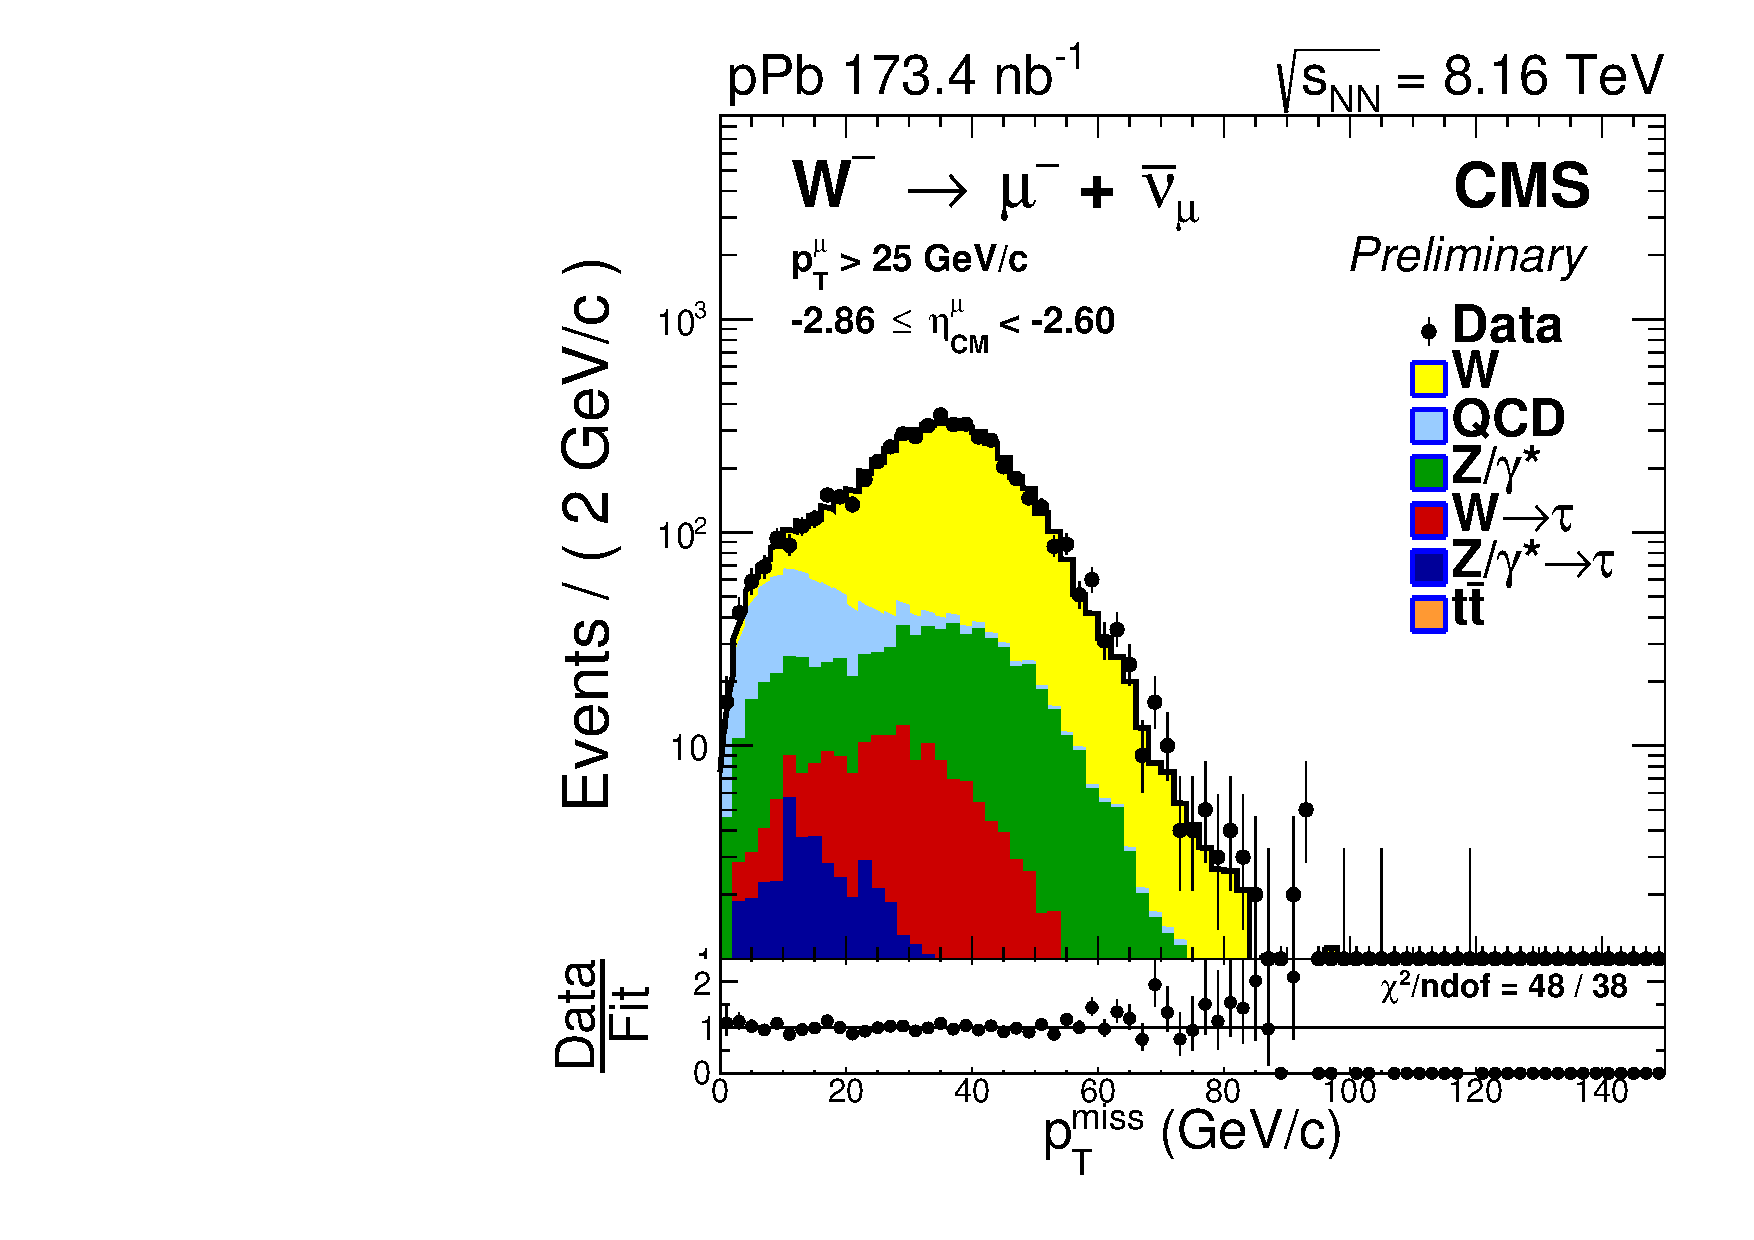
\includegraphics[width=0.23\textwidth]{Figures/WBoson/Analysis/SignalExtraction/Signal/LOG/PLOT_MET_DATA_WToMuMi_PA_Model_TEMP_WDYDYToTauWToTauTTbar_ModifiedRayleigh_QCD_MuEtaCM_-286_-260_MuIso_0_15.pdf}
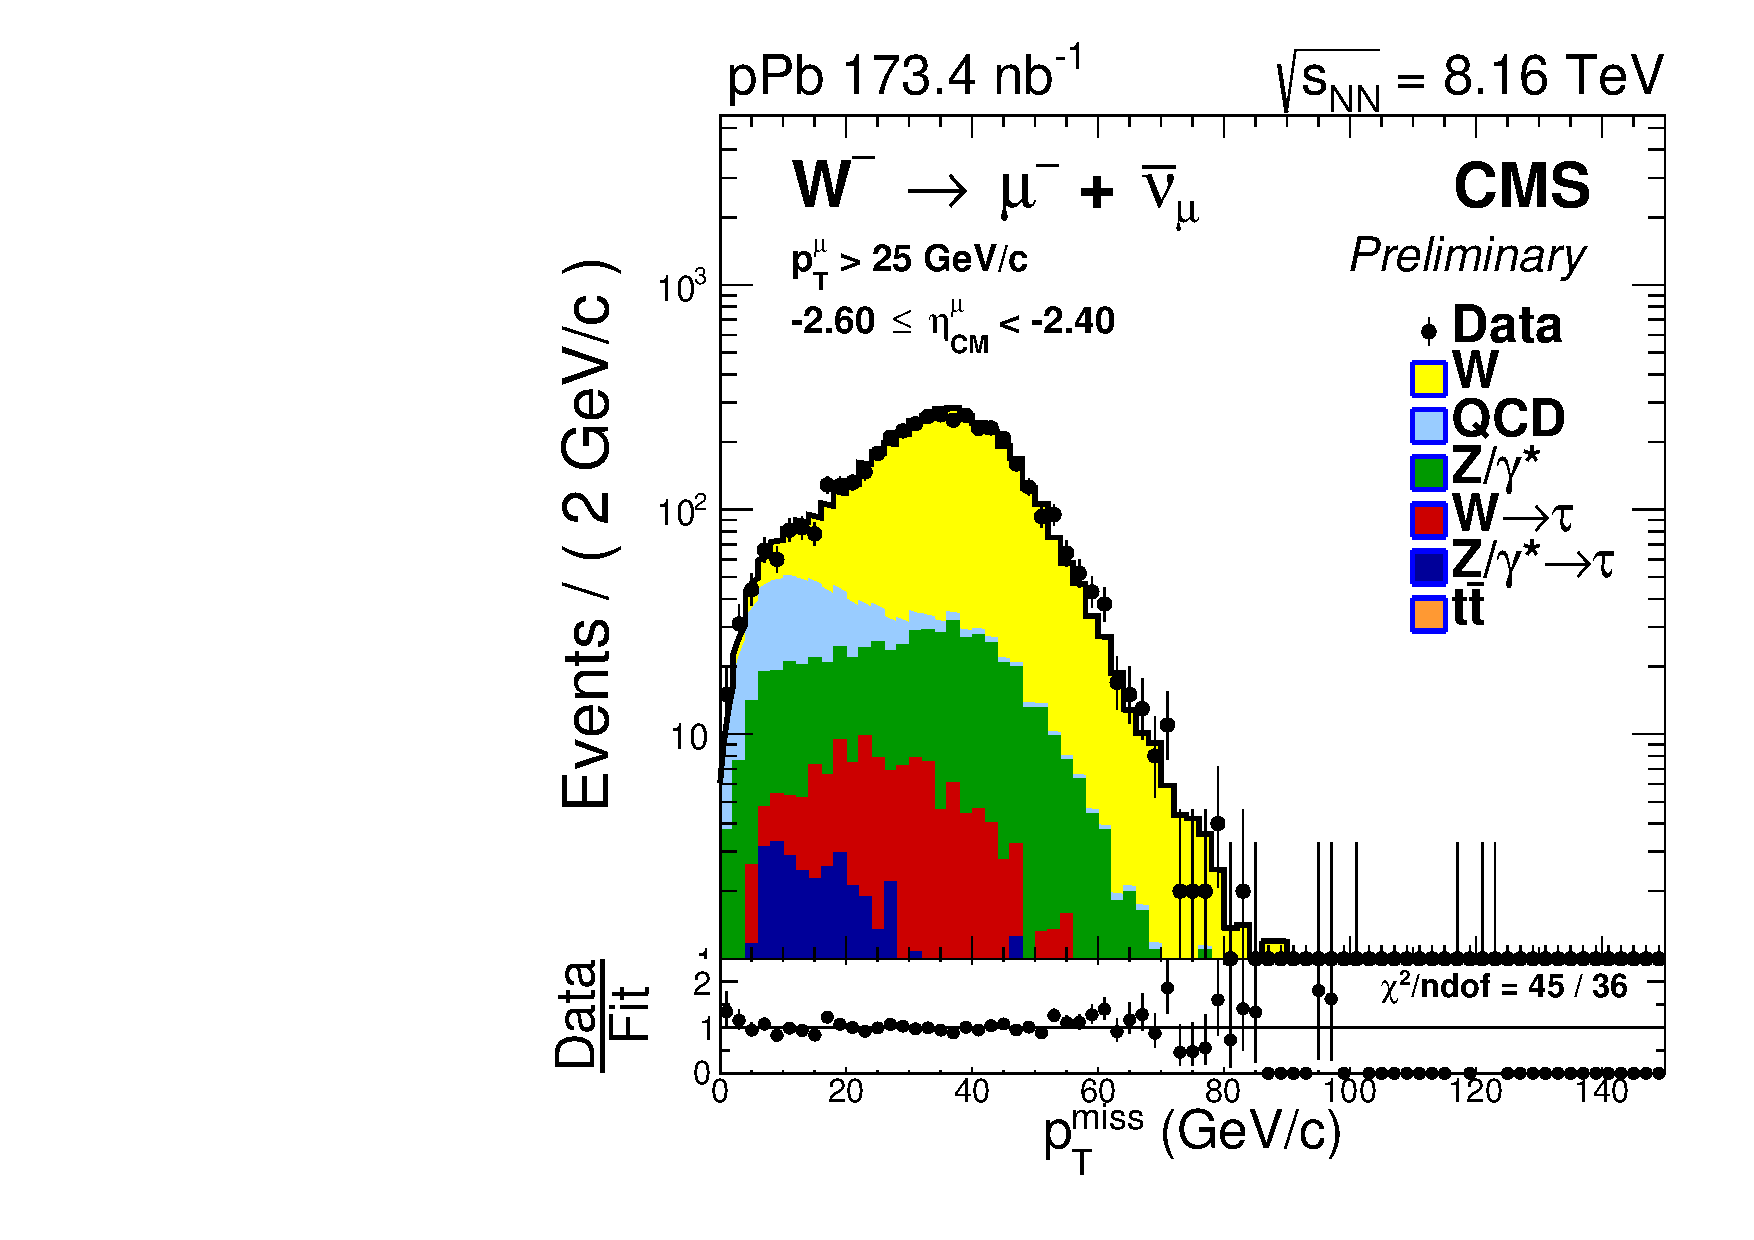
\includegraphics[width=0.23\textwidth]{Figures/WBoson/Analysis/SignalExtraction/Signal/LOG/PLOT_MET_DATA_WToMuMi_PA_Model_TEMP_WDYDYToTauWToTauTTbar_ModifiedRayleigh_QCD_MuEtaCM_-260_-240_MuIso_0_15.pdf}
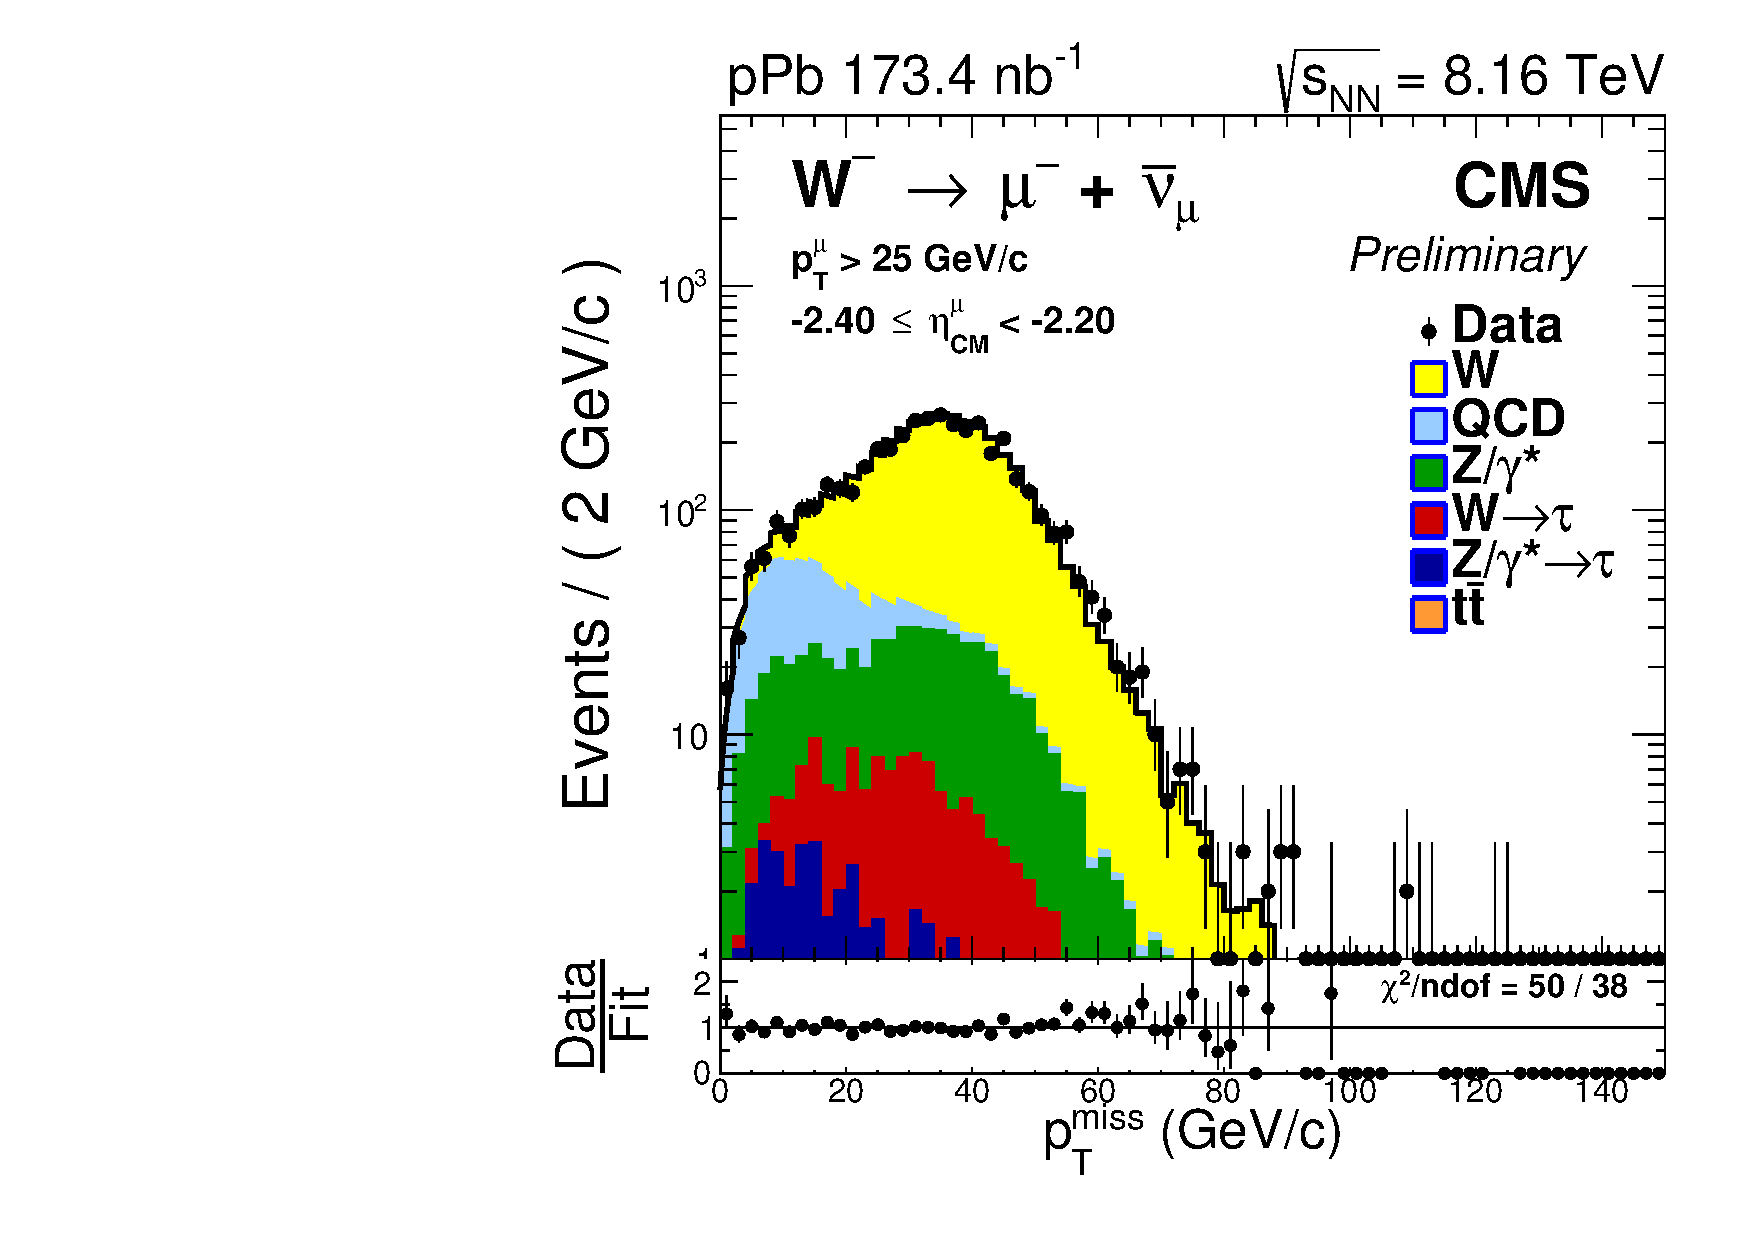
\includegraphics[width=0.23\textwidth]{Figures/WBoson/Analysis/SignalExtraction/Signal/LOG/PLOT_MET_DATA_WToMuMi_PA_Model_TEMP_WDYDYToTauWToTauTTbar_ModifiedRayleigh_QCD_MuEtaCM_-240_-220_MuIso_0_15.pdf}
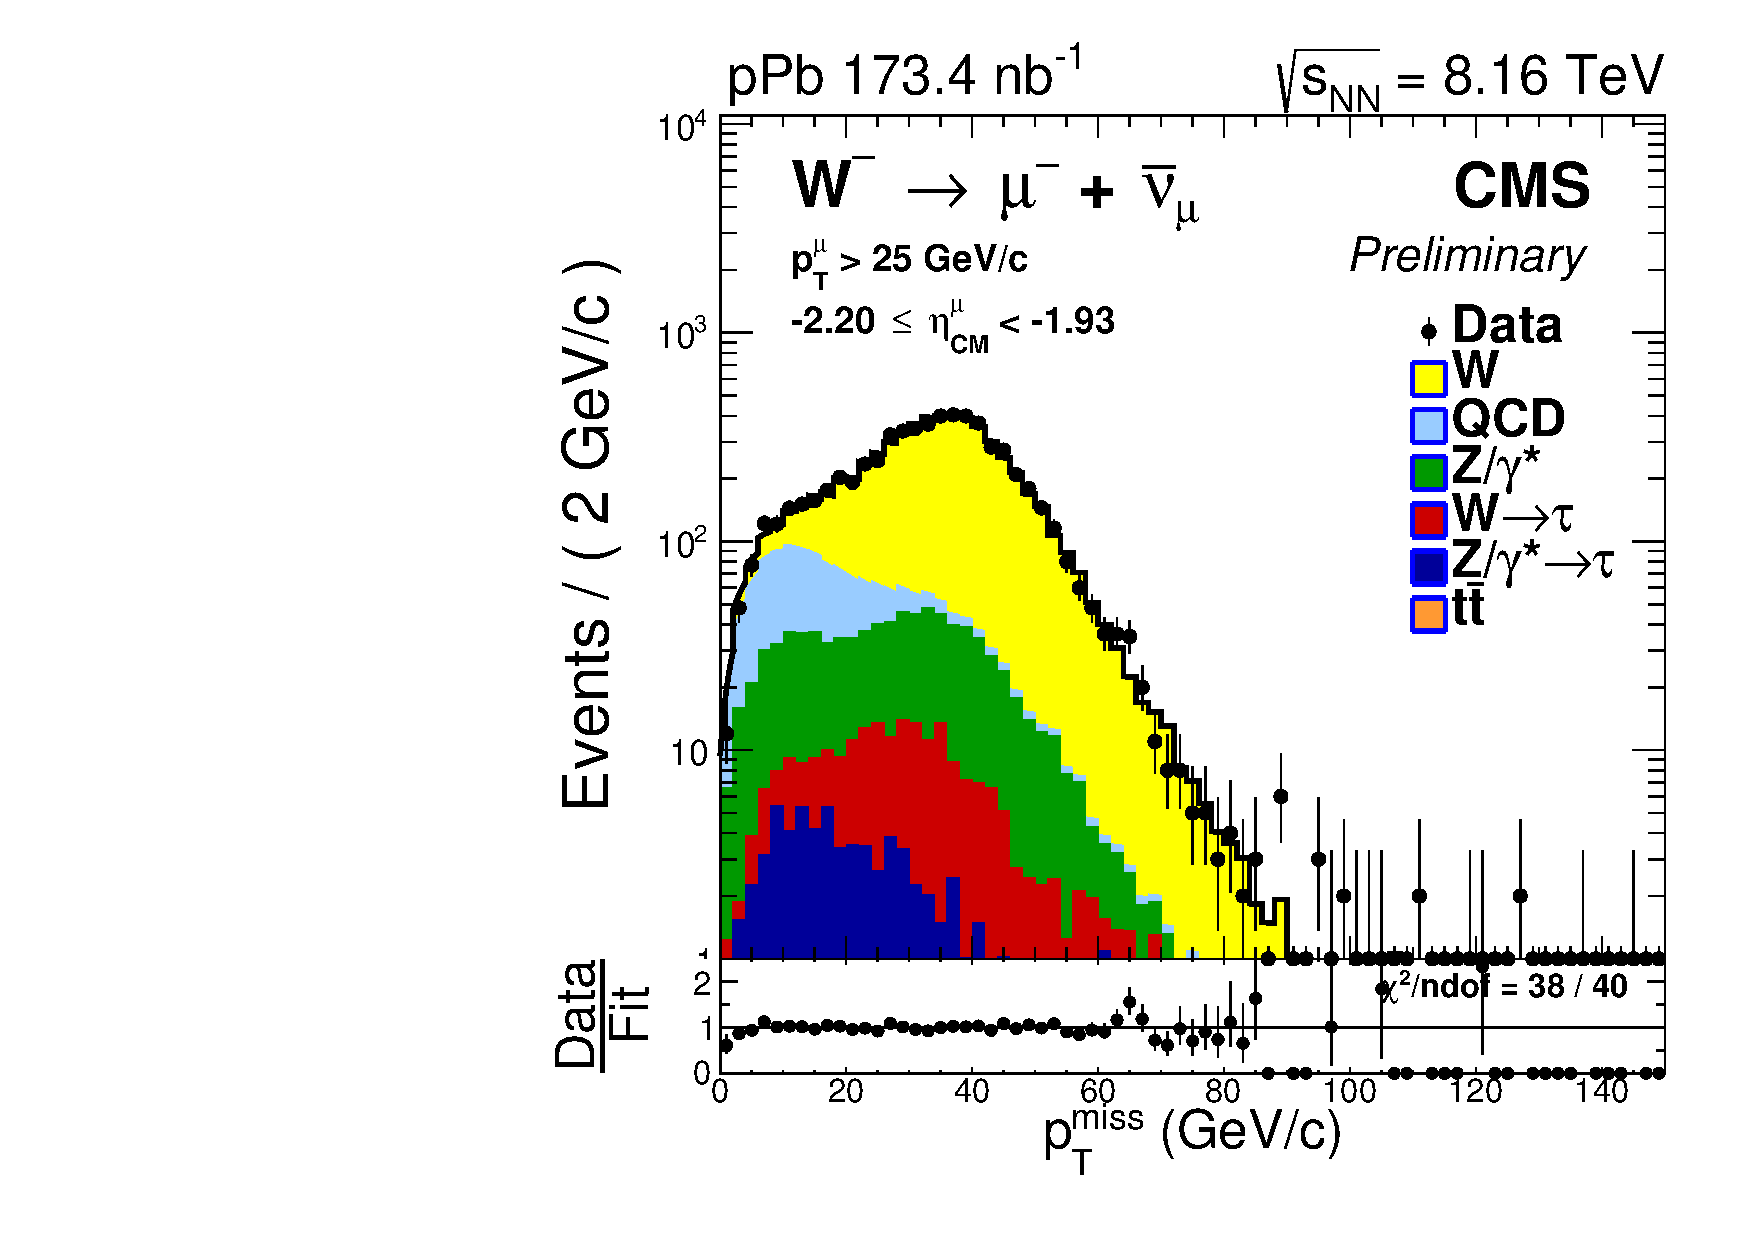
\includegraphics[width=0.23\textwidth]{Figures/WBoson/Analysis/SignalExtraction/Signal/LOG/PLOT_MET_DATA_WToMuMi_PA_Model_TEMP_WDYDYToTauWToTauTTbar_ModifiedRayleigh_QCD_MuEtaCM_-220_-193_MuIso_0_15.pdf}
\\
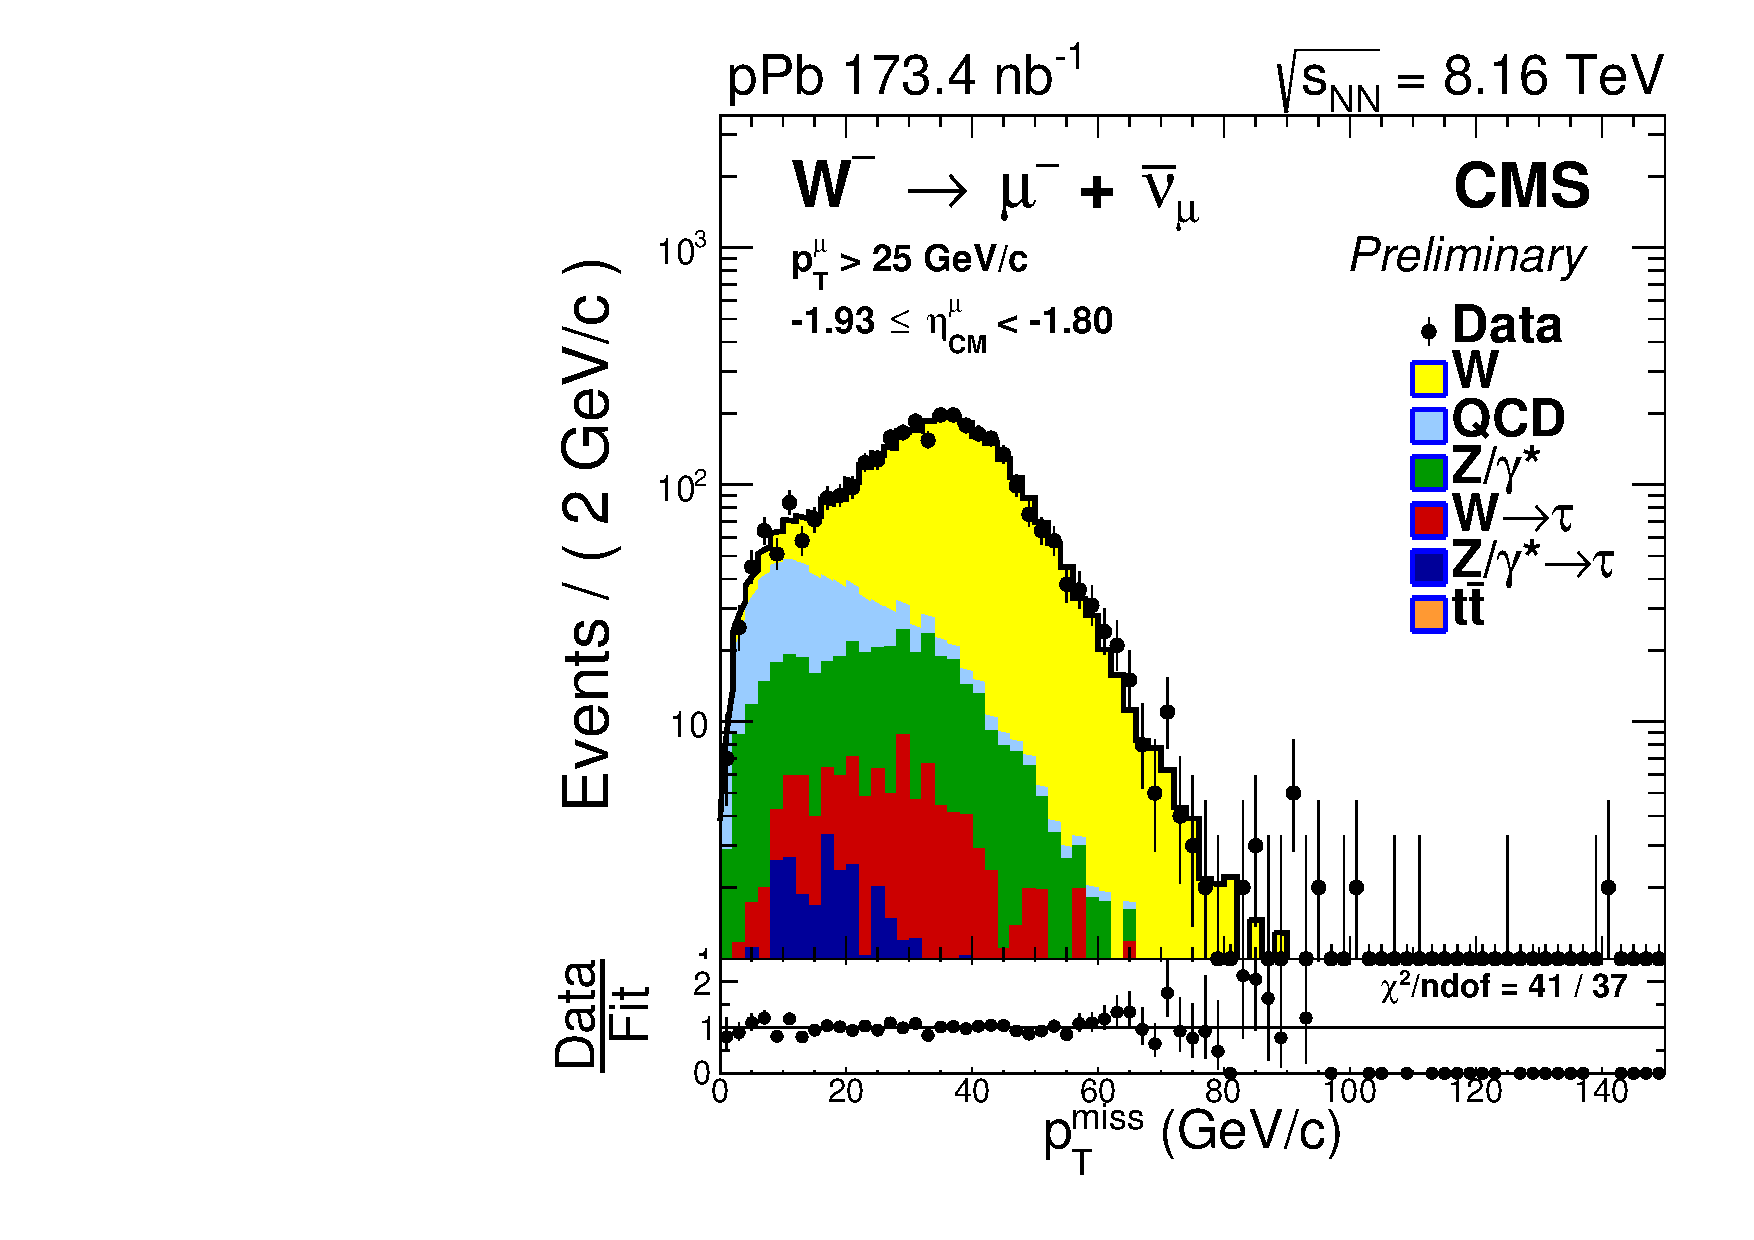
\includegraphics[width=0.23\textwidth]{Figures/WBoson/Analysis/SignalExtraction/Signal/LOG/PLOT_MET_DATA_WToMuMi_PA_Model_TEMP_WDYDYToTauWToTauTTbar_ModifiedRayleigh_QCD_MuEtaCM_-193_-180_MuIso_0_15.pdf}
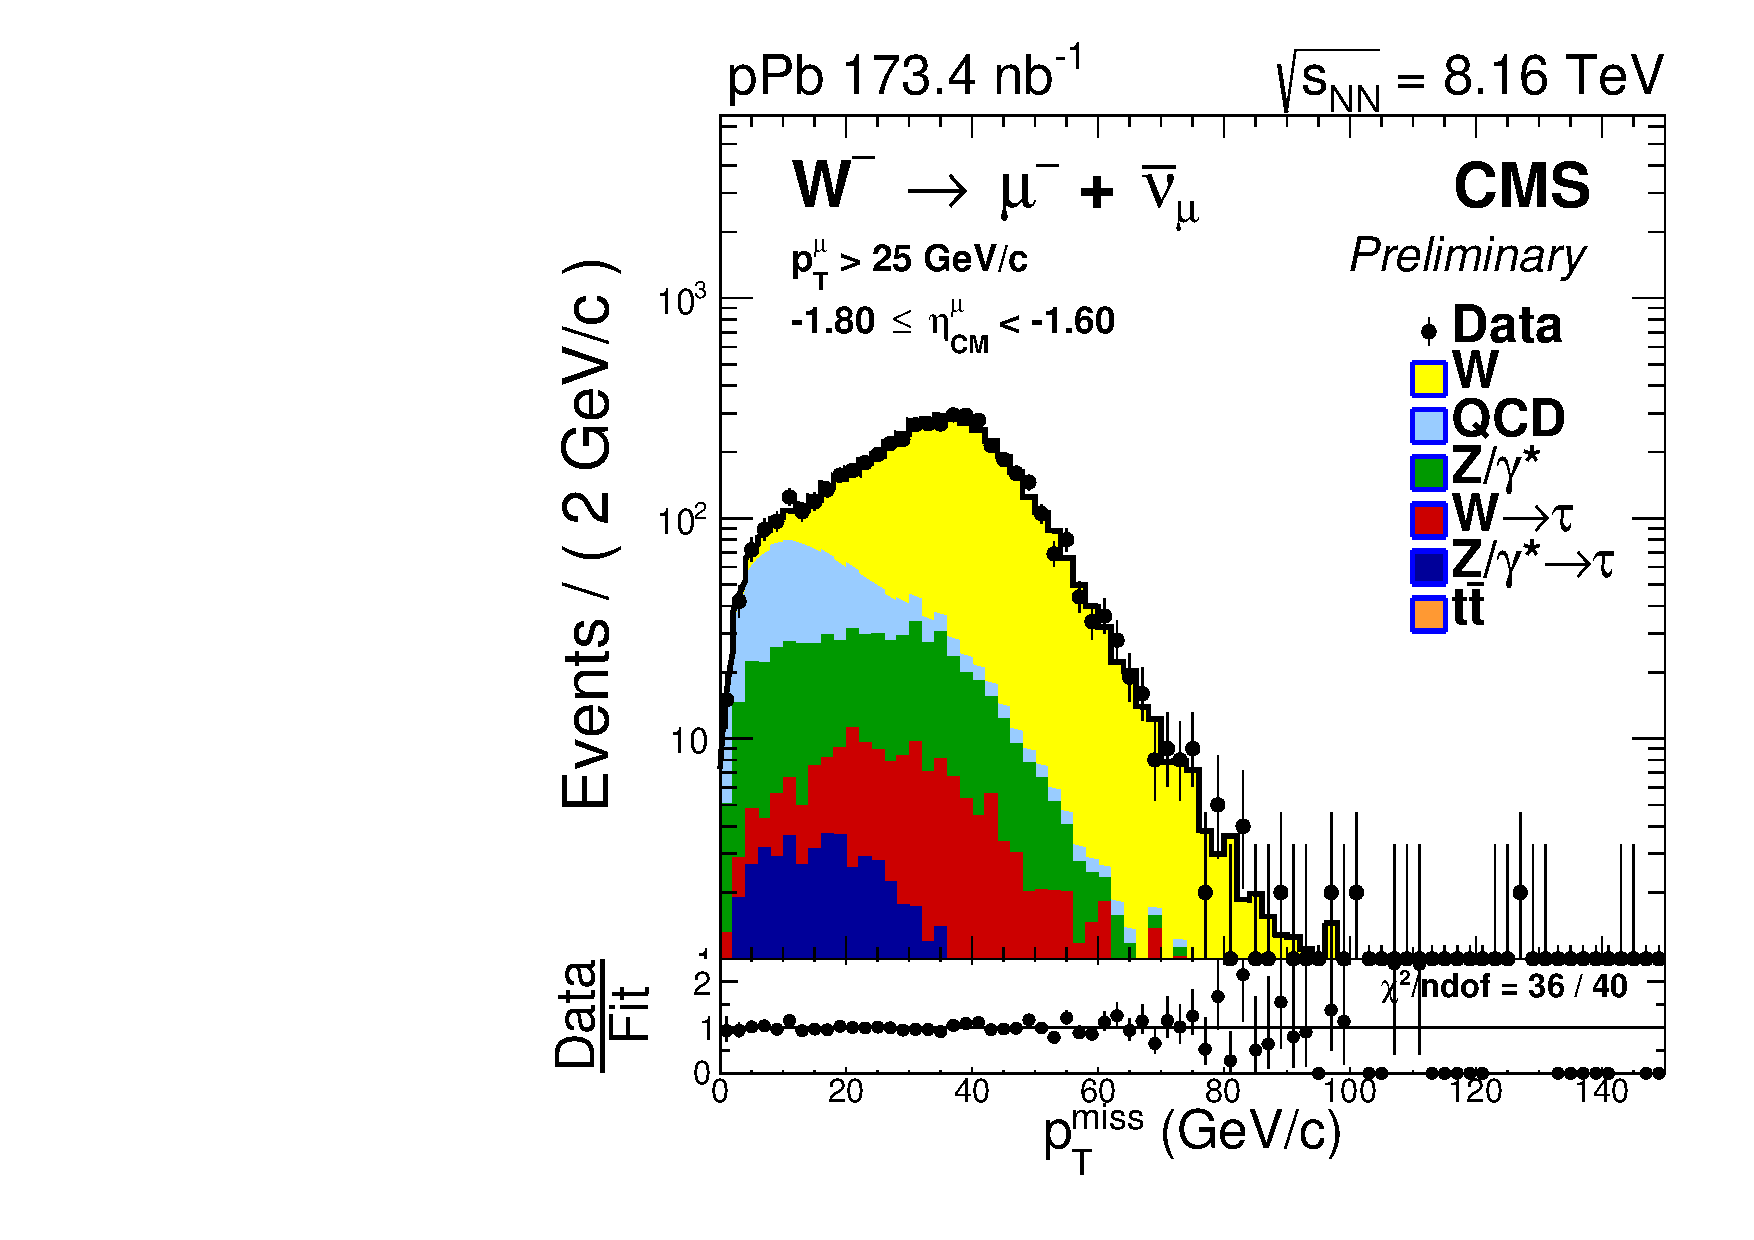
\includegraphics[width=0.23\textwidth]{Figures/WBoson/Analysis/SignalExtraction/Signal/LOG/PLOT_MET_DATA_WToMuMi_PA_Model_TEMP_WDYDYToTauWToTauTTbar_ModifiedRayleigh_QCD_MuEtaCM_-180_-160_MuIso_0_15.pdf}
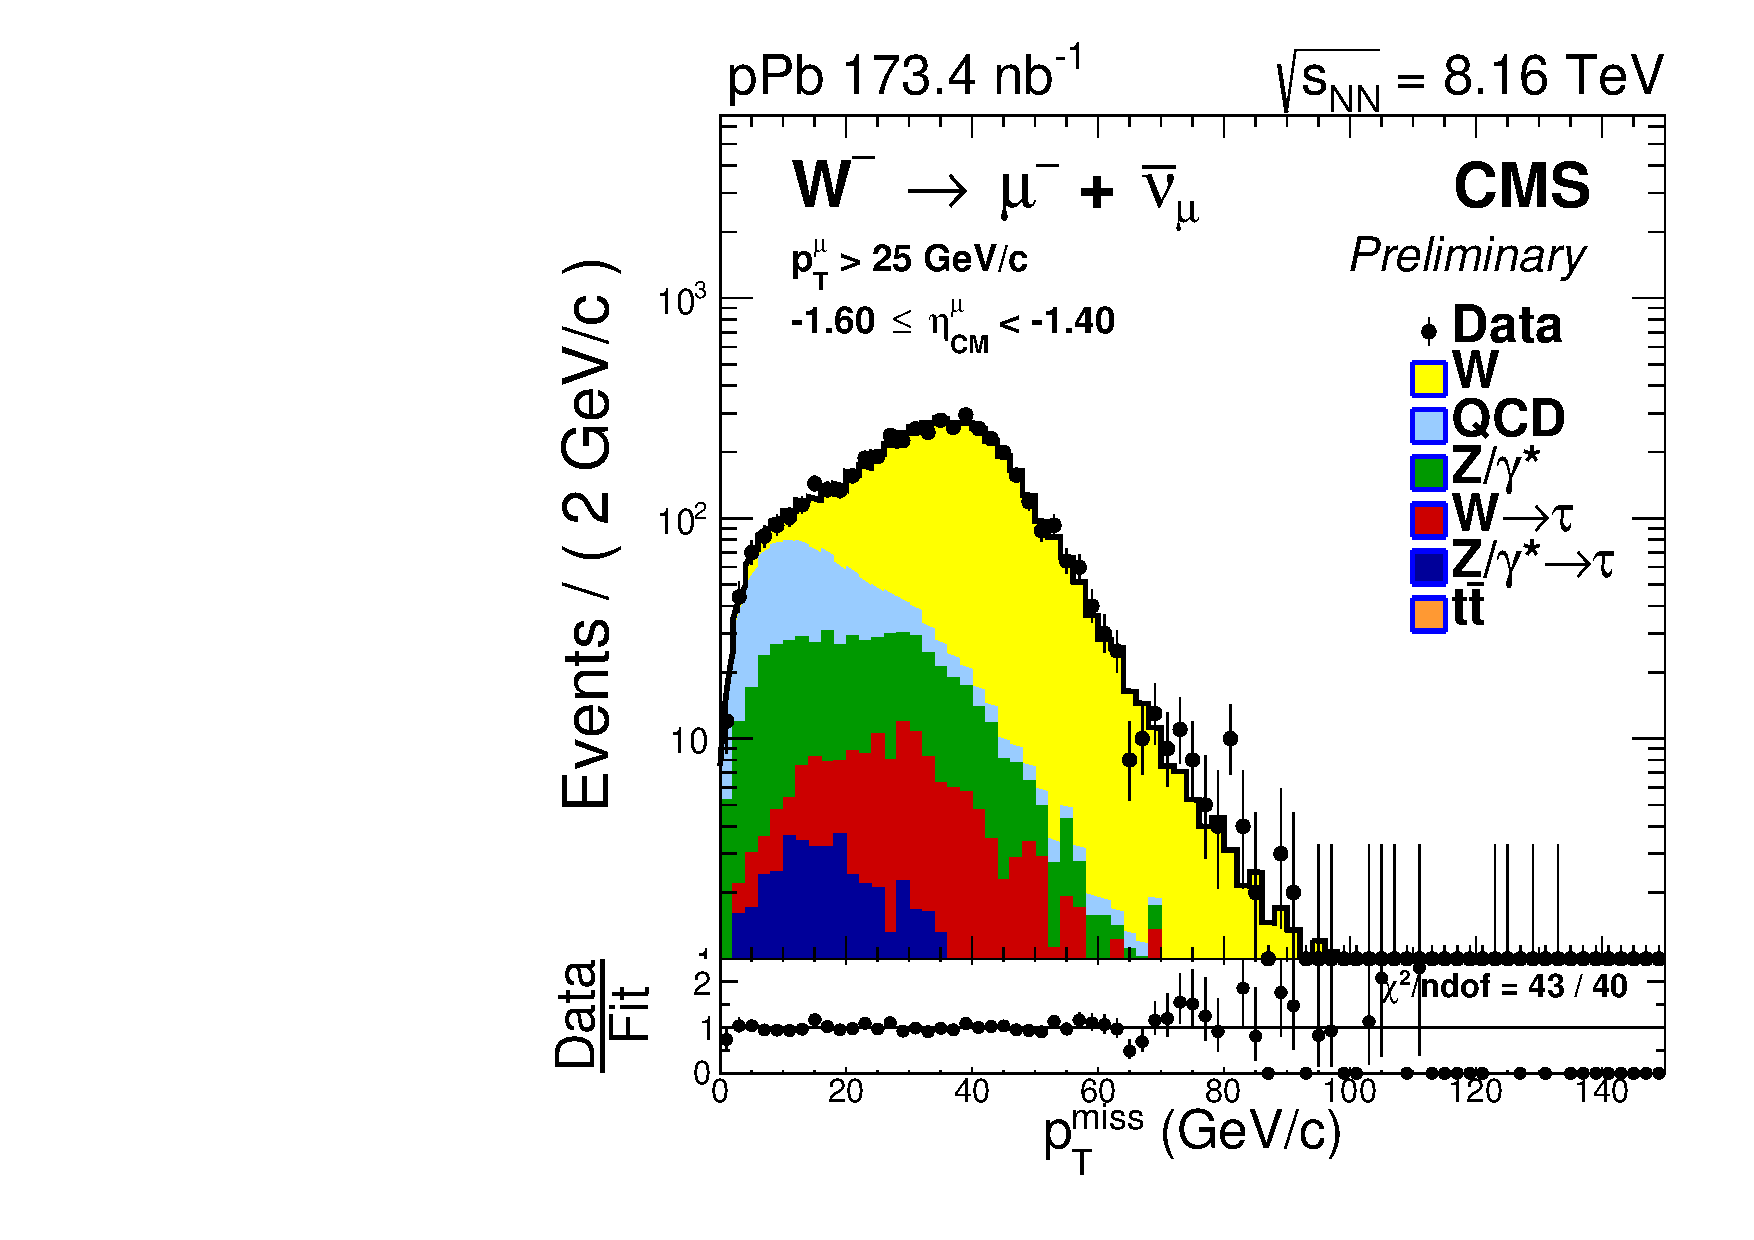
\includegraphics[width=0.23\textwidth]{Figures/WBoson/Analysis/SignalExtraction/Signal/LOG/PLOT_MET_DATA_WToMuMi_PA_Model_TEMP_WDYDYToTauWToTauTTbar_ModifiedRayleigh_QCD_MuEtaCM_-160_-140_MuIso_0_15.pdf}
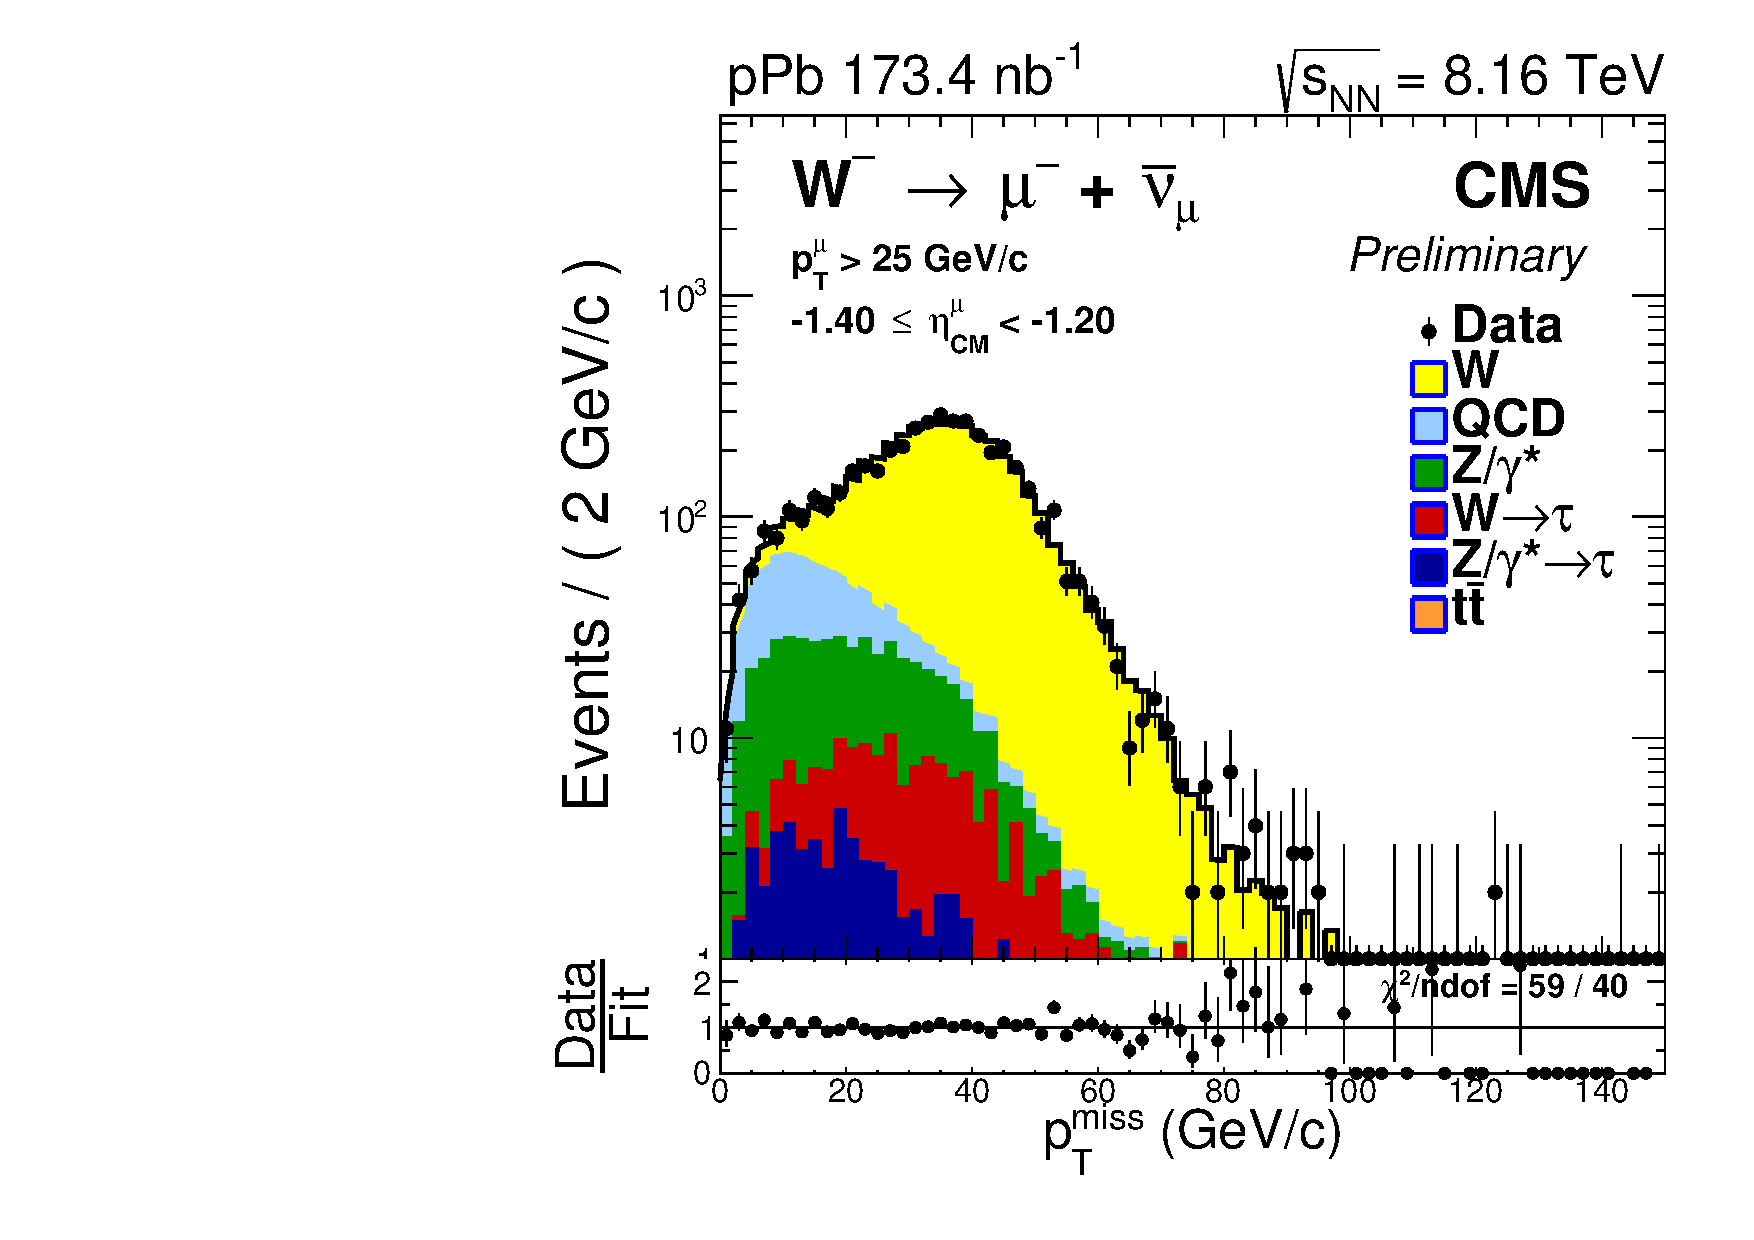
\includegraphics[width=0.23\textwidth]{Figures/WBoson/Analysis/SignalExtraction/Signal/LOG/PLOT_MET_DATA_WToMuMi_PA_Model_TEMP_WDYDYToTauWToTauTTbar_ModifiedRayleigh_QCD_MuEtaCM_-140_-120_MuIso_0_15.pdf}
\\
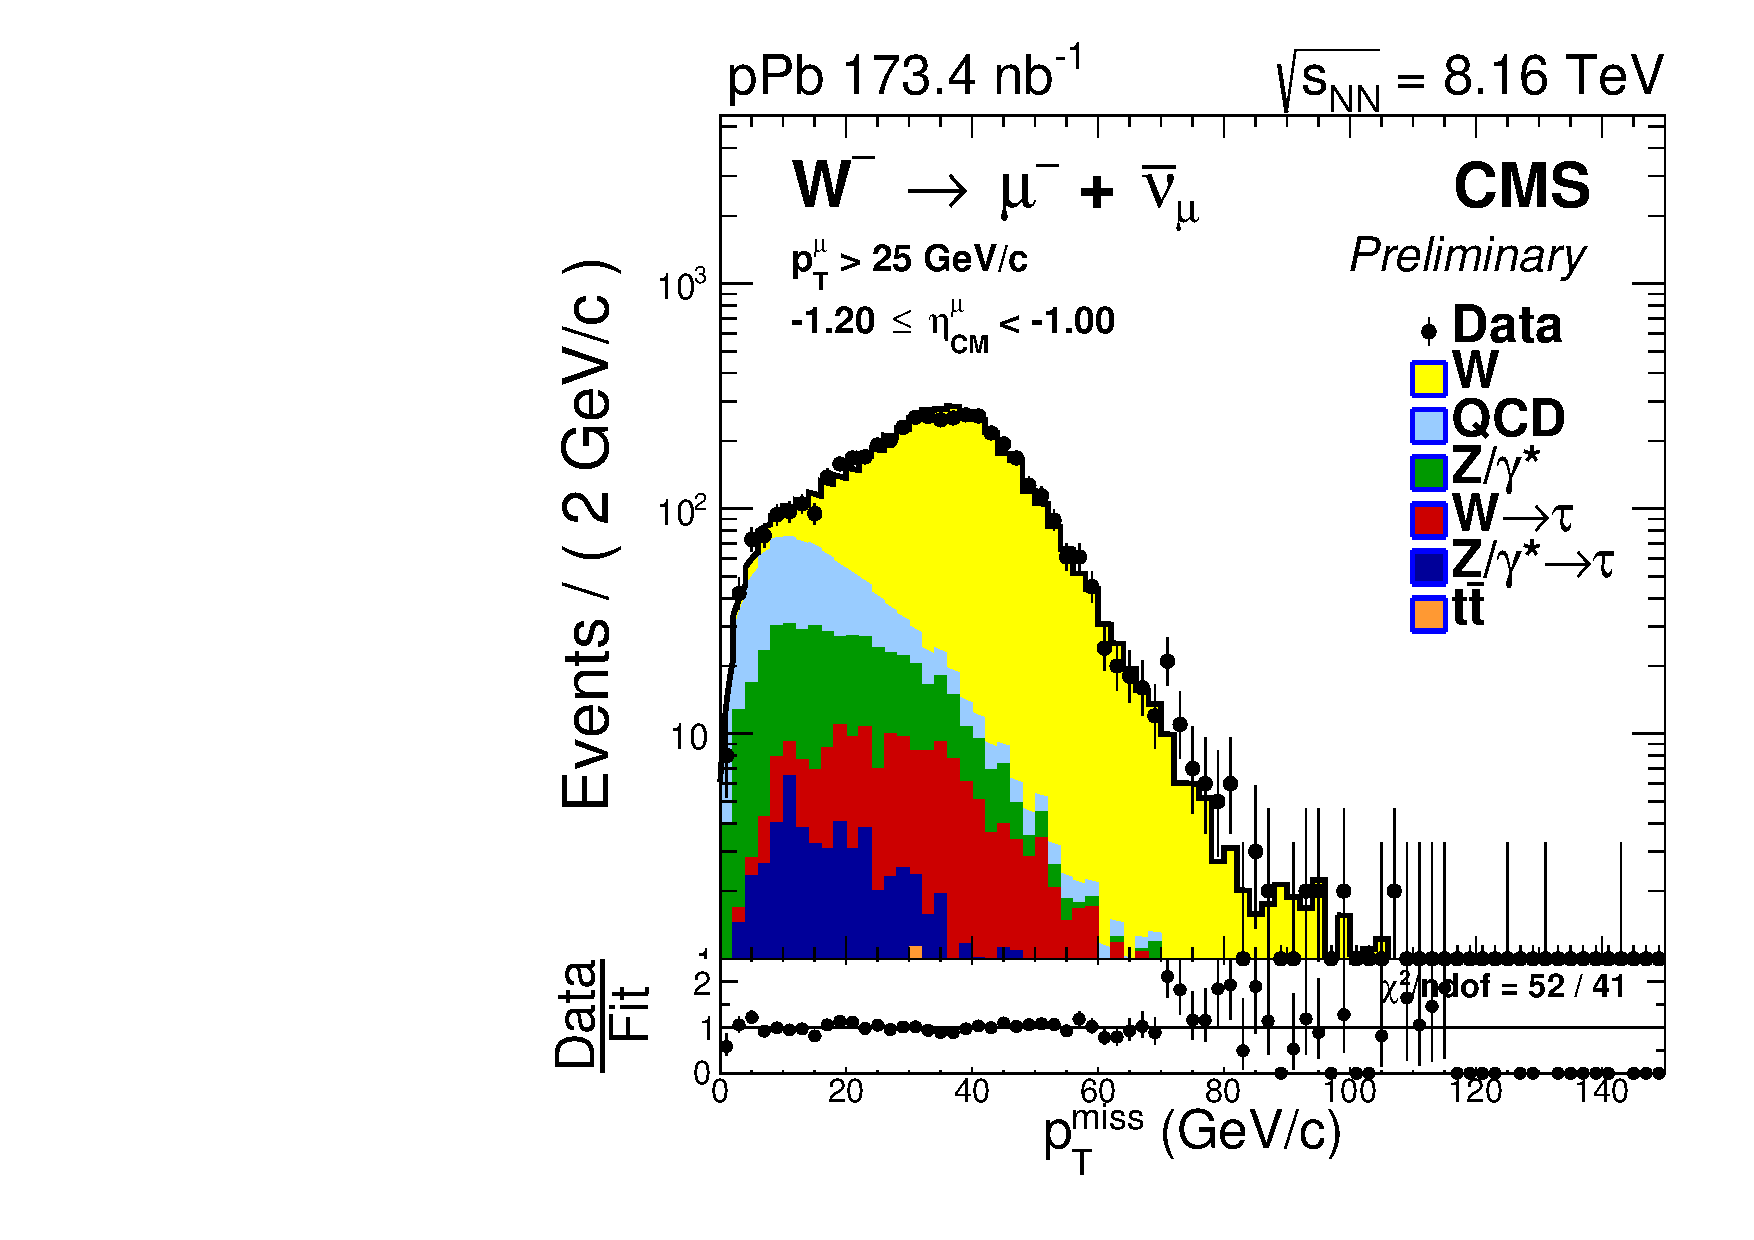
\includegraphics[width=0.23\textwidth]{Figures/WBoson/Analysis/SignalExtraction/Signal/LOG/PLOT_MET_DATA_WToMuMi_PA_Model_TEMP_WDYDYToTauWToTauTTbar_ModifiedRayleigh_QCD_MuEtaCM_-120_-100_MuIso_0_15.pdf}
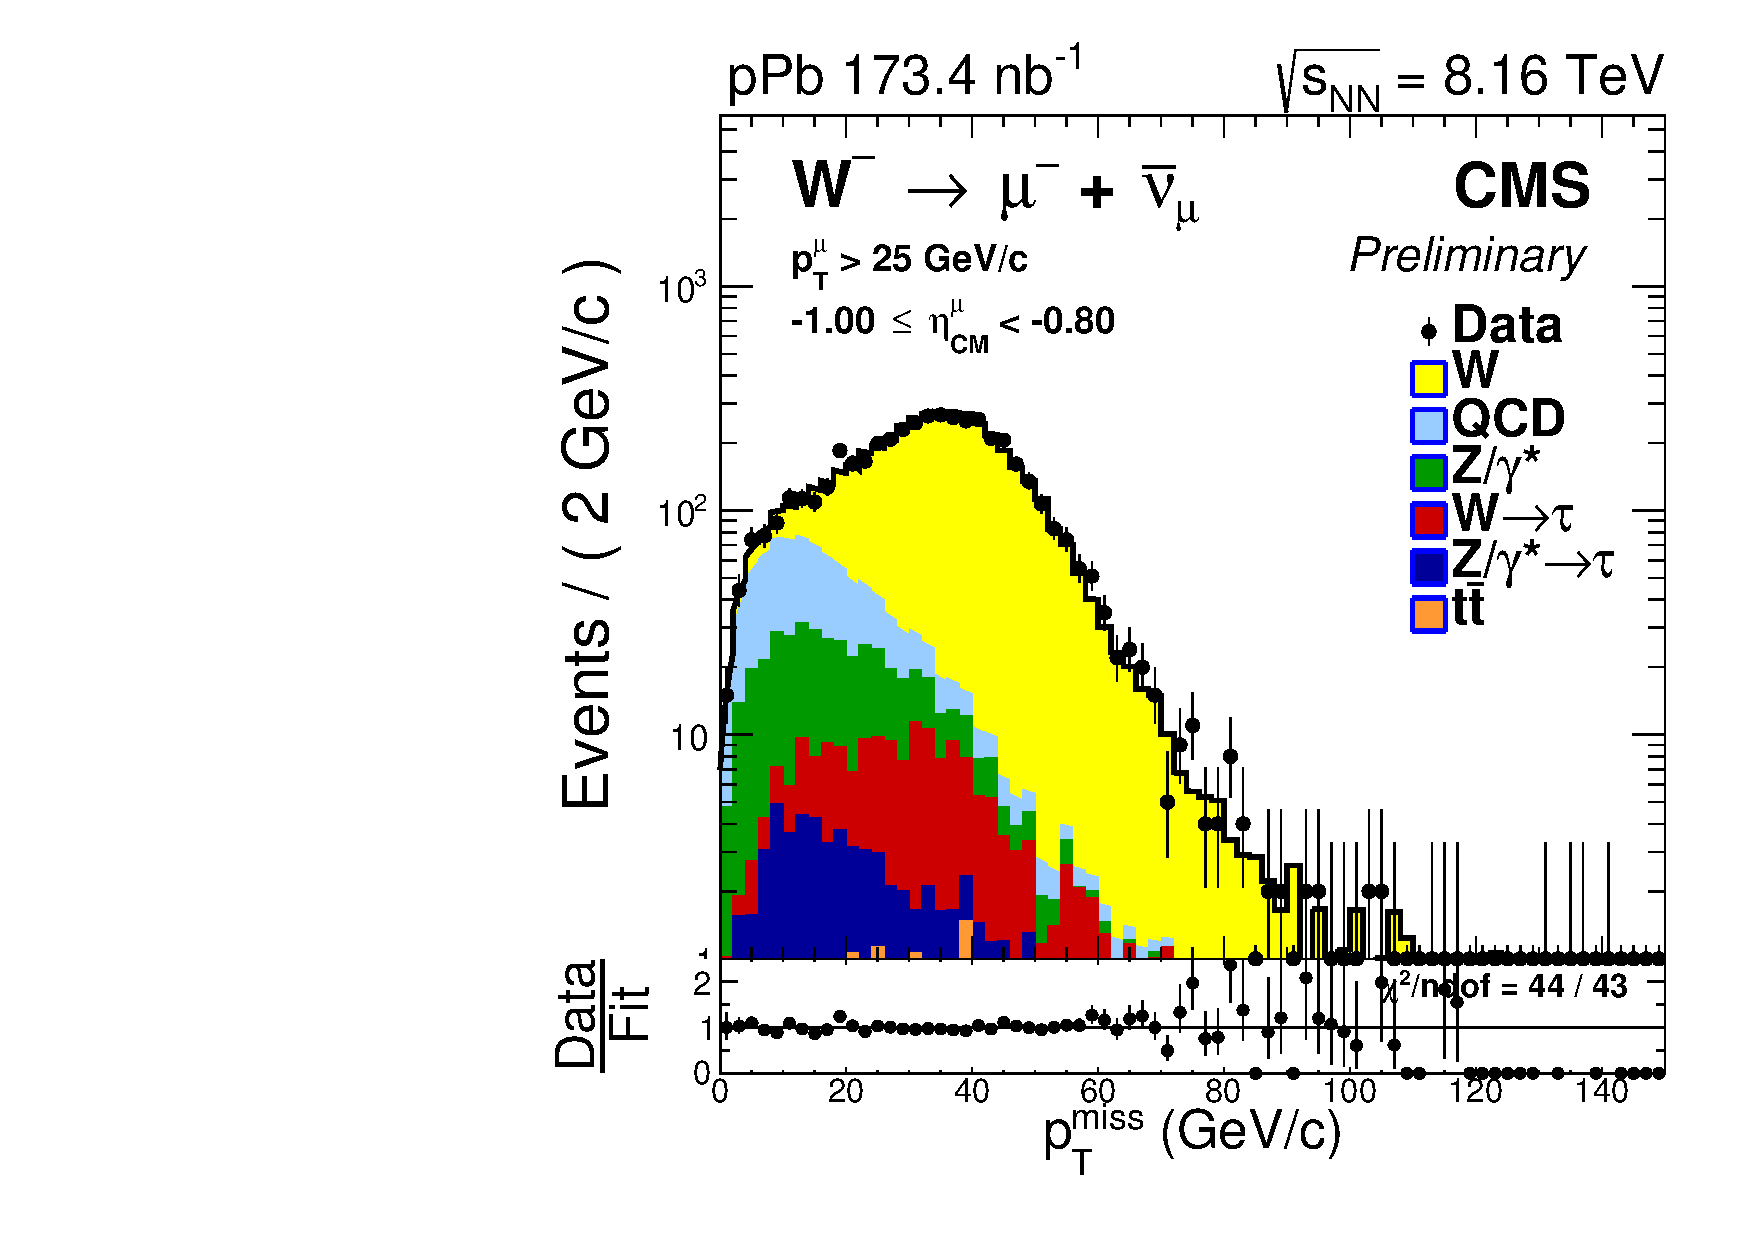
\includegraphics[width=0.23\textwidth]{Figures/WBoson/Analysis/SignalExtraction/Signal/LOG/PLOT_MET_DATA_WToMuMi_PA_Model_TEMP_WDYDYToTauWToTauTTbar_ModifiedRayleigh_QCD_MuEtaCM_-100_-80_MuIso_0_15.pdf}
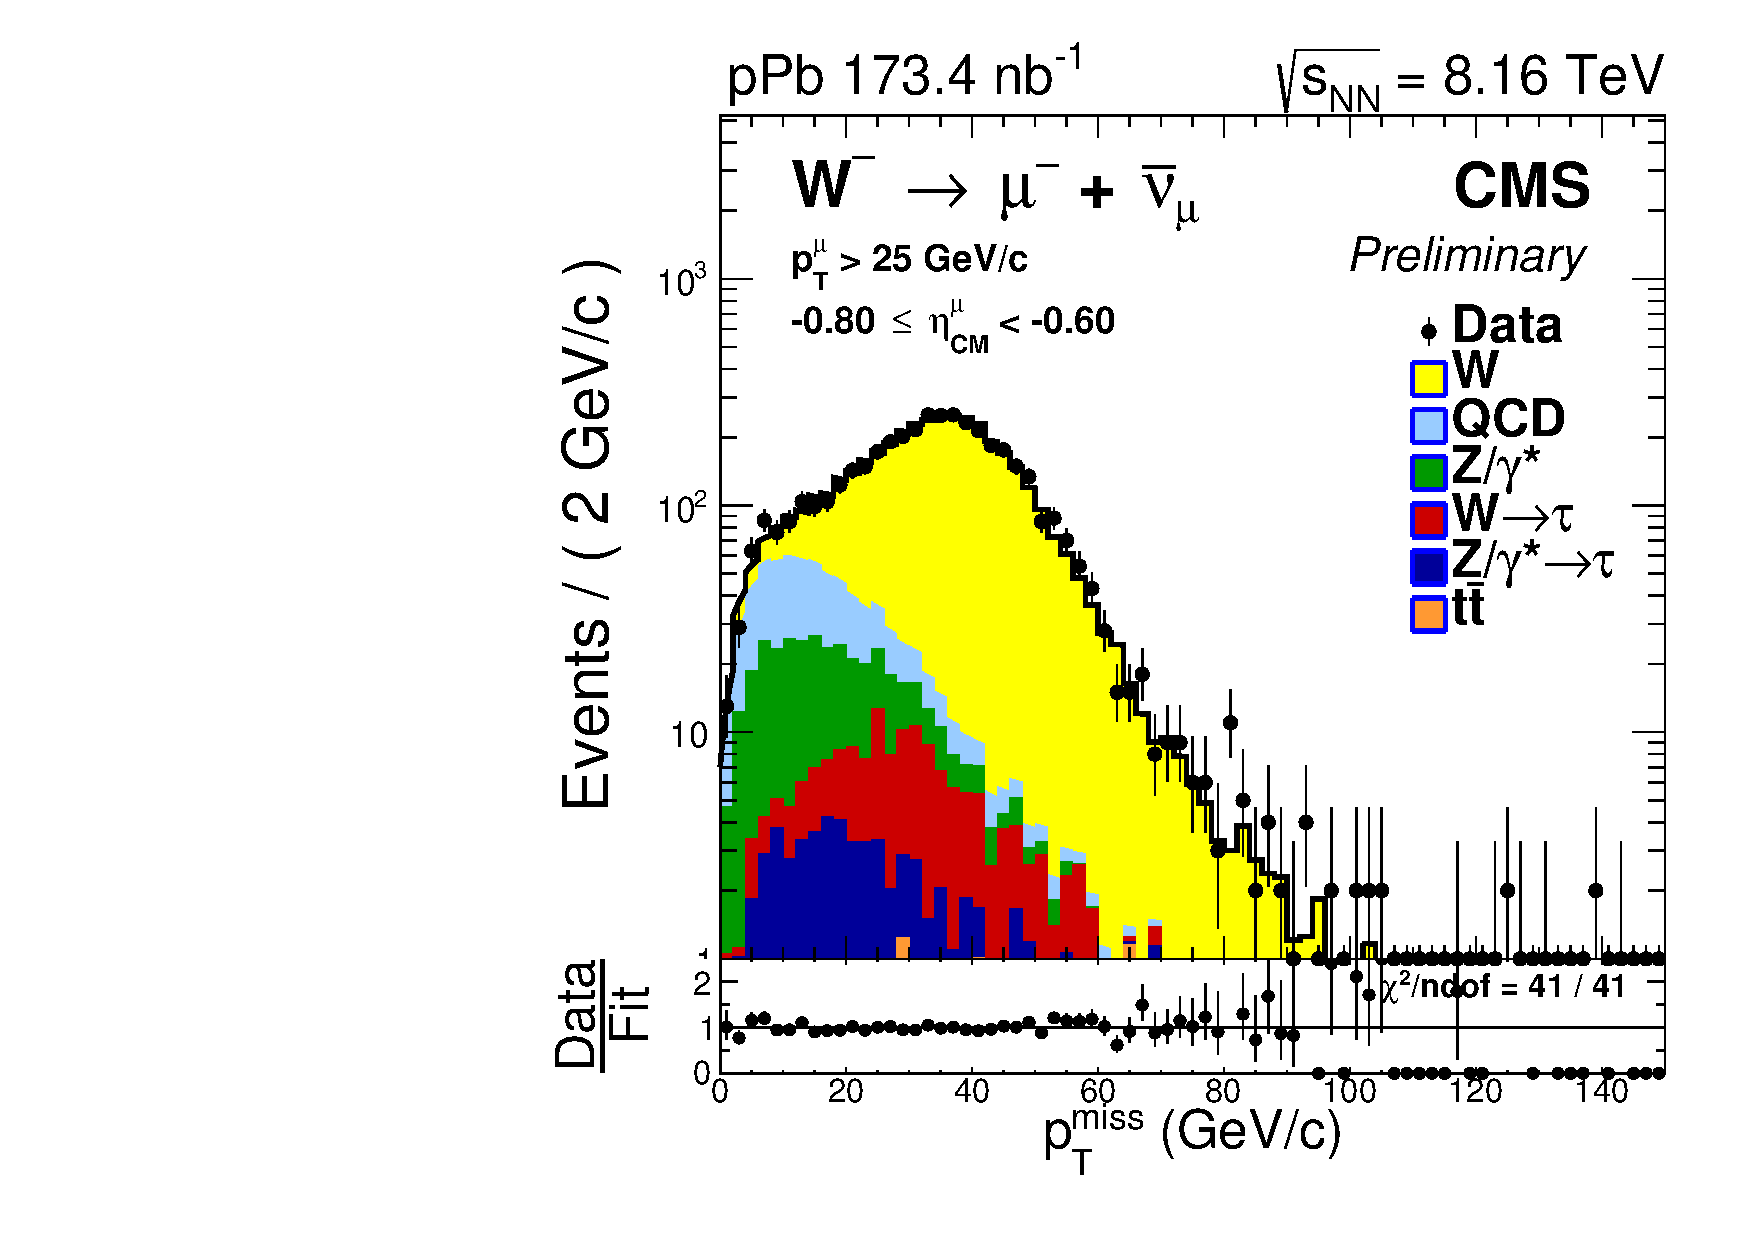
\includegraphics[width=0.23\textwidth]{Figures/WBoson/Analysis/SignalExtraction/Signal/LOG/PLOT_MET_DATA_WToMuMi_PA_Model_TEMP_WDYDYToTauWToTauTTbar_ModifiedRayleigh_QCD_MuEtaCM_-80_-60_MuIso_0_15.pdf}
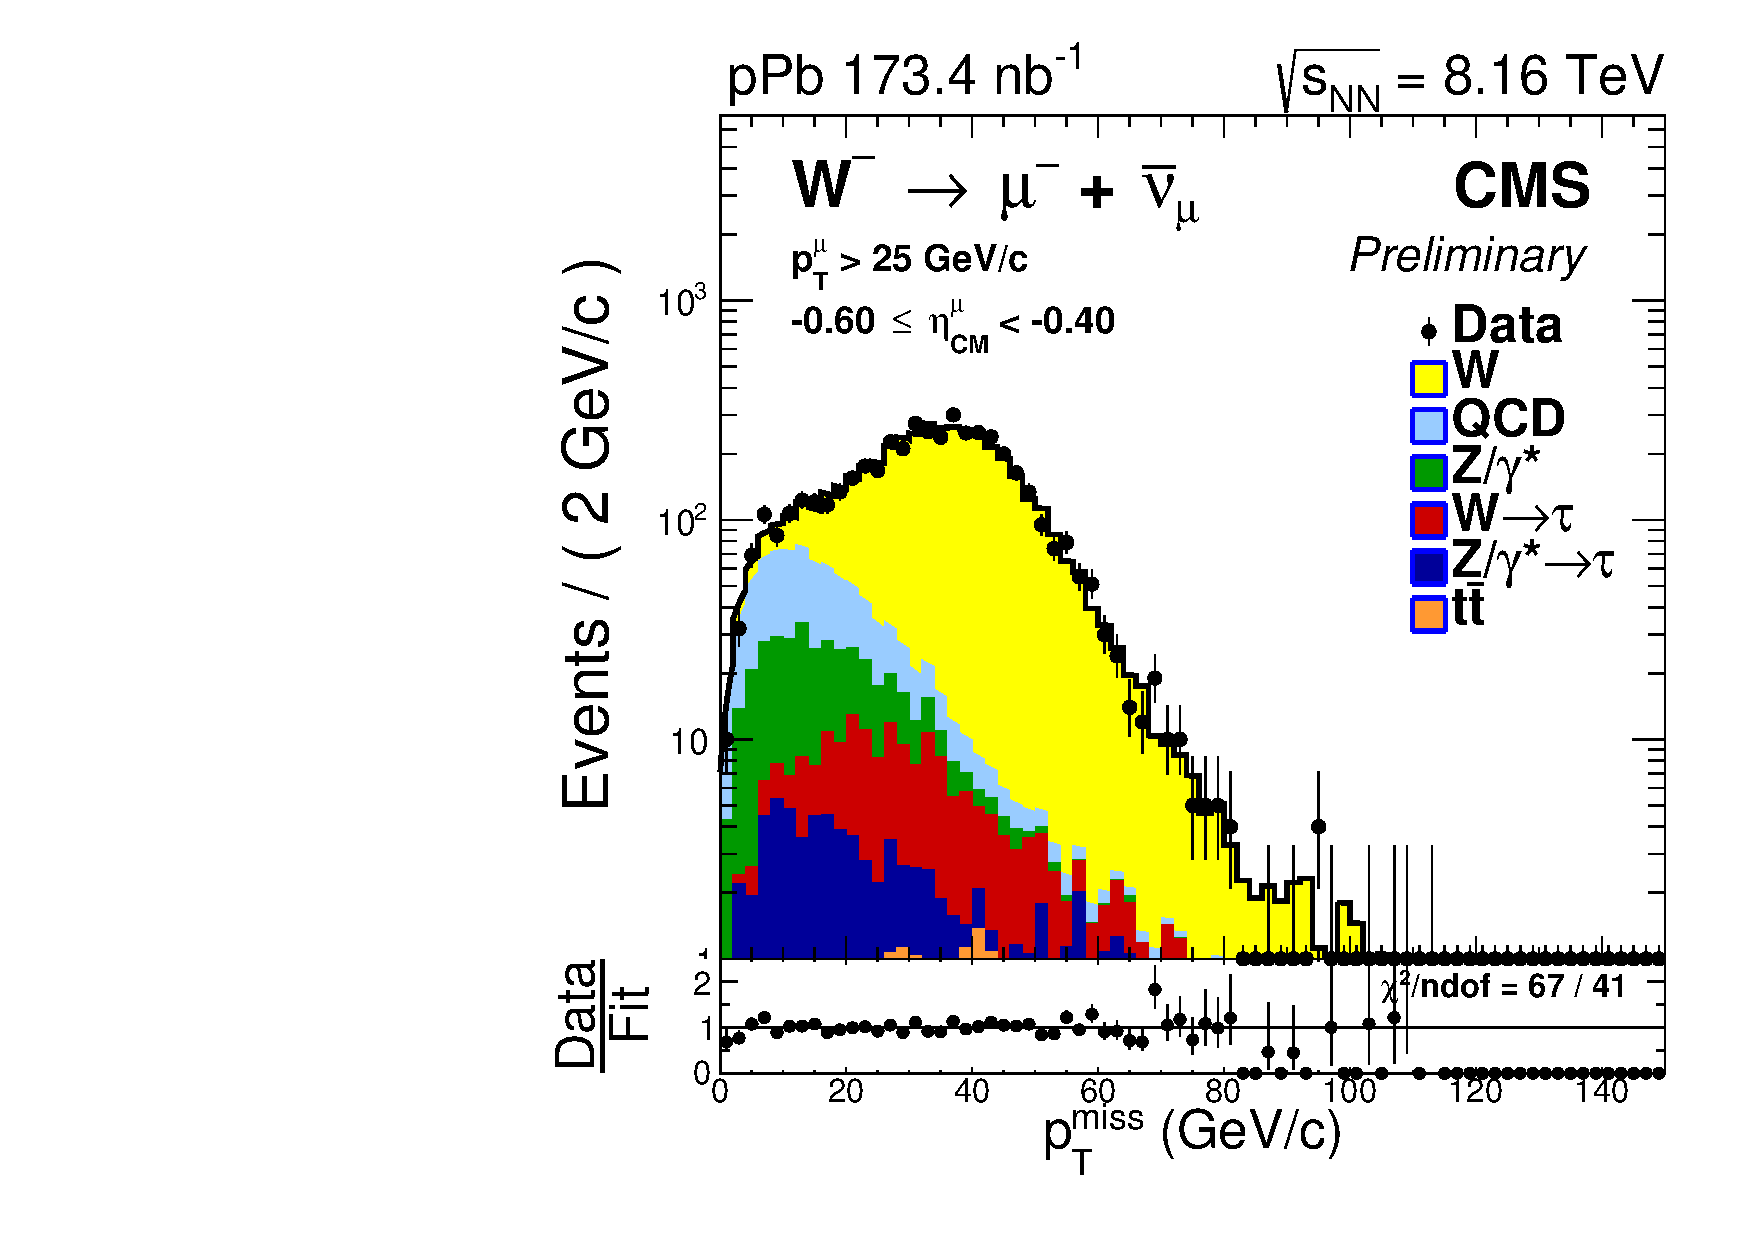
\includegraphics[width=0.23\textwidth]{Figures/WBoson/Analysis/SignalExtraction/Signal/LOG/PLOT_MET_DATA_WToMuMi_PA_Model_TEMP_WDYDYToTauWToTauTTbar_ModifiedRayleigh_QCD_MuEtaCM_-60_-40_MuIso_0_15.pdf}
\\
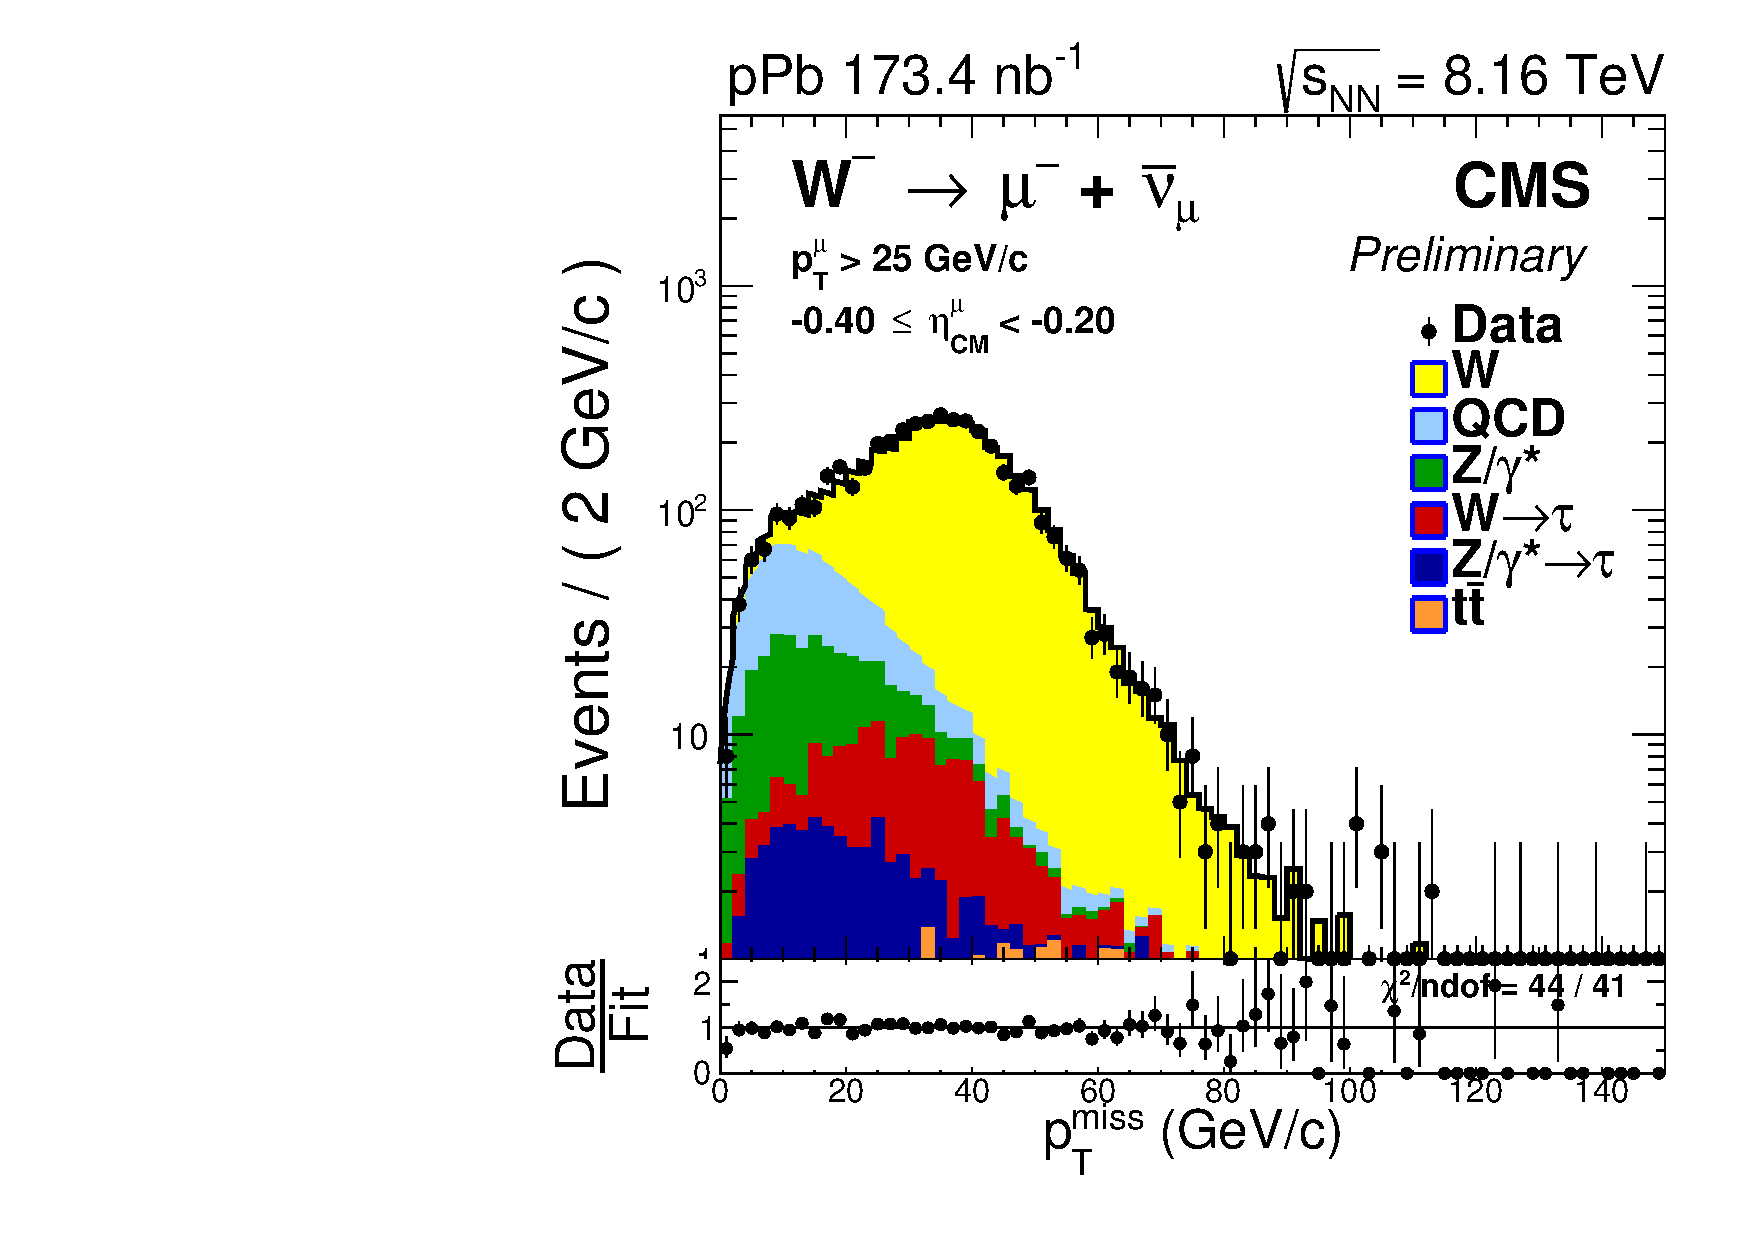
\includegraphics[width=0.23\textwidth]{Figures/WBoson/Analysis/SignalExtraction/Signal/LOG/PLOT_MET_DATA_WToMuMi_PA_Model_TEMP_WDYDYToTauWToTauTTbar_ModifiedRayleigh_QCD_MuEtaCM_-40_-20_MuIso_0_15.pdf}
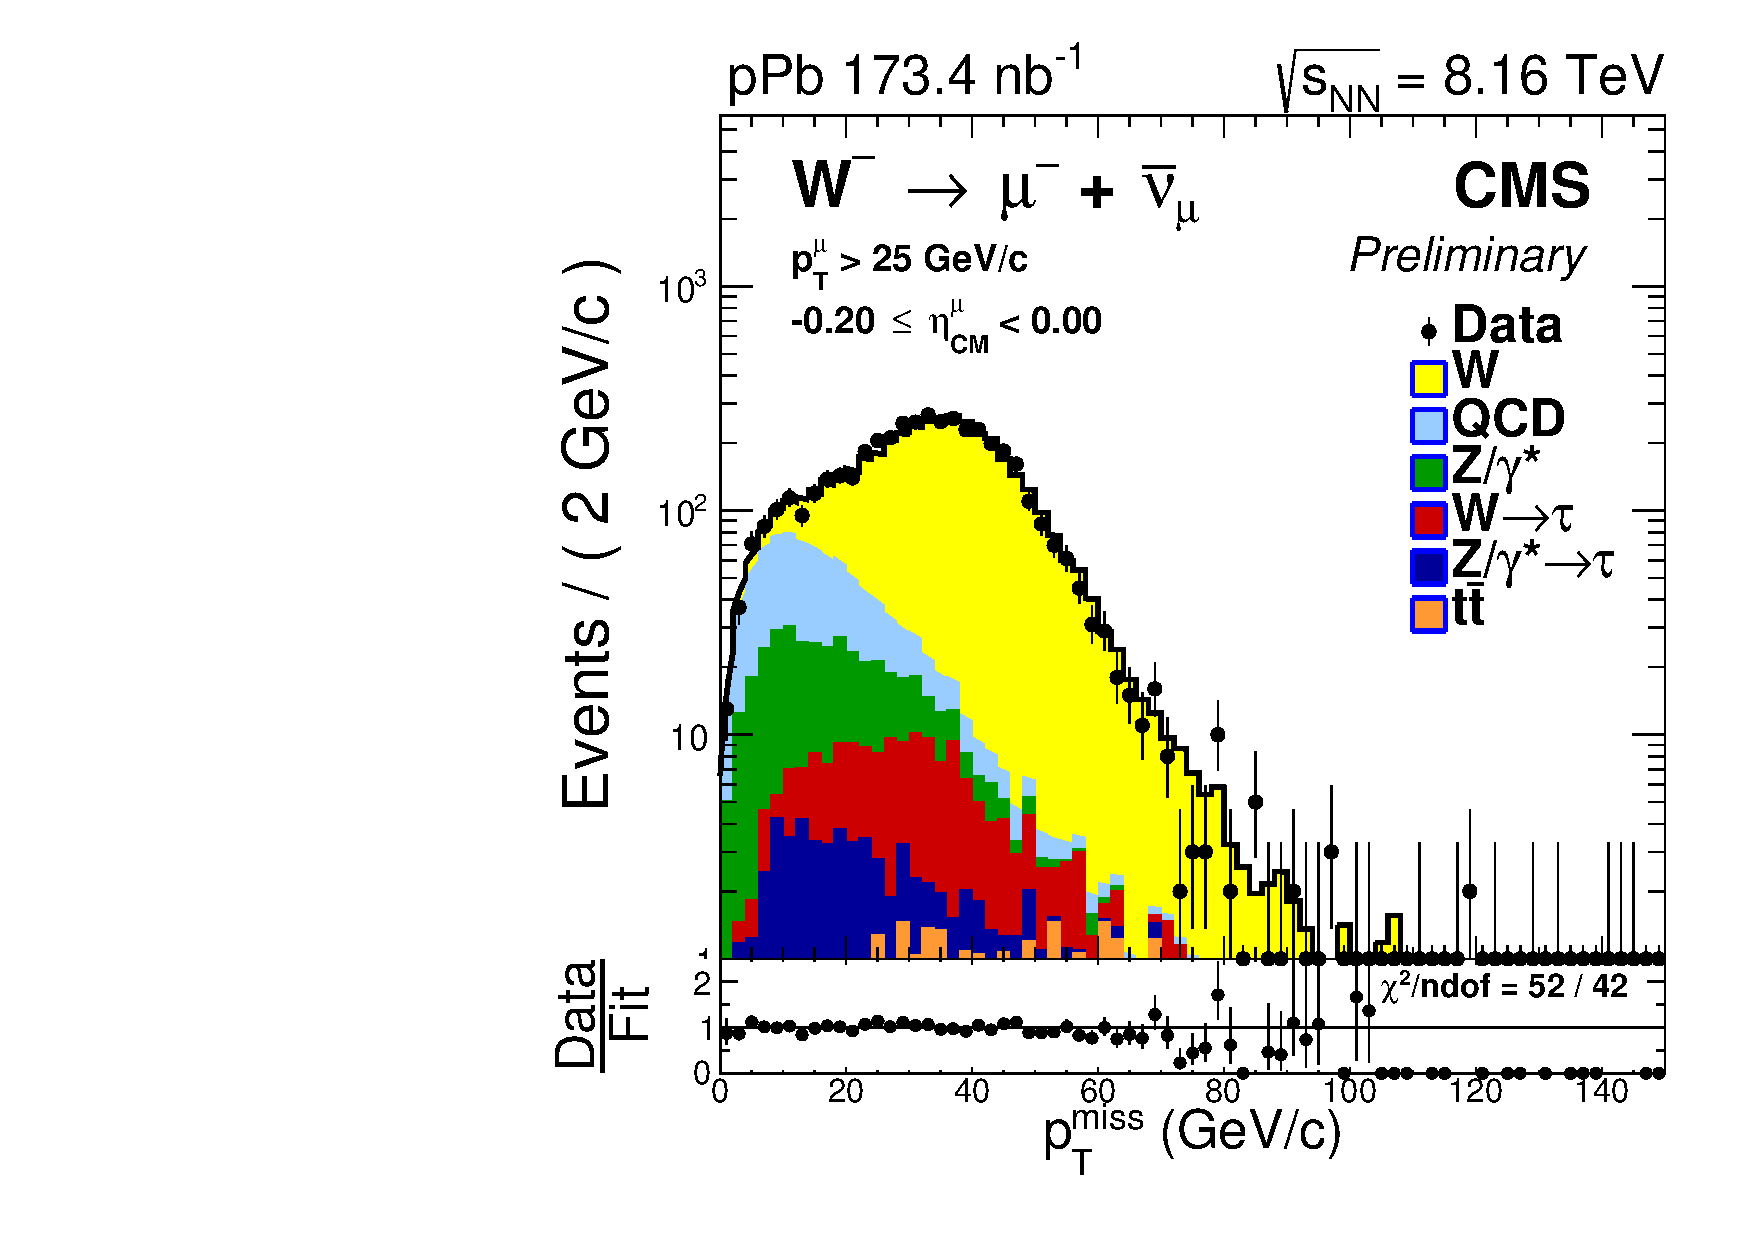
\includegraphics[width=0.23\textwidth]{Figures/WBoson/Analysis/SignalExtraction/Signal/LOG/PLOT_MET_DATA_WToMuMi_PA_Model_TEMP_WDYDYToTauWToTauTTbar_ModifiedRayleigh_QCD_MuEtaCM_-20_0_MuIso_0_15.pdf}
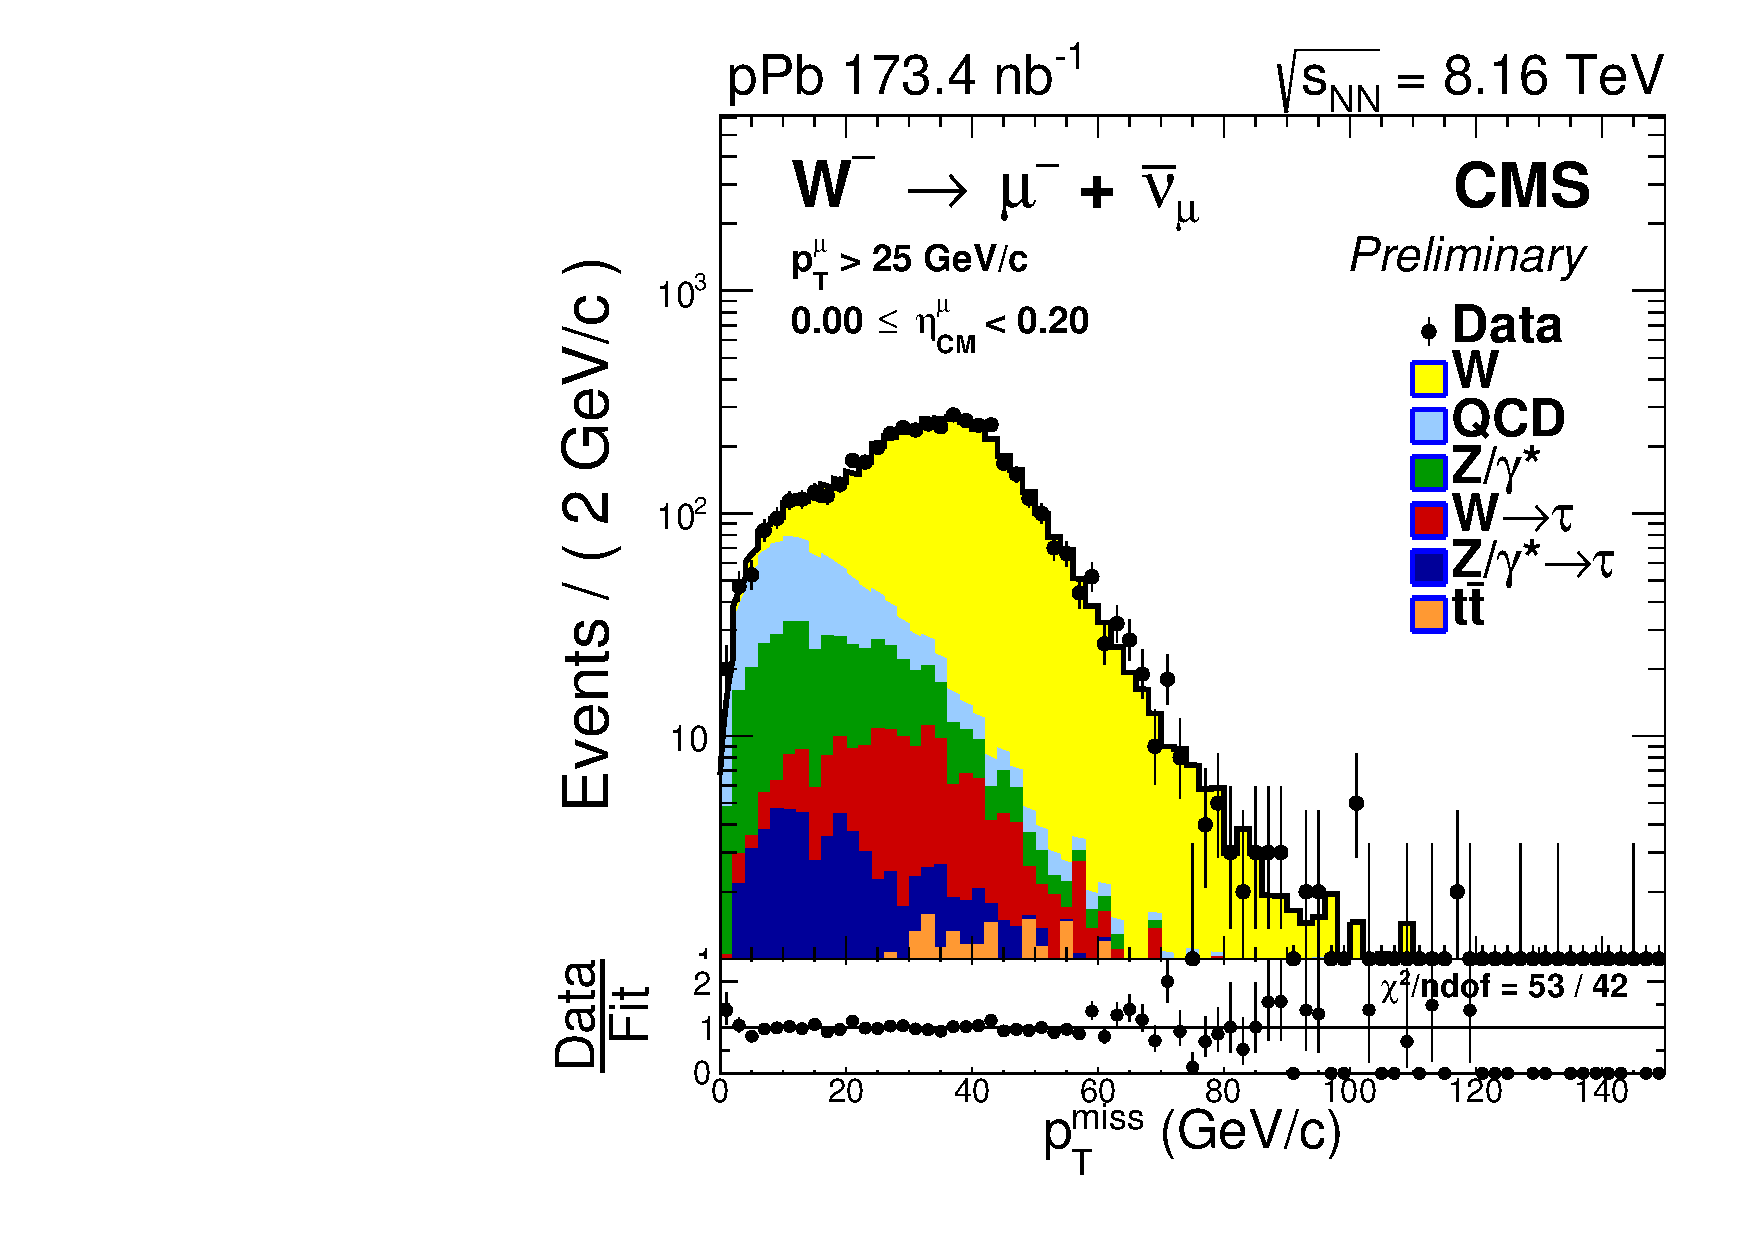
\includegraphics[width=0.23\textwidth]{Figures/WBoson/Analysis/SignalExtraction/Signal/LOG/PLOT_MET_DATA_WToMuMi_PA_Model_TEMP_WDYDYToTauWToTauTTbar_ModifiedRayleigh_QCD_MuEtaCM_0_20_MuIso_0_15.pdf}
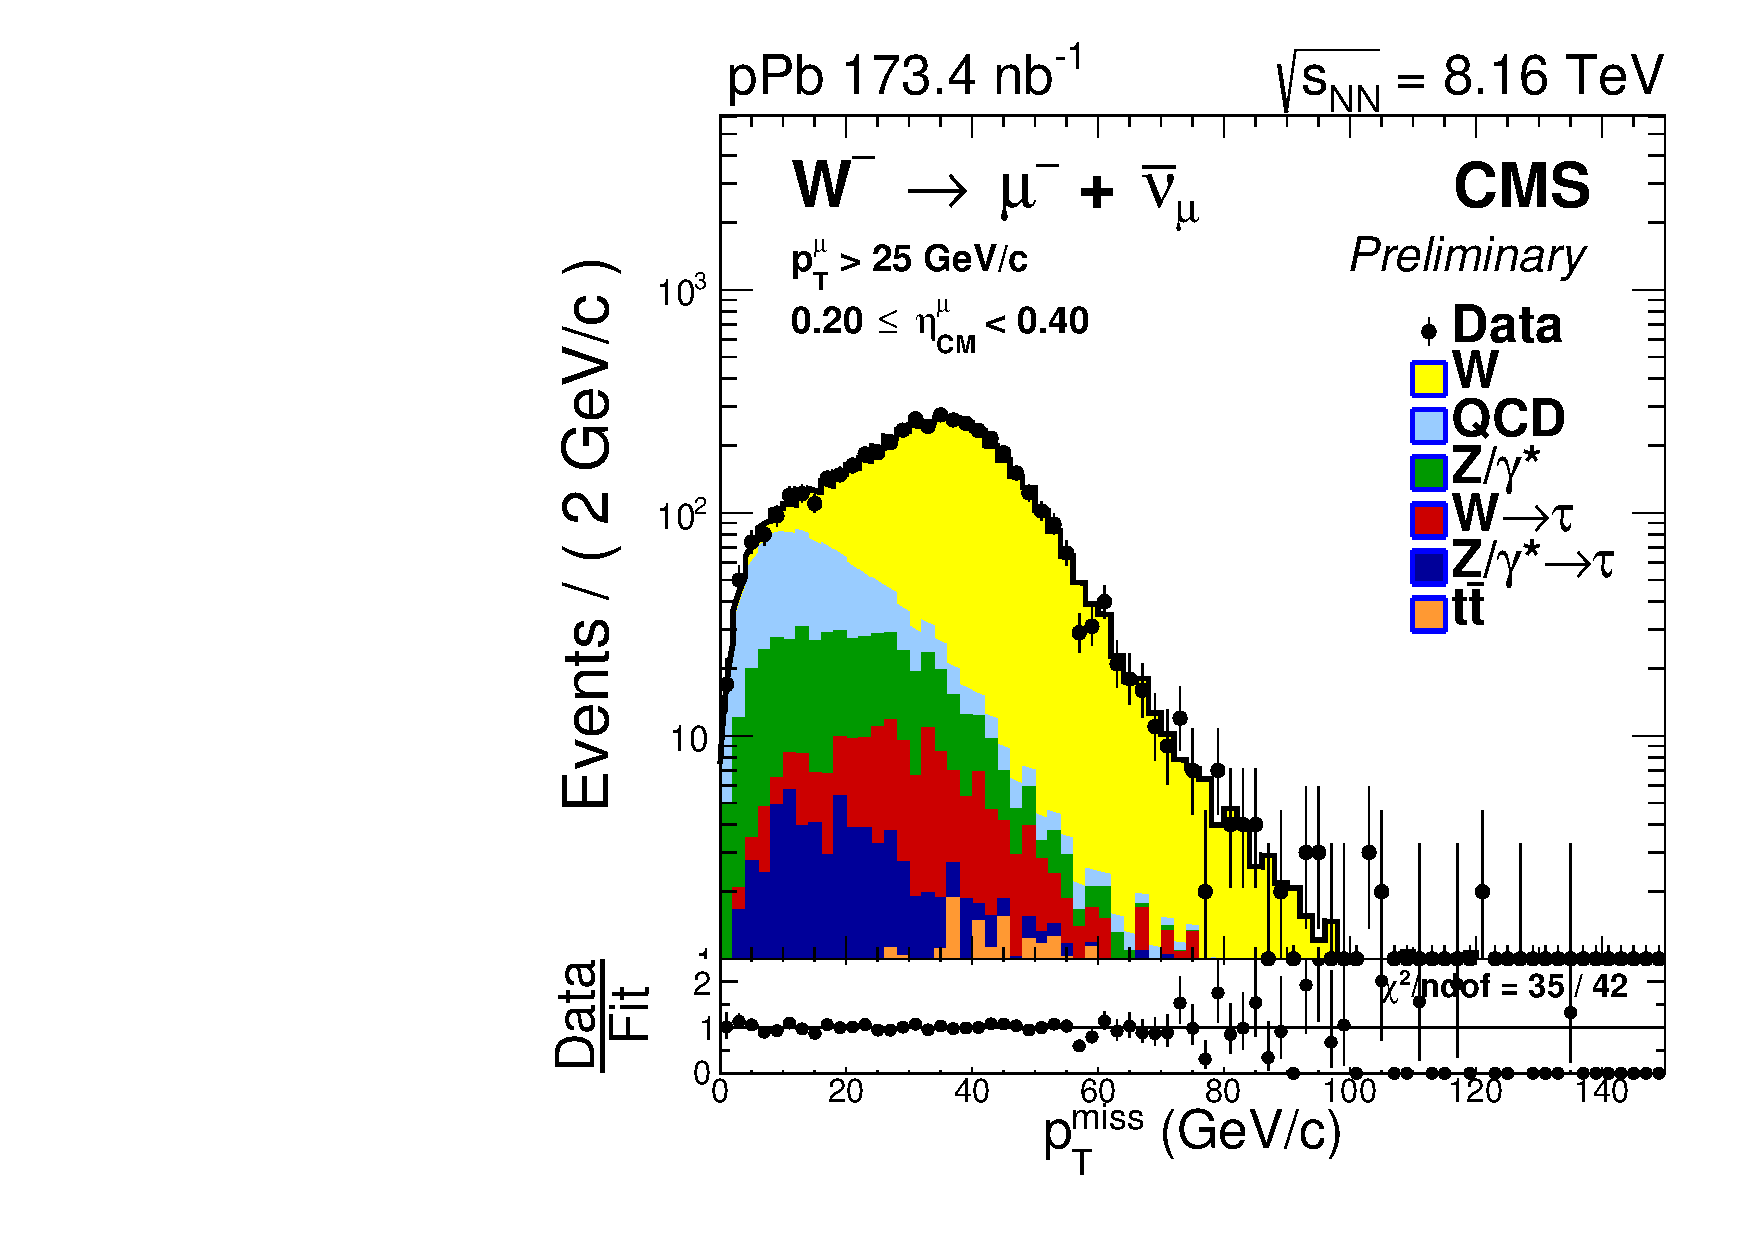
\includegraphics[width=0.23\textwidth]{Figures/WBoson/Analysis/SignalExtraction/Signal/LOG/PLOT_MET_DATA_WToMuMi_PA_Model_TEMP_WDYDYToTauWToTauTTbar_ModifiedRayleigh_QCD_MuEtaCM_20_40_MuIso_0_15.pdf}
\\
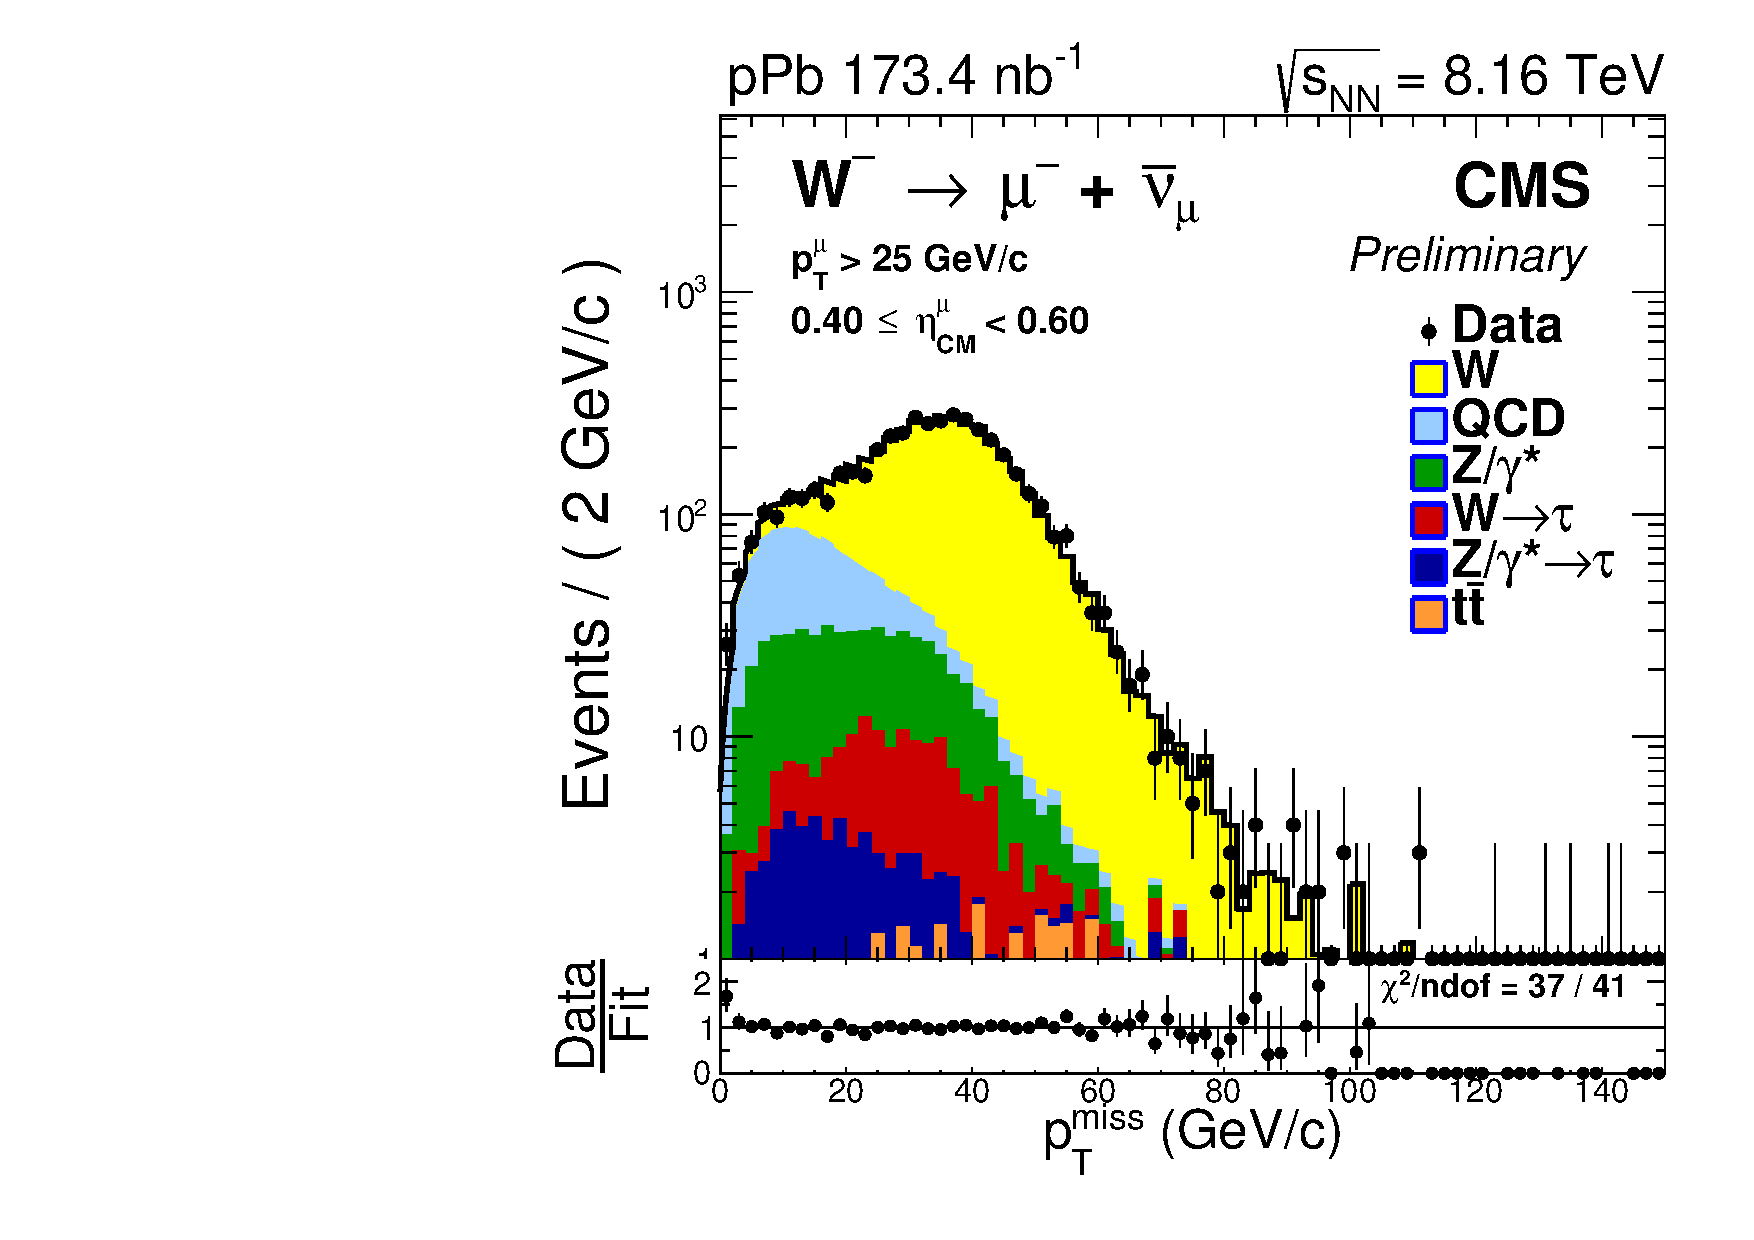
\includegraphics[width=0.23\textwidth]{Figures/WBoson/Analysis/SignalExtraction/Signal/LOG/PLOT_MET_DATA_WToMuMi_PA_Model_TEMP_WDYDYToTauWToTauTTbar_ModifiedRayleigh_QCD_MuEtaCM_40_60_MuIso_0_15.pdf}
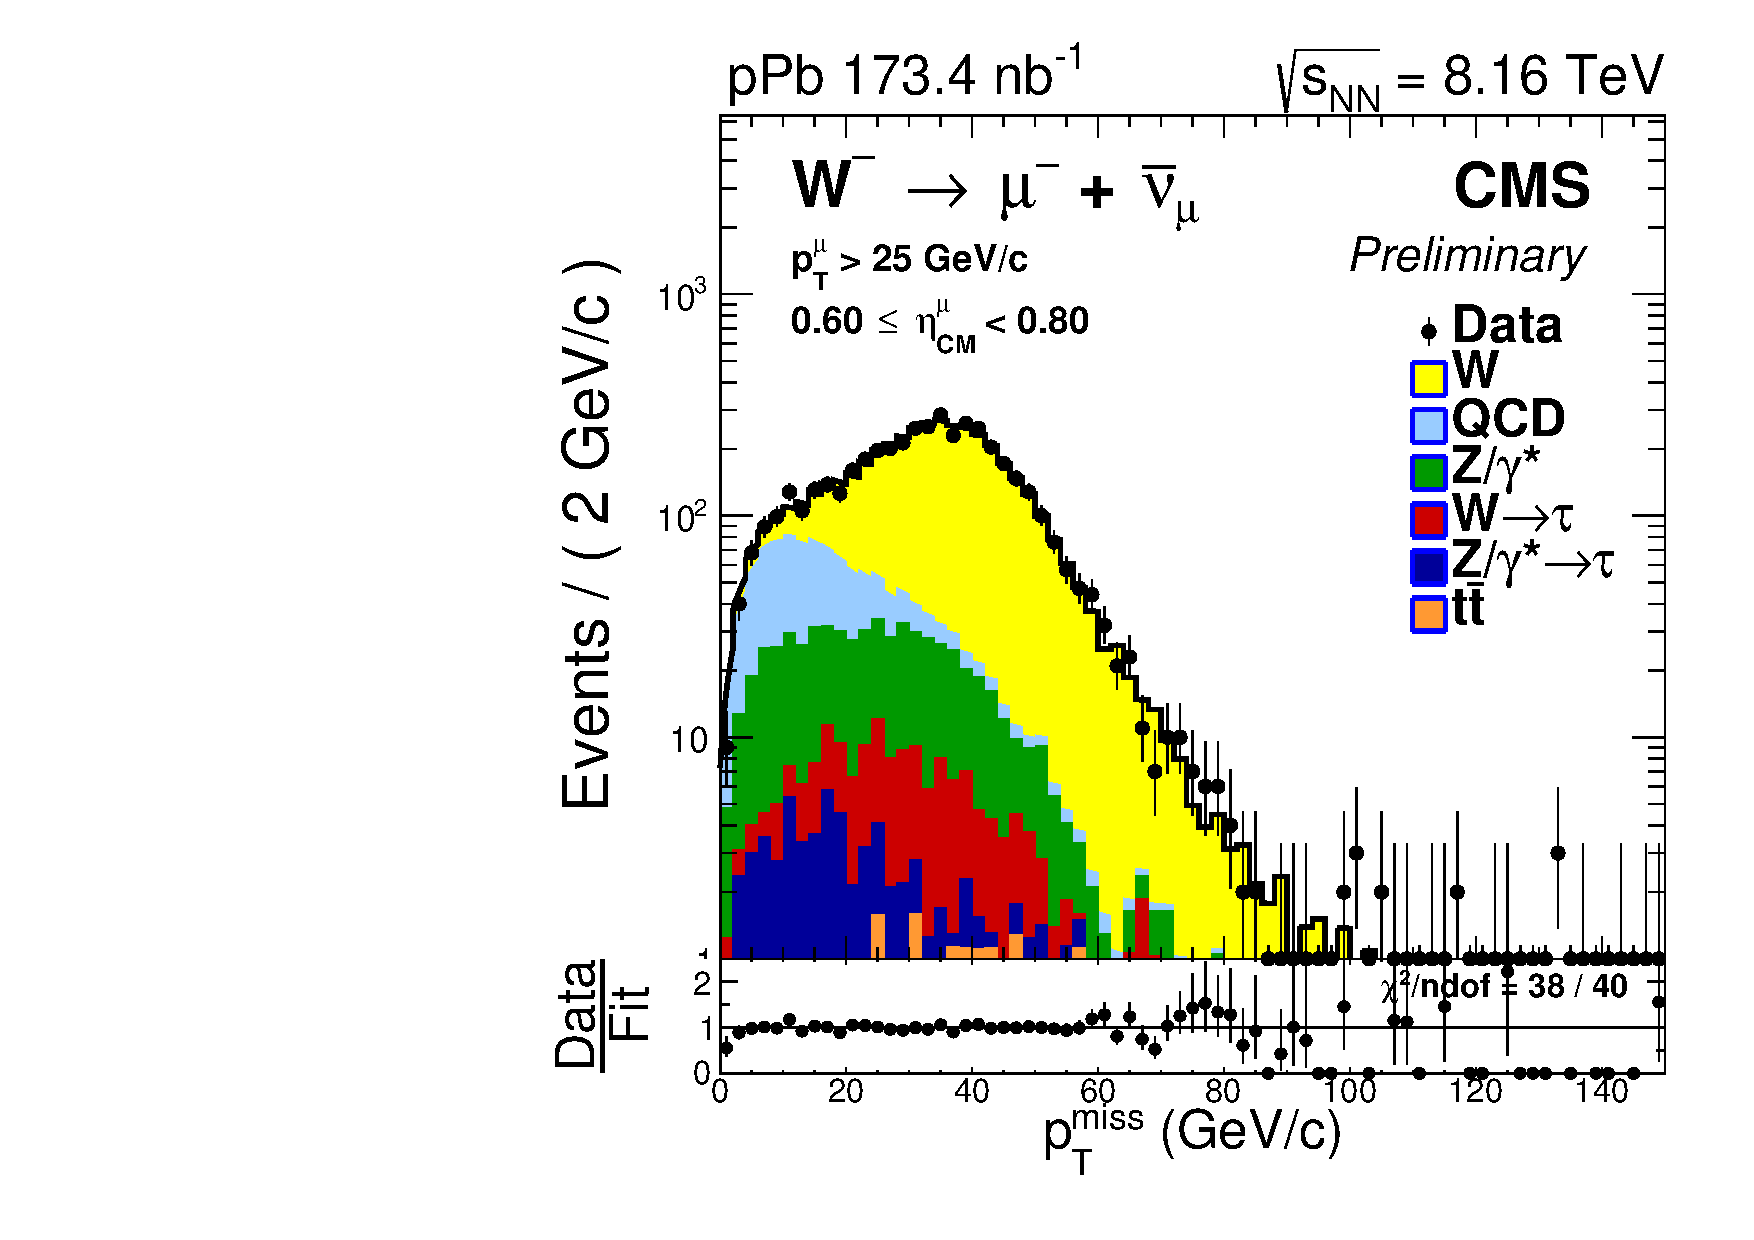
\includegraphics[width=0.23\textwidth]{Figures/WBoson/Analysis/SignalExtraction/Signal/LOG/PLOT_MET_DATA_WToMuMi_PA_Model_TEMP_WDYDYToTauWToTauTTbar_ModifiedRayleigh_QCD_MuEtaCM_60_80_MuIso_0_15.pdf}
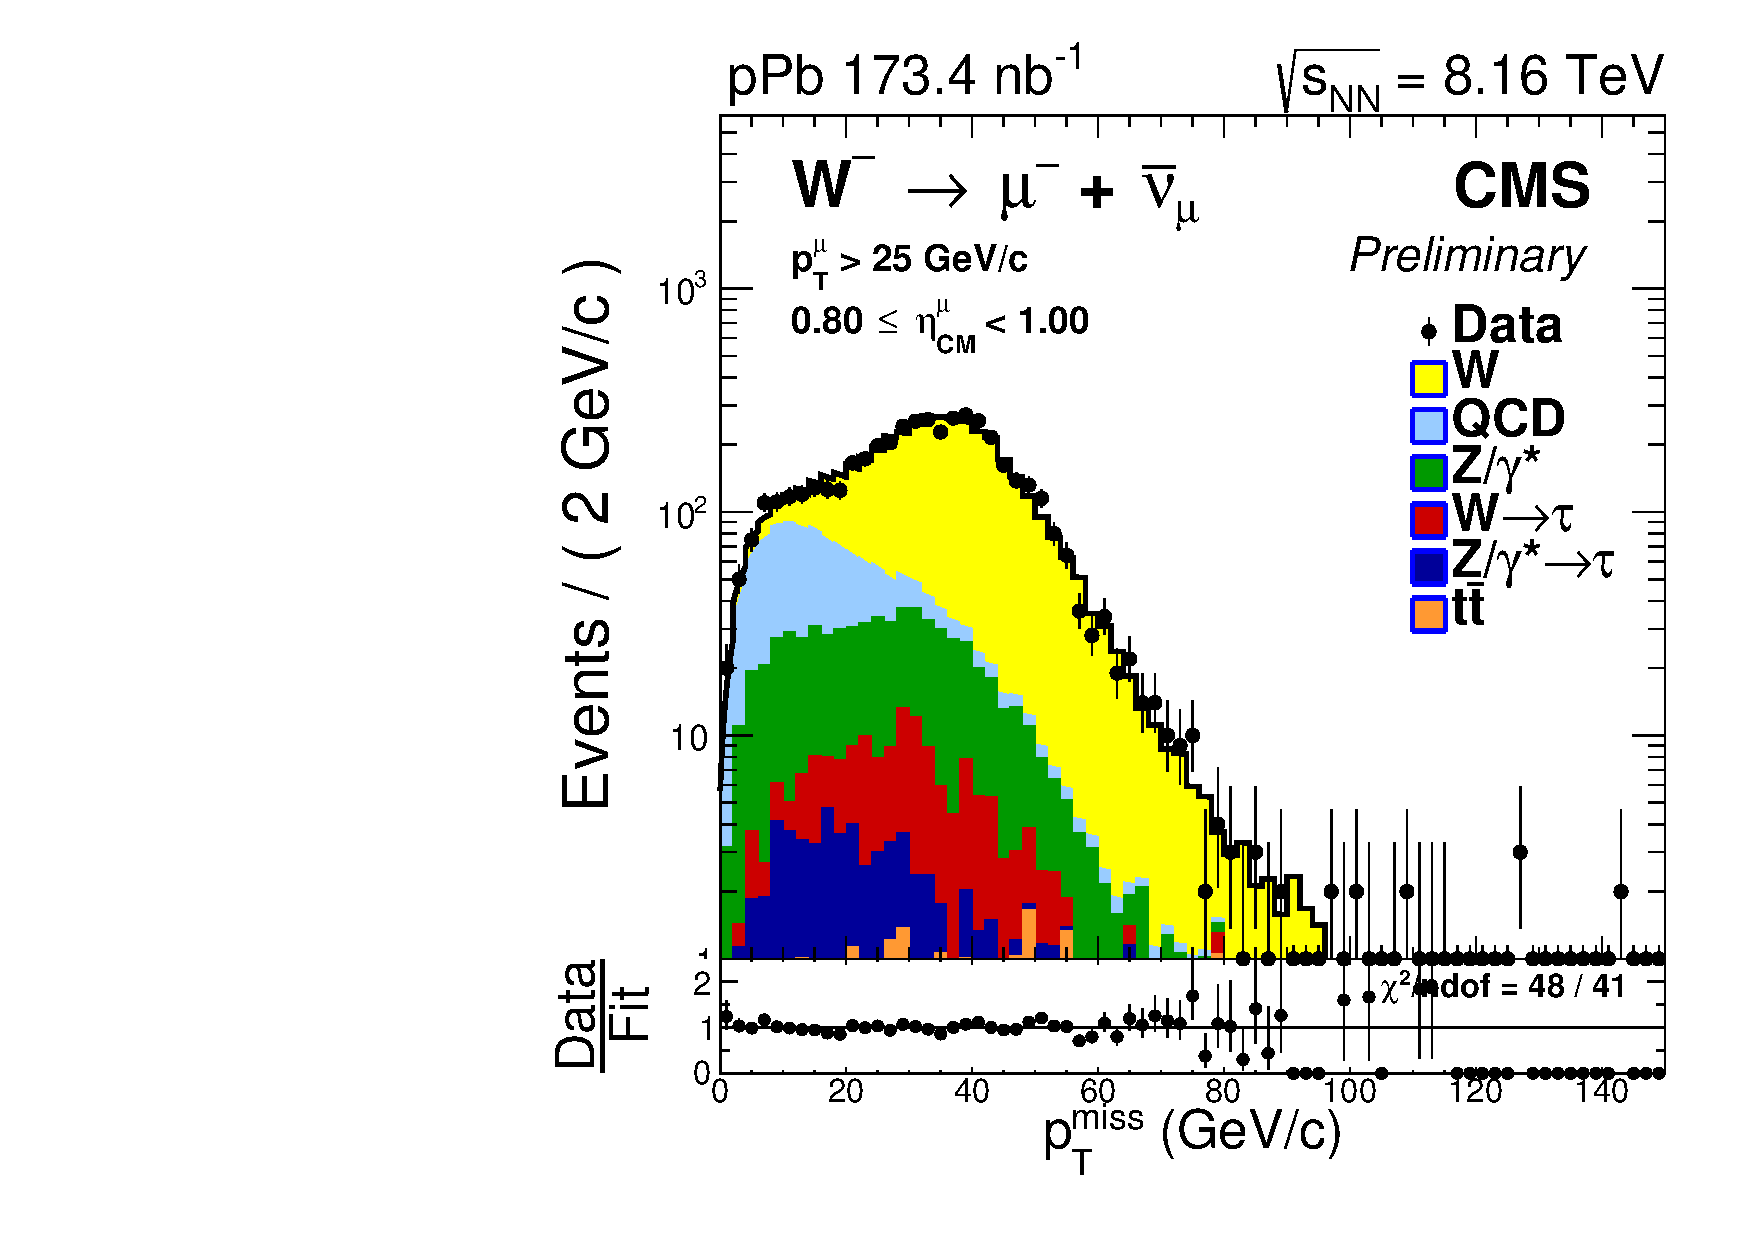
\includegraphics[width=0.23\textwidth]{Figures/WBoson/Analysis/SignalExtraction/Signal/LOG/PLOT_MET_DATA_WToMuMi_PA_Model_TEMP_WDYDYToTauWToTauTTbar_ModifiedRayleigh_QCD_MuEtaCM_80_100_MuIso_0_15.pdf}
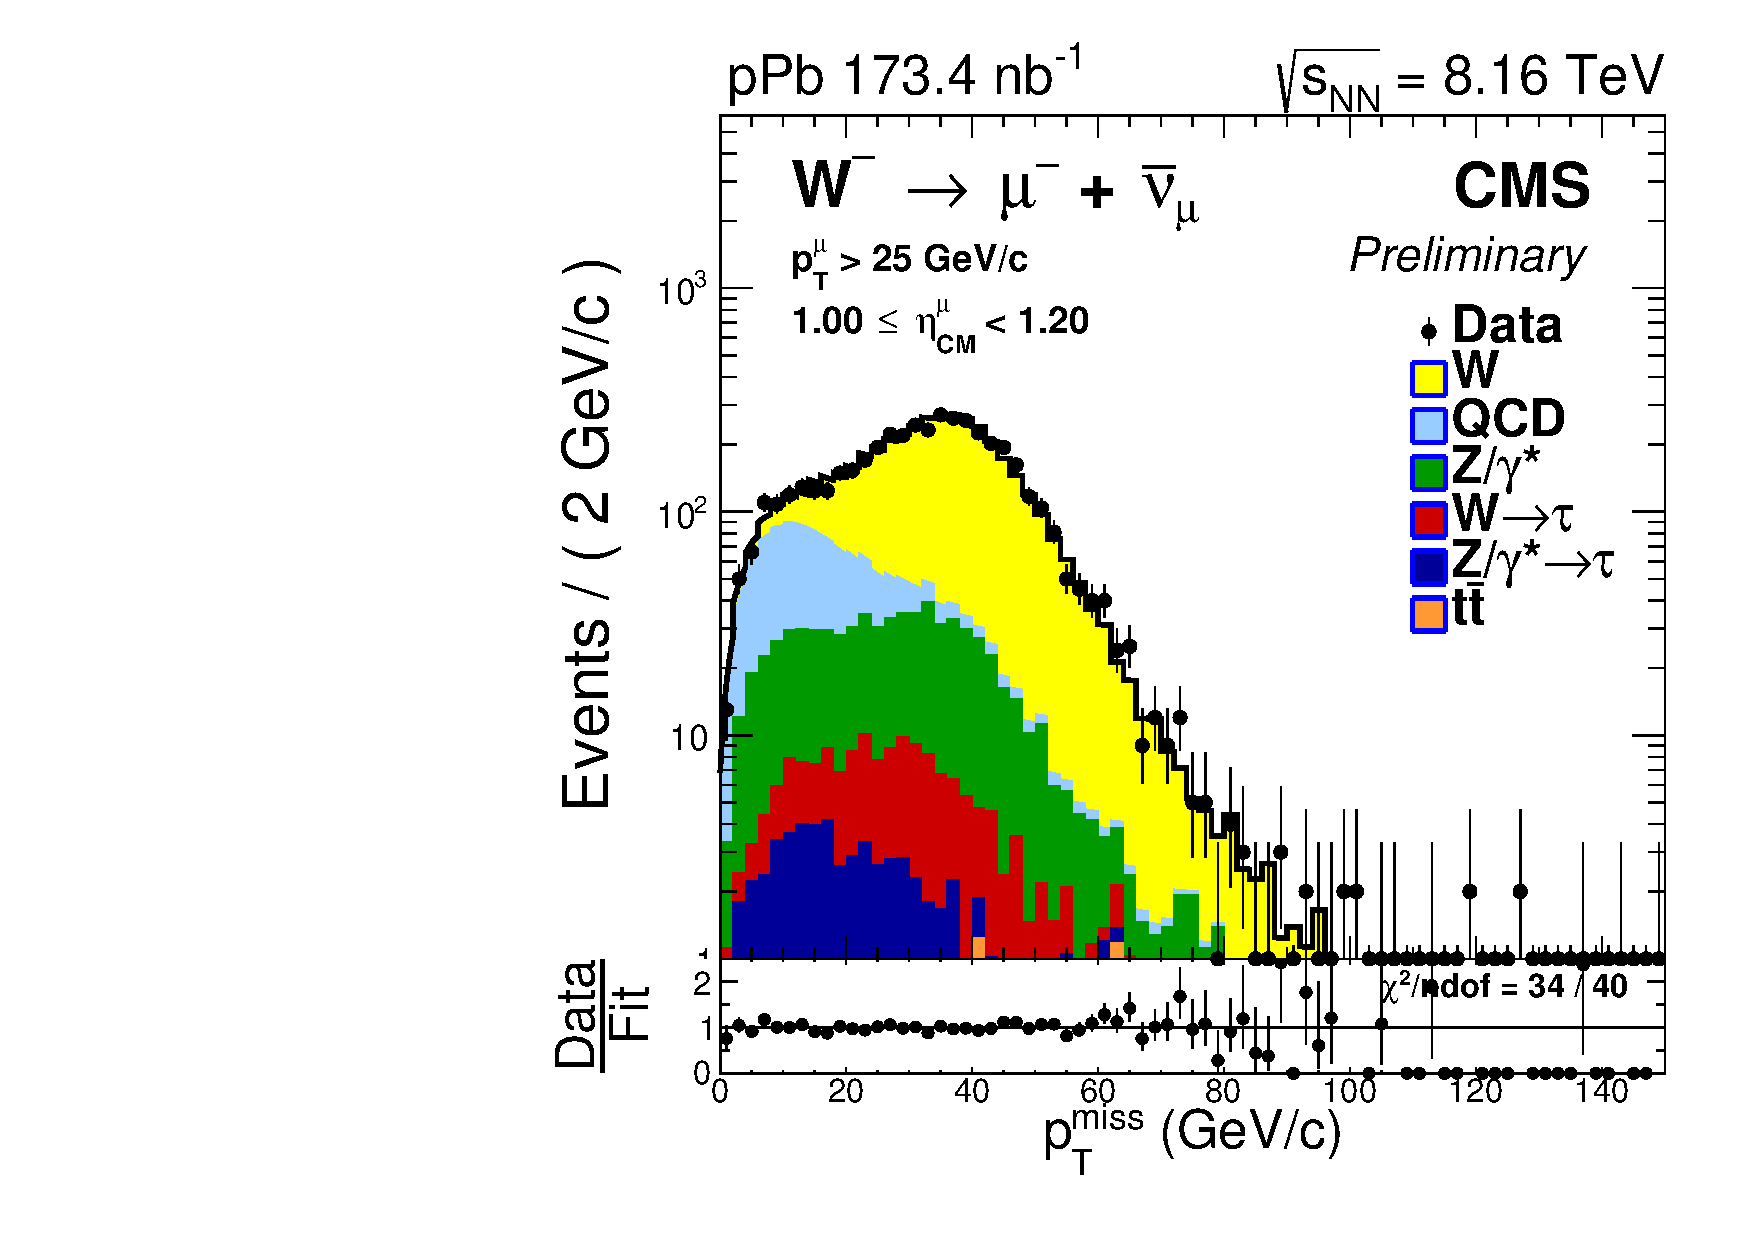
\includegraphics[width=0.23\textwidth]{Figures/WBoson/Analysis/SignalExtraction/Signal/LOG/PLOT_MET_DATA_WToMuMi_PA_Model_TEMP_WDYDYToTauWToTauTTbar_ModifiedRayleigh_QCD_MuEtaCM_100_120_MuIso_0_15.pdf}
\\
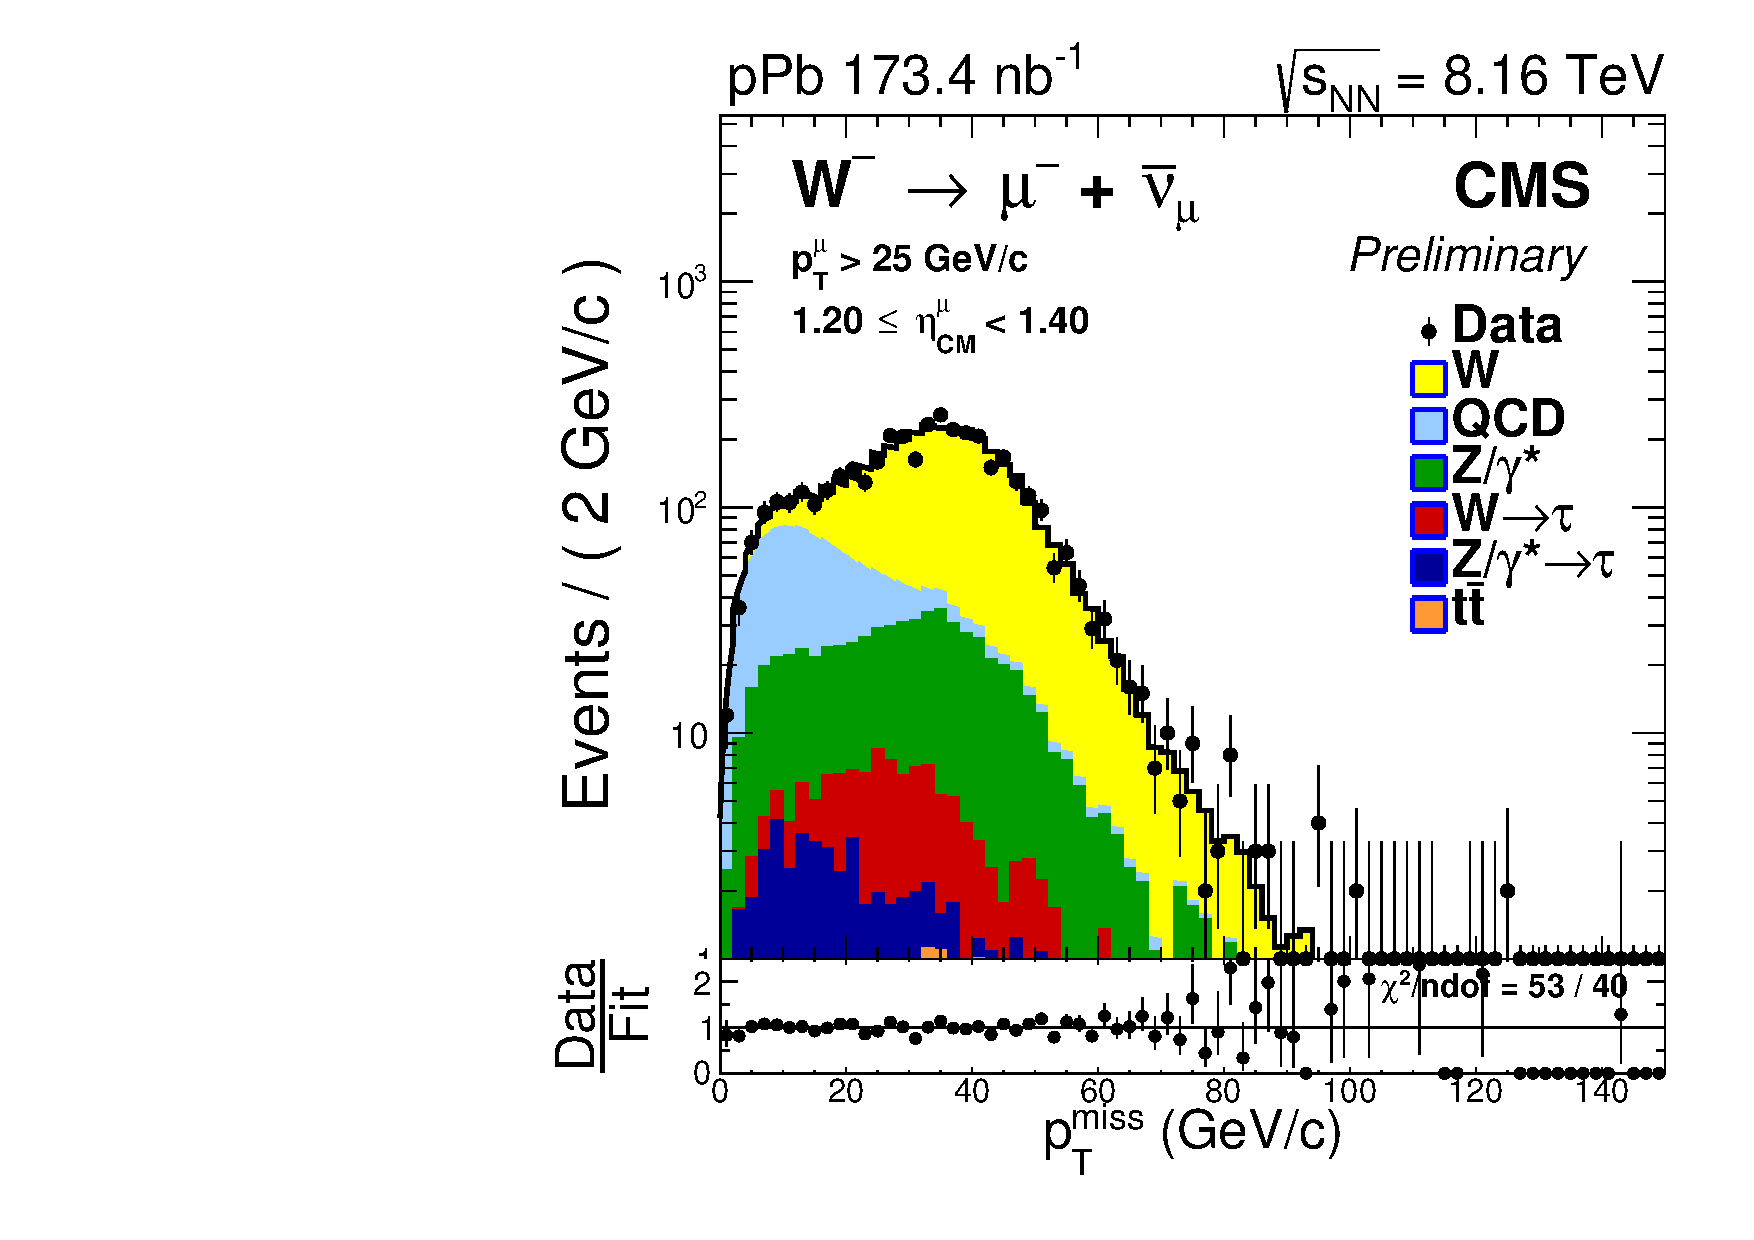
\includegraphics[width=0.23\textwidth]{Figures/WBoson/Analysis/SignalExtraction/Signal/LOG/PLOT_MET_DATA_WToMuMi_PA_Model_TEMP_WDYDYToTauWToTauTTbar_ModifiedRayleigh_QCD_MuEtaCM_120_140_MuIso_0_15.pdf}
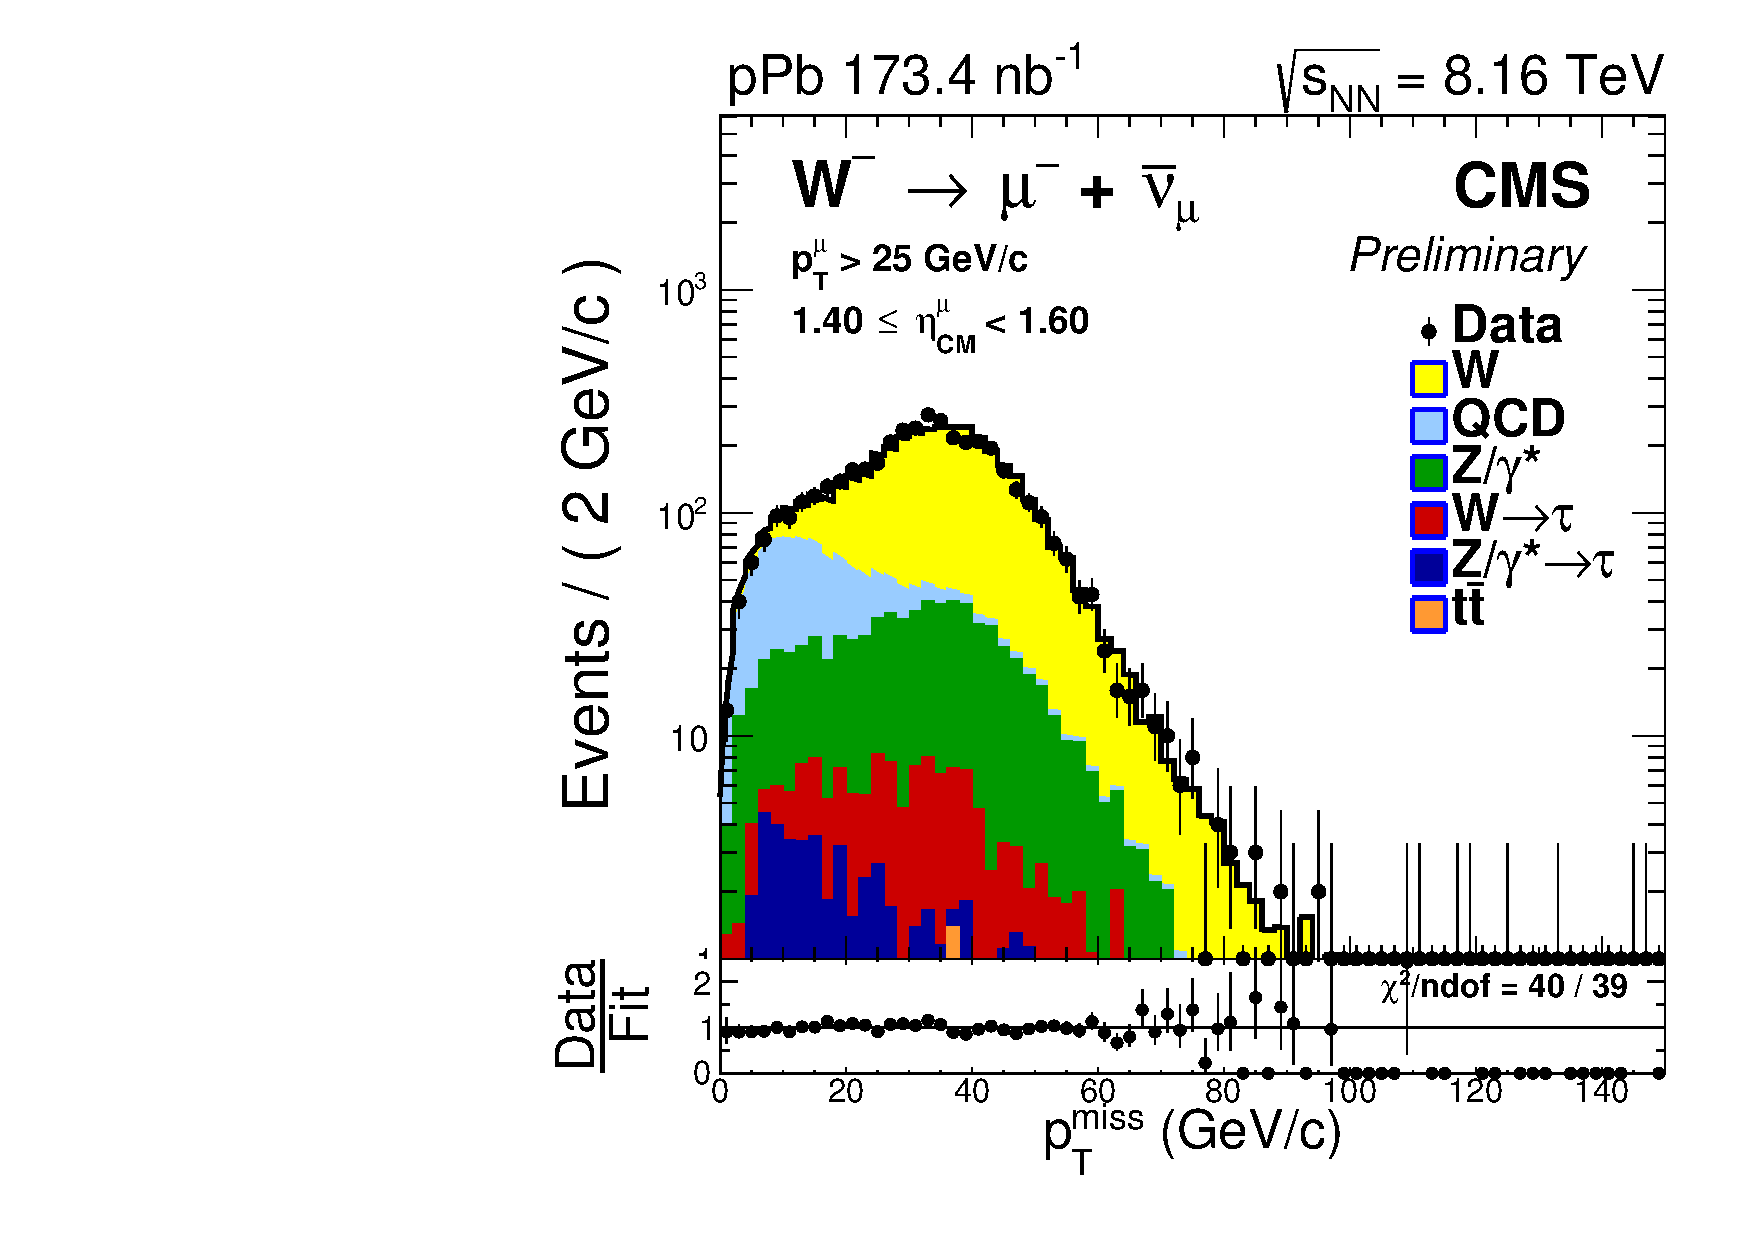
\includegraphics[width=0.23\textwidth]{Figures/WBoson/Analysis/SignalExtraction/Signal/LOG/PLOT_MET_DATA_WToMuMi_PA_Model_TEMP_WDYDYToTauWToTauTTbar_ModifiedRayleigh_QCD_MuEtaCM_140_160_MuIso_0_15.pdf}
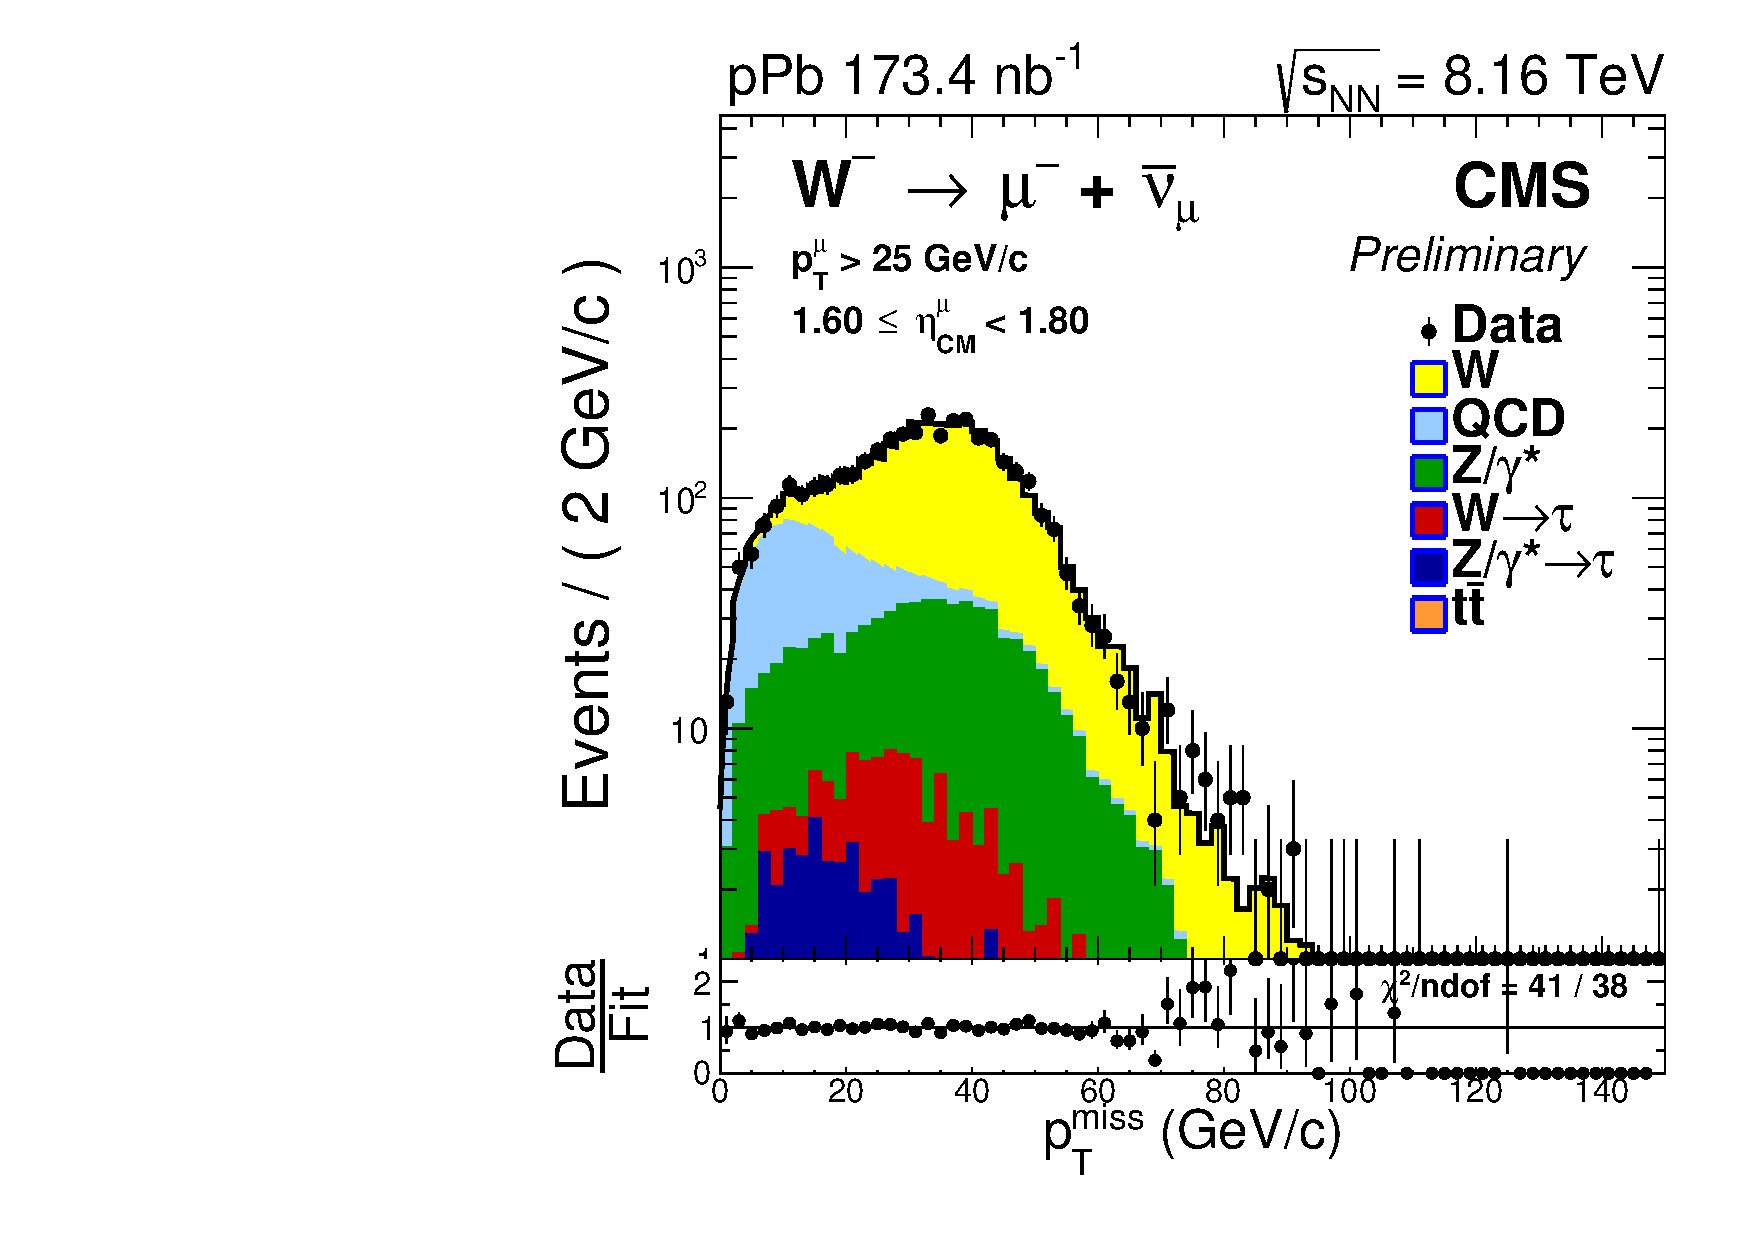
\includegraphics[width=0.23\textwidth]{Figures/WBoson/Analysis/SignalExtraction/Signal/LOG/PLOT_MET_DATA_WToMuMi_PA_Model_TEMP_WDYDYToTauWToTauTTbar_ModifiedRayleigh_QCD_MuEtaCM_160_180_MuIso_0_15.pdf}
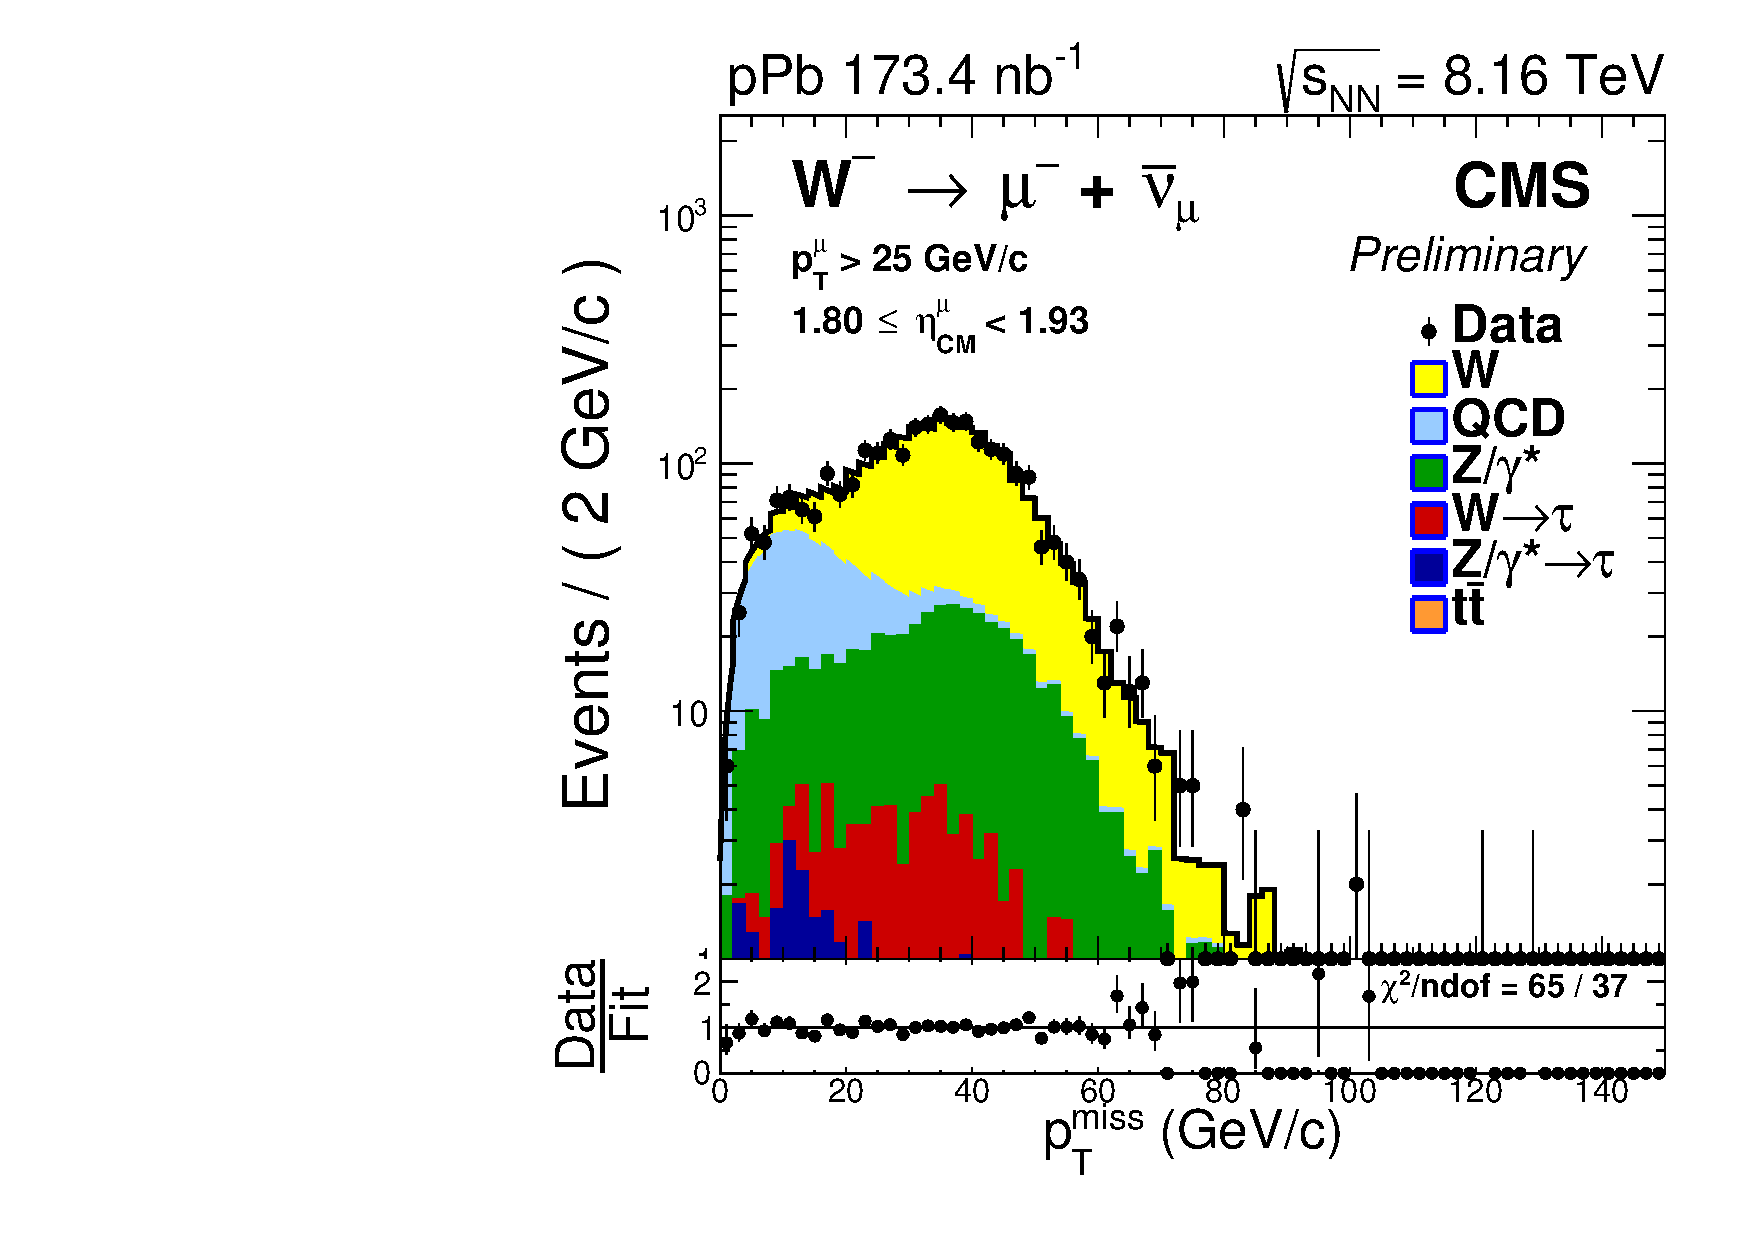
\includegraphics[width=0.23\textwidth]{Figures/WBoson/Analysis/SignalExtraction/Signal/LOG/PLOT_MET_DATA_WToMuMi_PA_Model_TEMP_WDYDYToTauWToTauTTbar_ModifiedRayleigh_QCD_MuEtaCM_180_193_MuIso_0_15.pdf}
\end{tiny}
\caption{The \ptmiss distribution for \WToMuNuMi events within each fitted \etaMuCM range, shown in logarithmic scale. Unbinned fits to the data (black points) are performed with six contributions, stacked from top to bottom: \WToMuNuPl (yellow), QCD multijet (light blue), \DYToMuMu (green), \WToTauNuPl (red), \DYToTauTau (dark blue) and \ttbar (orange). Error bars represent statistical uncertainties. The lower panels display the data divided by the result of the fit, for each \etaMuCM range. The $\chi^{2}$ test value over the number of degrees of freedom is also shown.}
\label{fig:METFits_WToMuMi_PA}
 
\end{figure}


\begin{figure}[htb!]
\centering
\begin{tiny}
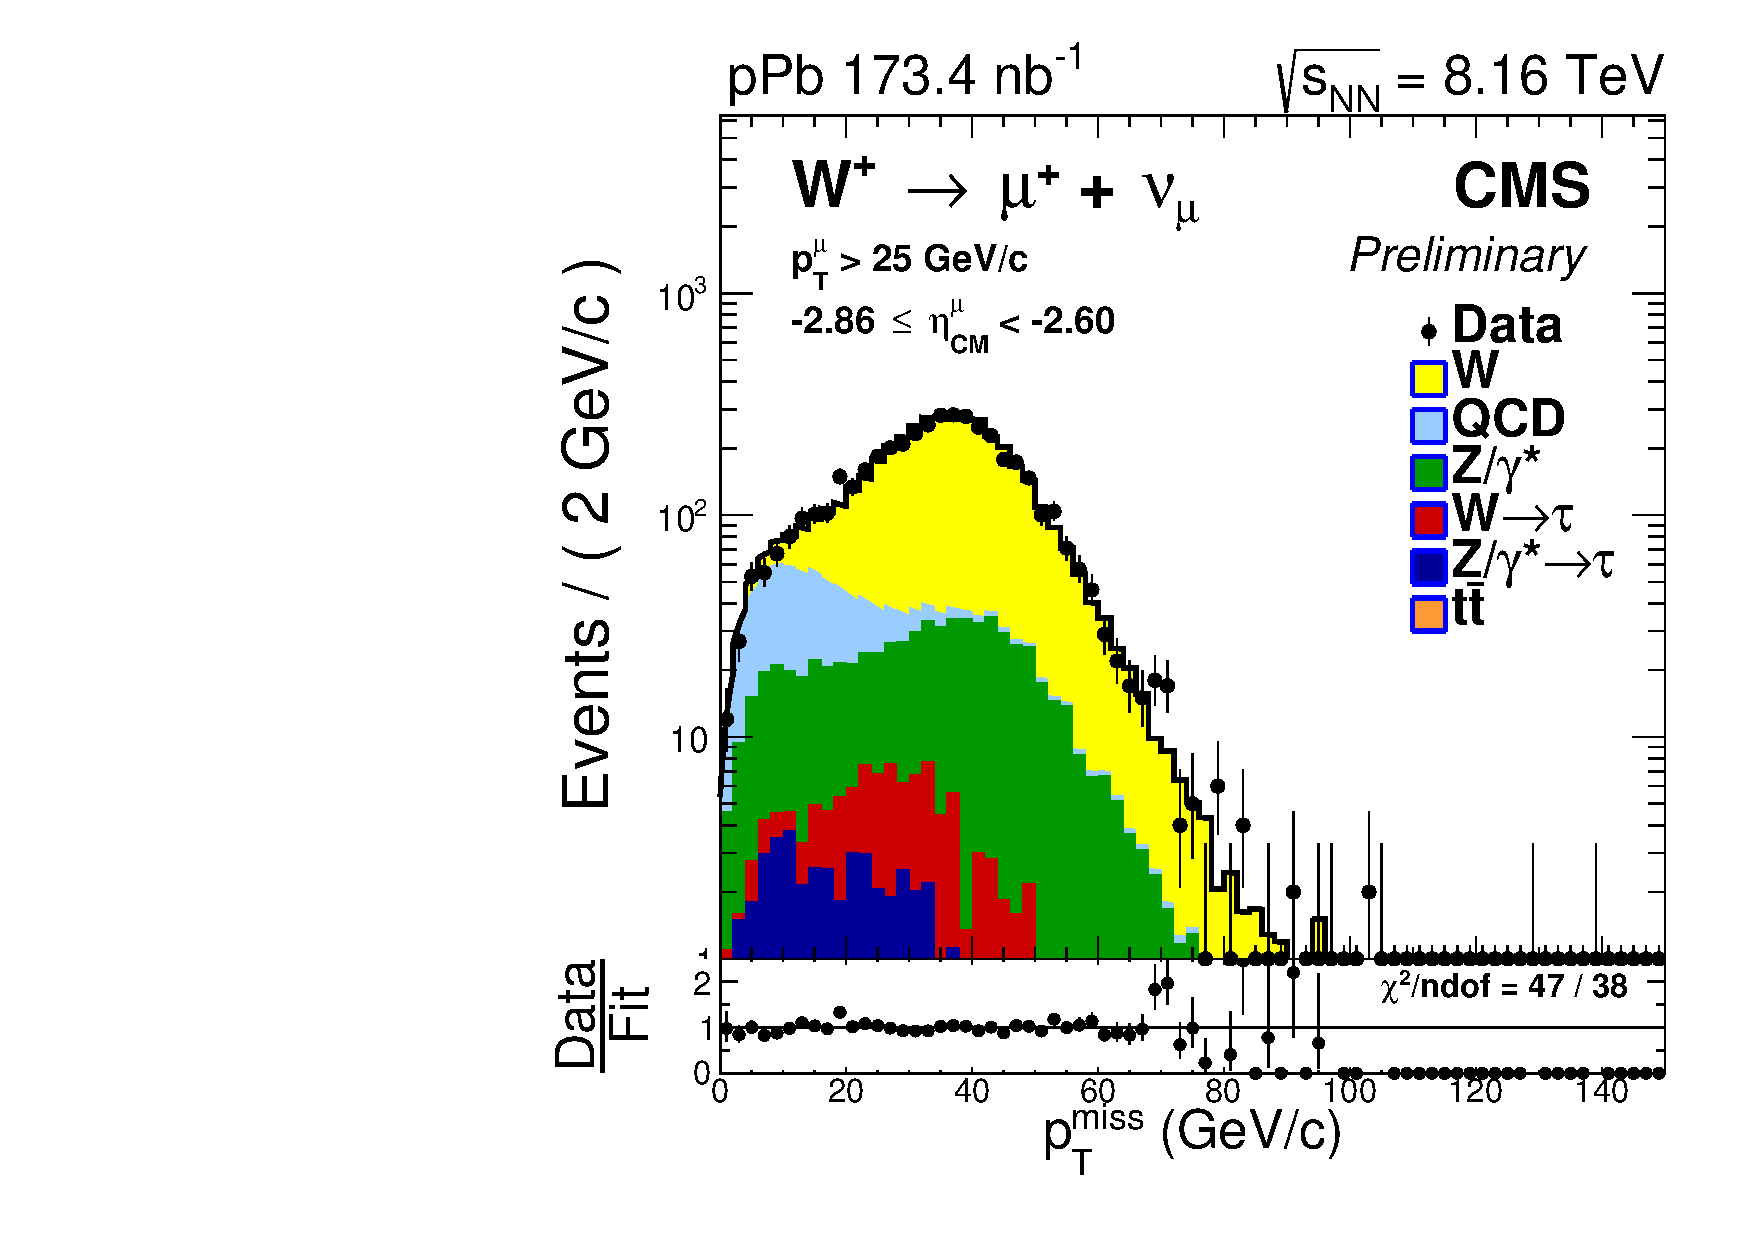
\includegraphics[width=0.23\textwidth]{Figures/WBoson/Analysis/SignalExtraction/Signal/LOG/PLOT_MET_DATA_WToMuPl_PA_Model_TEMP_WDYDYToTauWToTauTTbar_ModifiedRayleigh_QCD_MuEtaCM_-286_-260_MuIso_0_15.pdf}
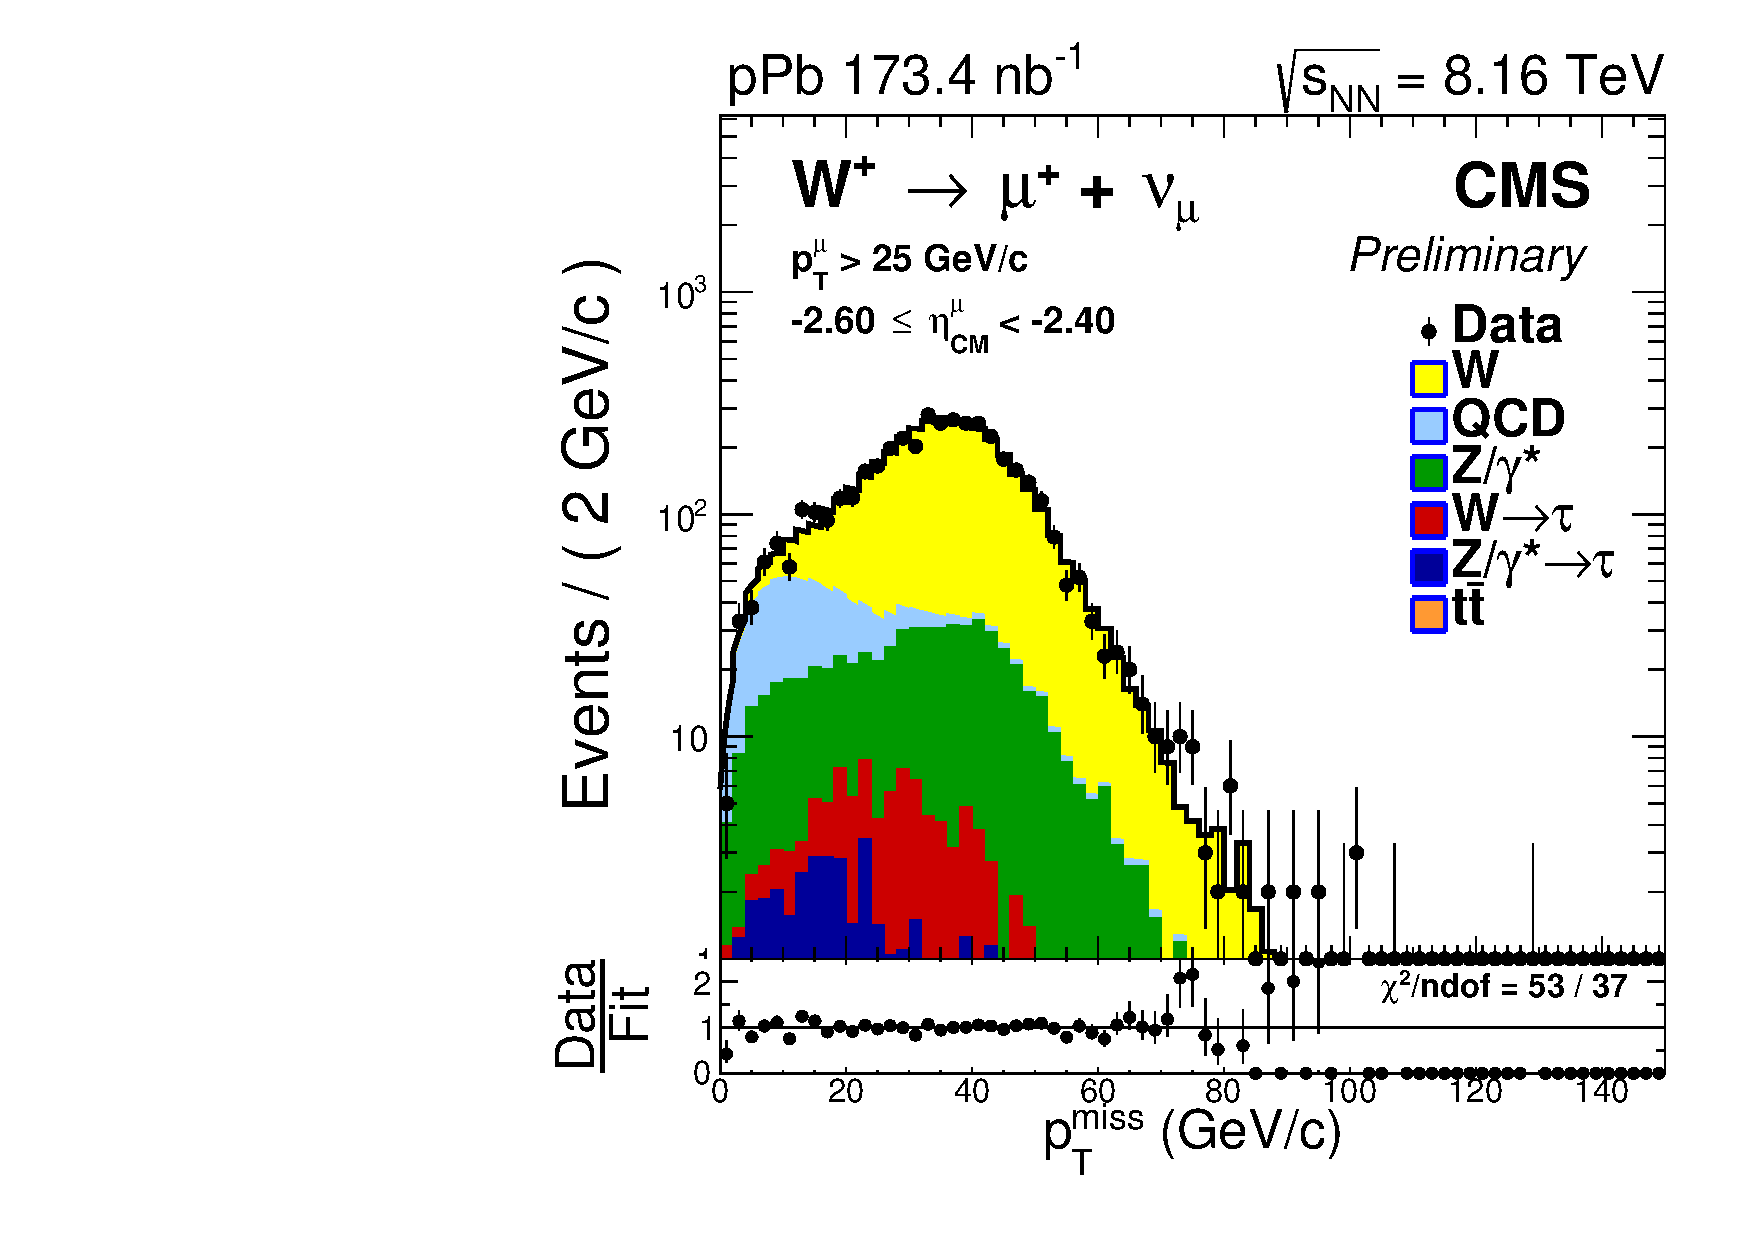
\includegraphics[width=0.23\textwidth]{Figures/WBoson/Analysis/SignalExtraction/Signal/LOG/PLOT_MET_DATA_WToMuPl_PA_Model_TEMP_WDYDYToTauWToTauTTbar_ModifiedRayleigh_QCD_MuEtaCM_-260_-240_MuIso_0_15.pdf}
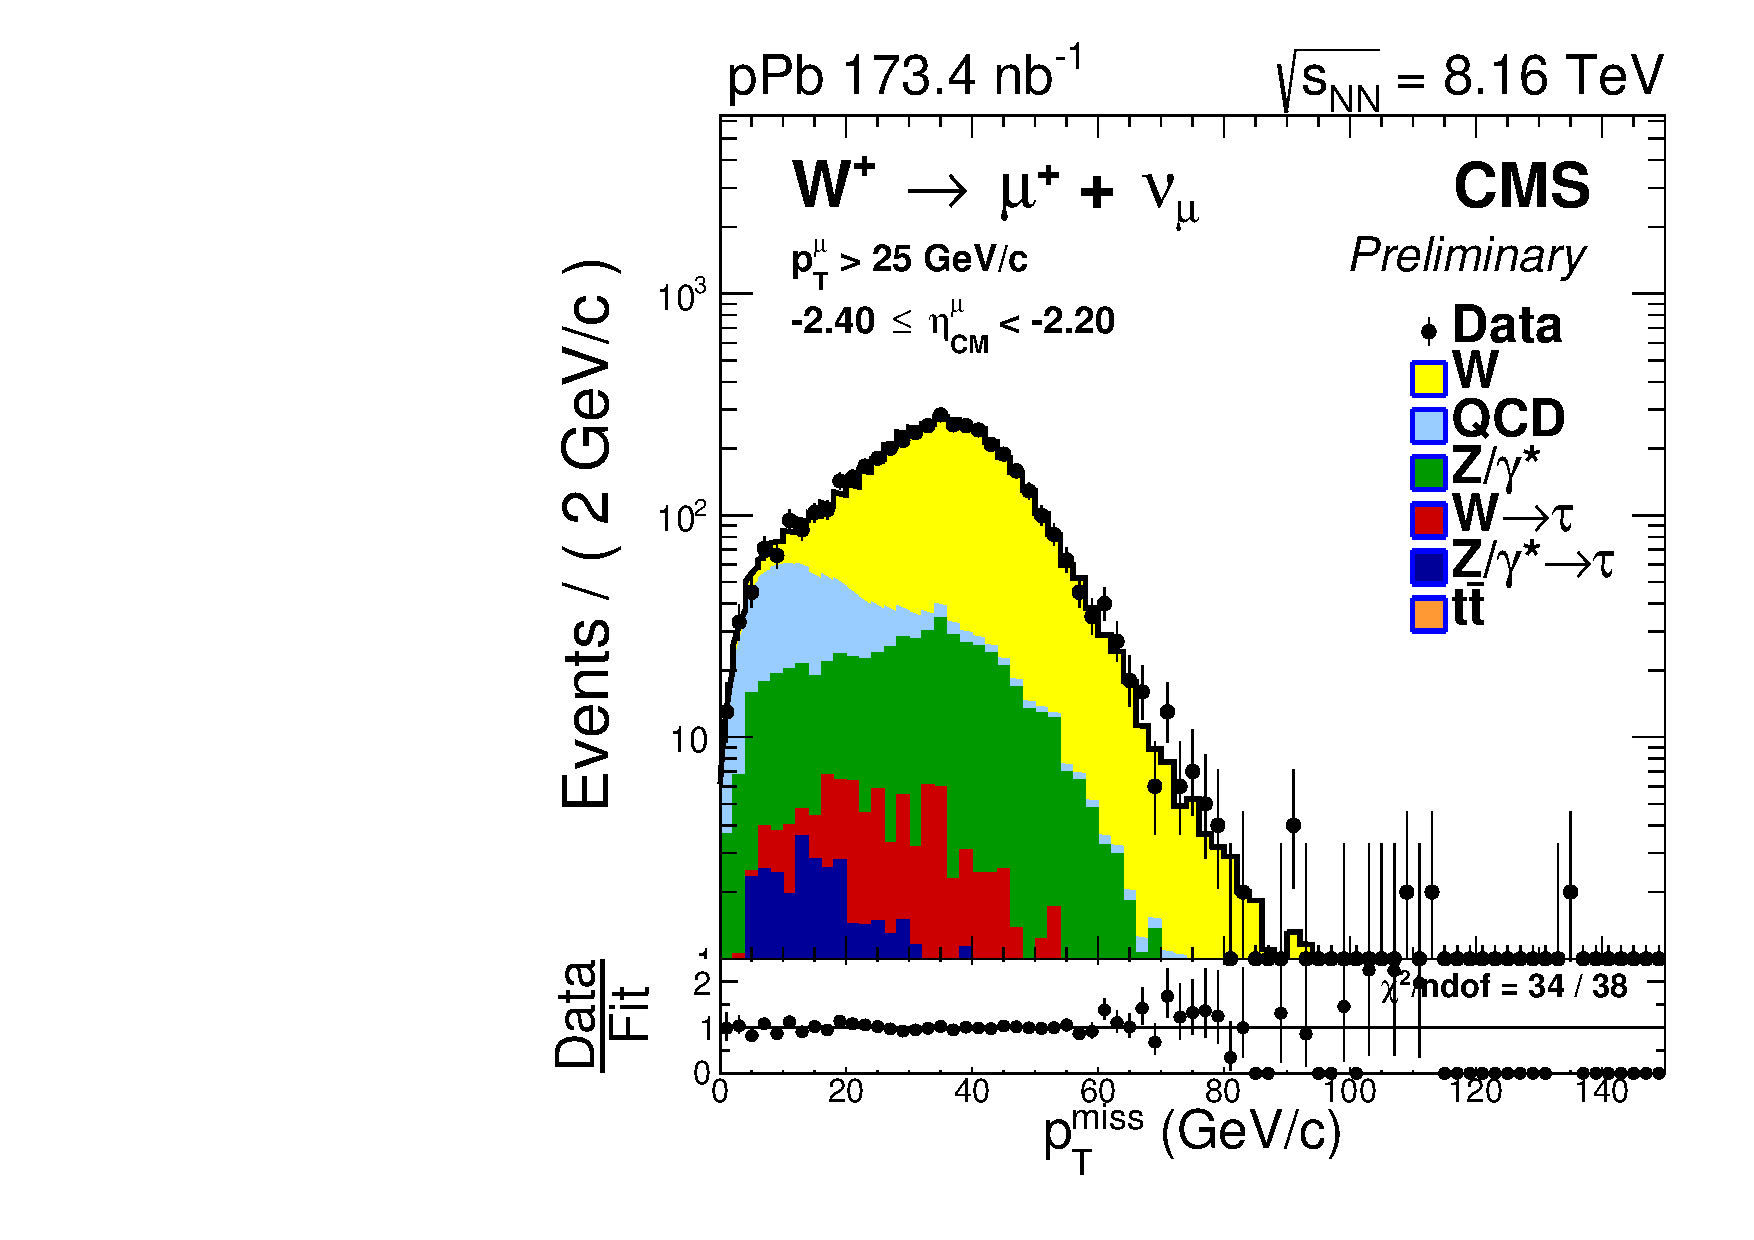
\includegraphics[width=0.23\textwidth]{Figures/WBoson/Analysis/SignalExtraction/Signal/LOG/PLOT_MET_DATA_WToMuPl_PA_Model_TEMP_WDYDYToTauWToTauTTbar_ModifiedRayleigh_QCD_MuEtaCM_-240_-220_MuIso_0_15.pdf}
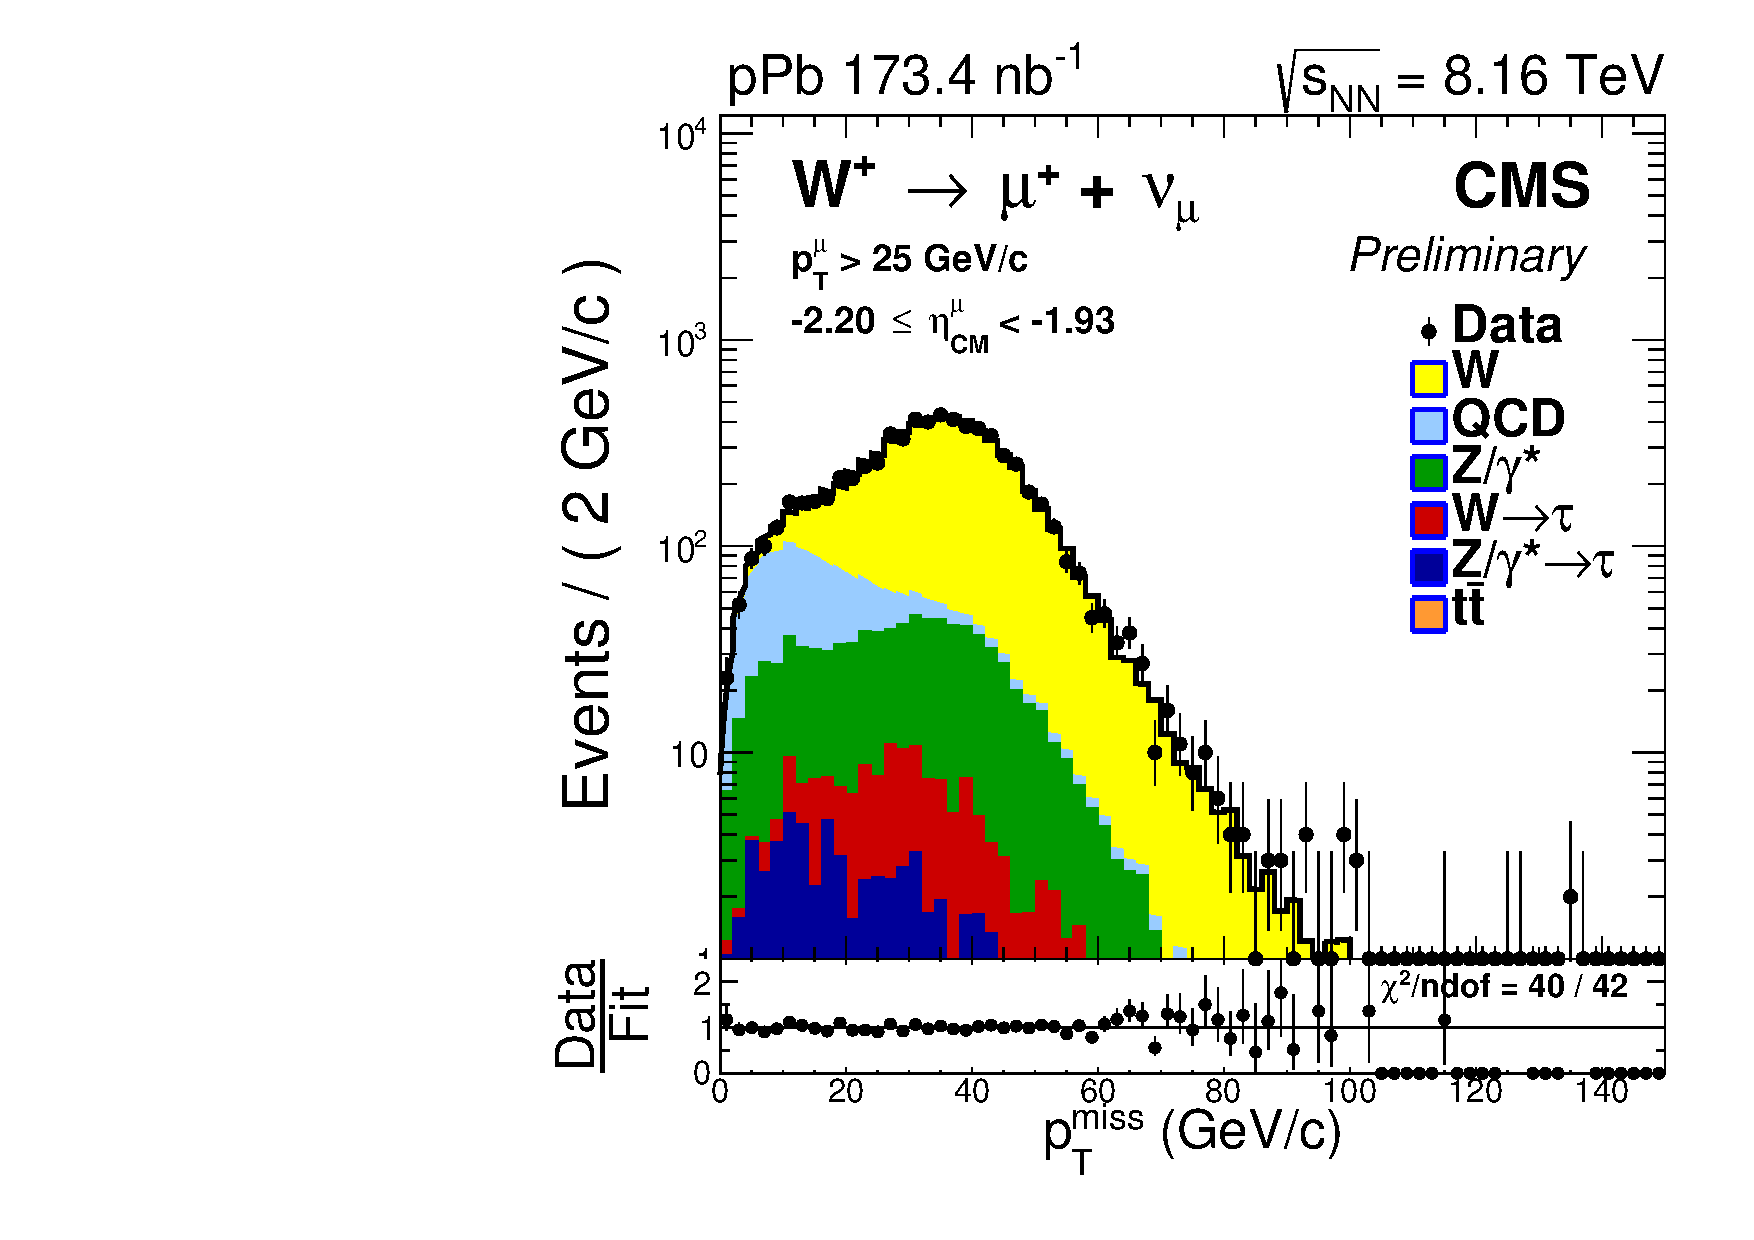
\includegraphics[width=0.23\textwidth]{Figures/WBoson/Analysis/SignalExtraction/Signal/LOG/PLOT_MET_DATA_WToMuPl_PA_Model_TEMP_WDYDYToTauWToTauTTbar_ModifiedRayleigh_QCD_MuEtaCM_-220_-193_MuIso_0_15.pdf}
\\
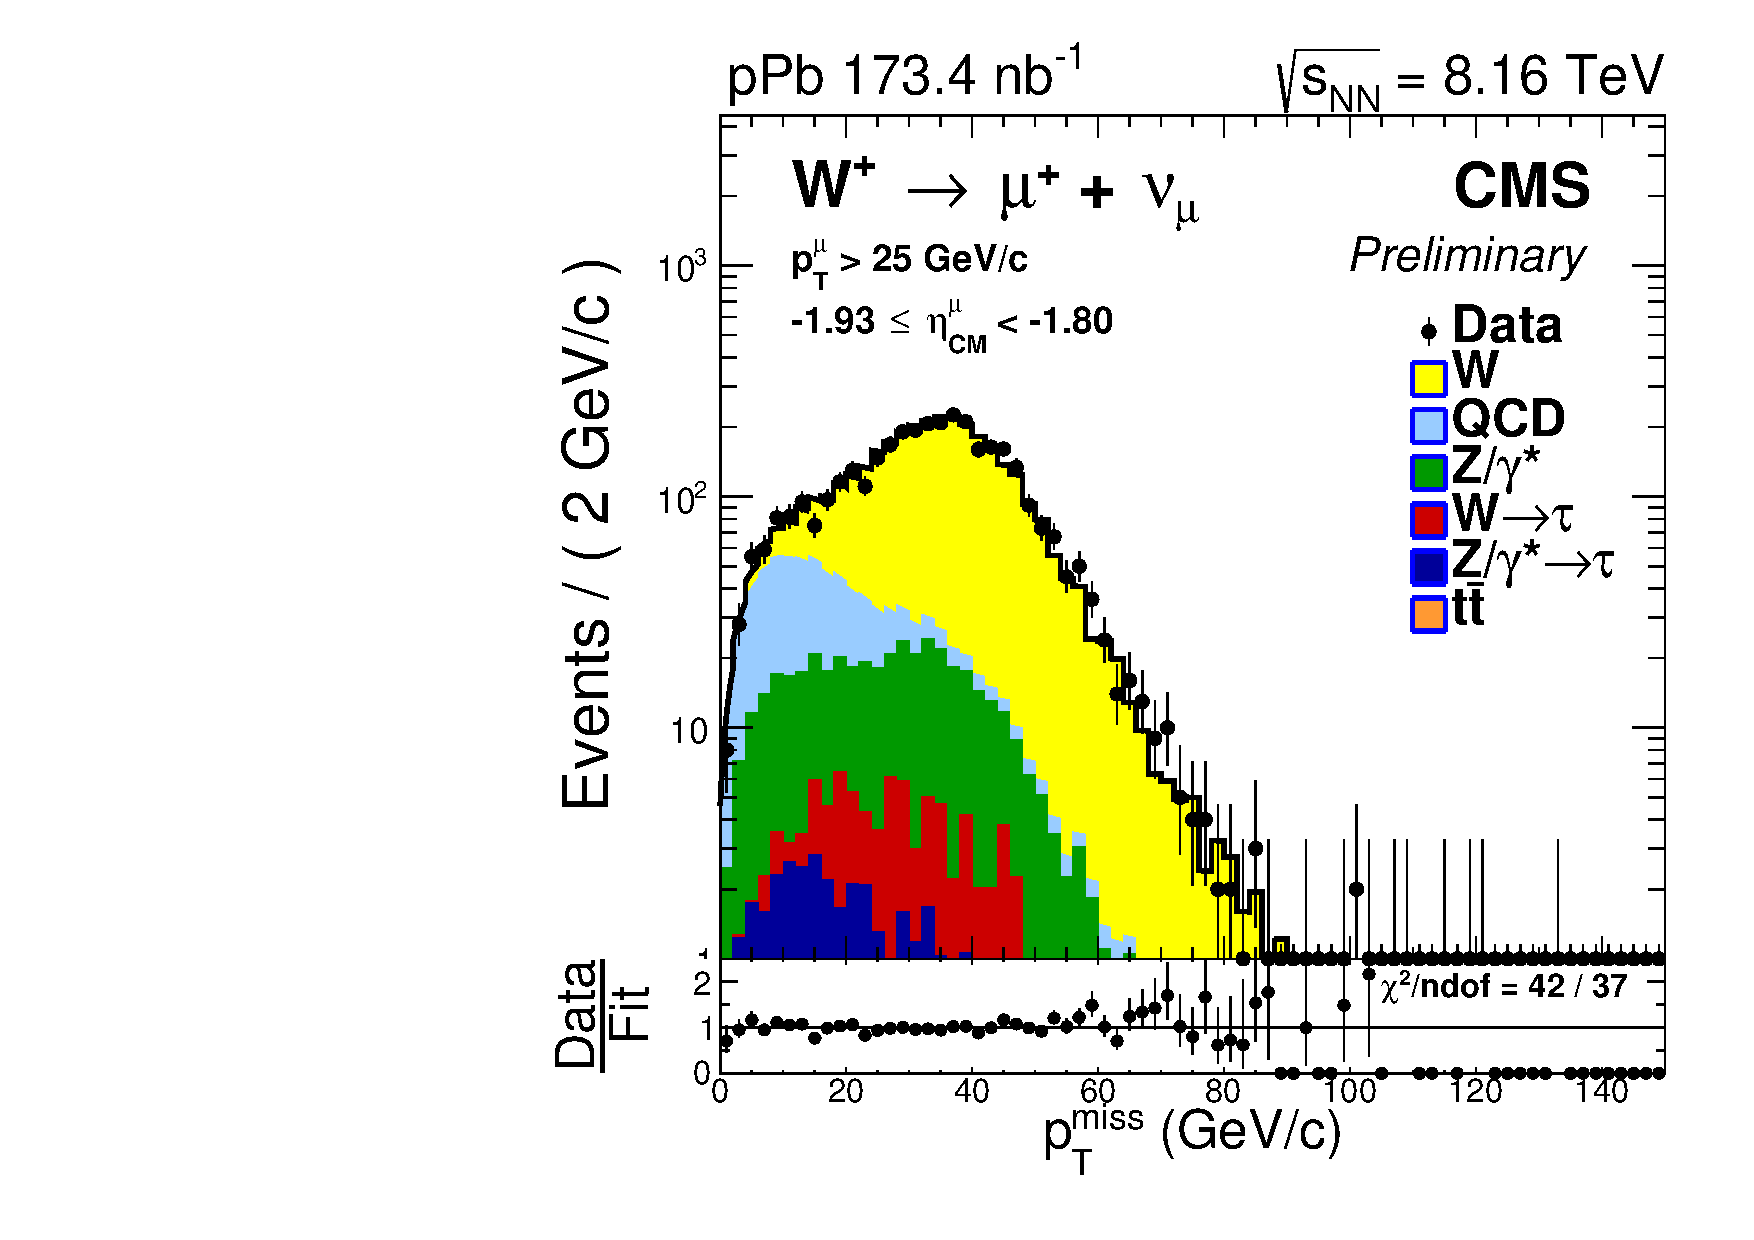
\includegraphics[width=0.23\textwidth]{Figures/WBoson/Analysis/SignalExtraction/Signal/LOG/PLOT_MET_DATA_WToMuPl_PA_Model_TEMP_WDYDYToTauWToTauTTbar_ModifiedRayleigh_QCD_MuEtaCM_-193_-180_MuIso_0_15.pdf}
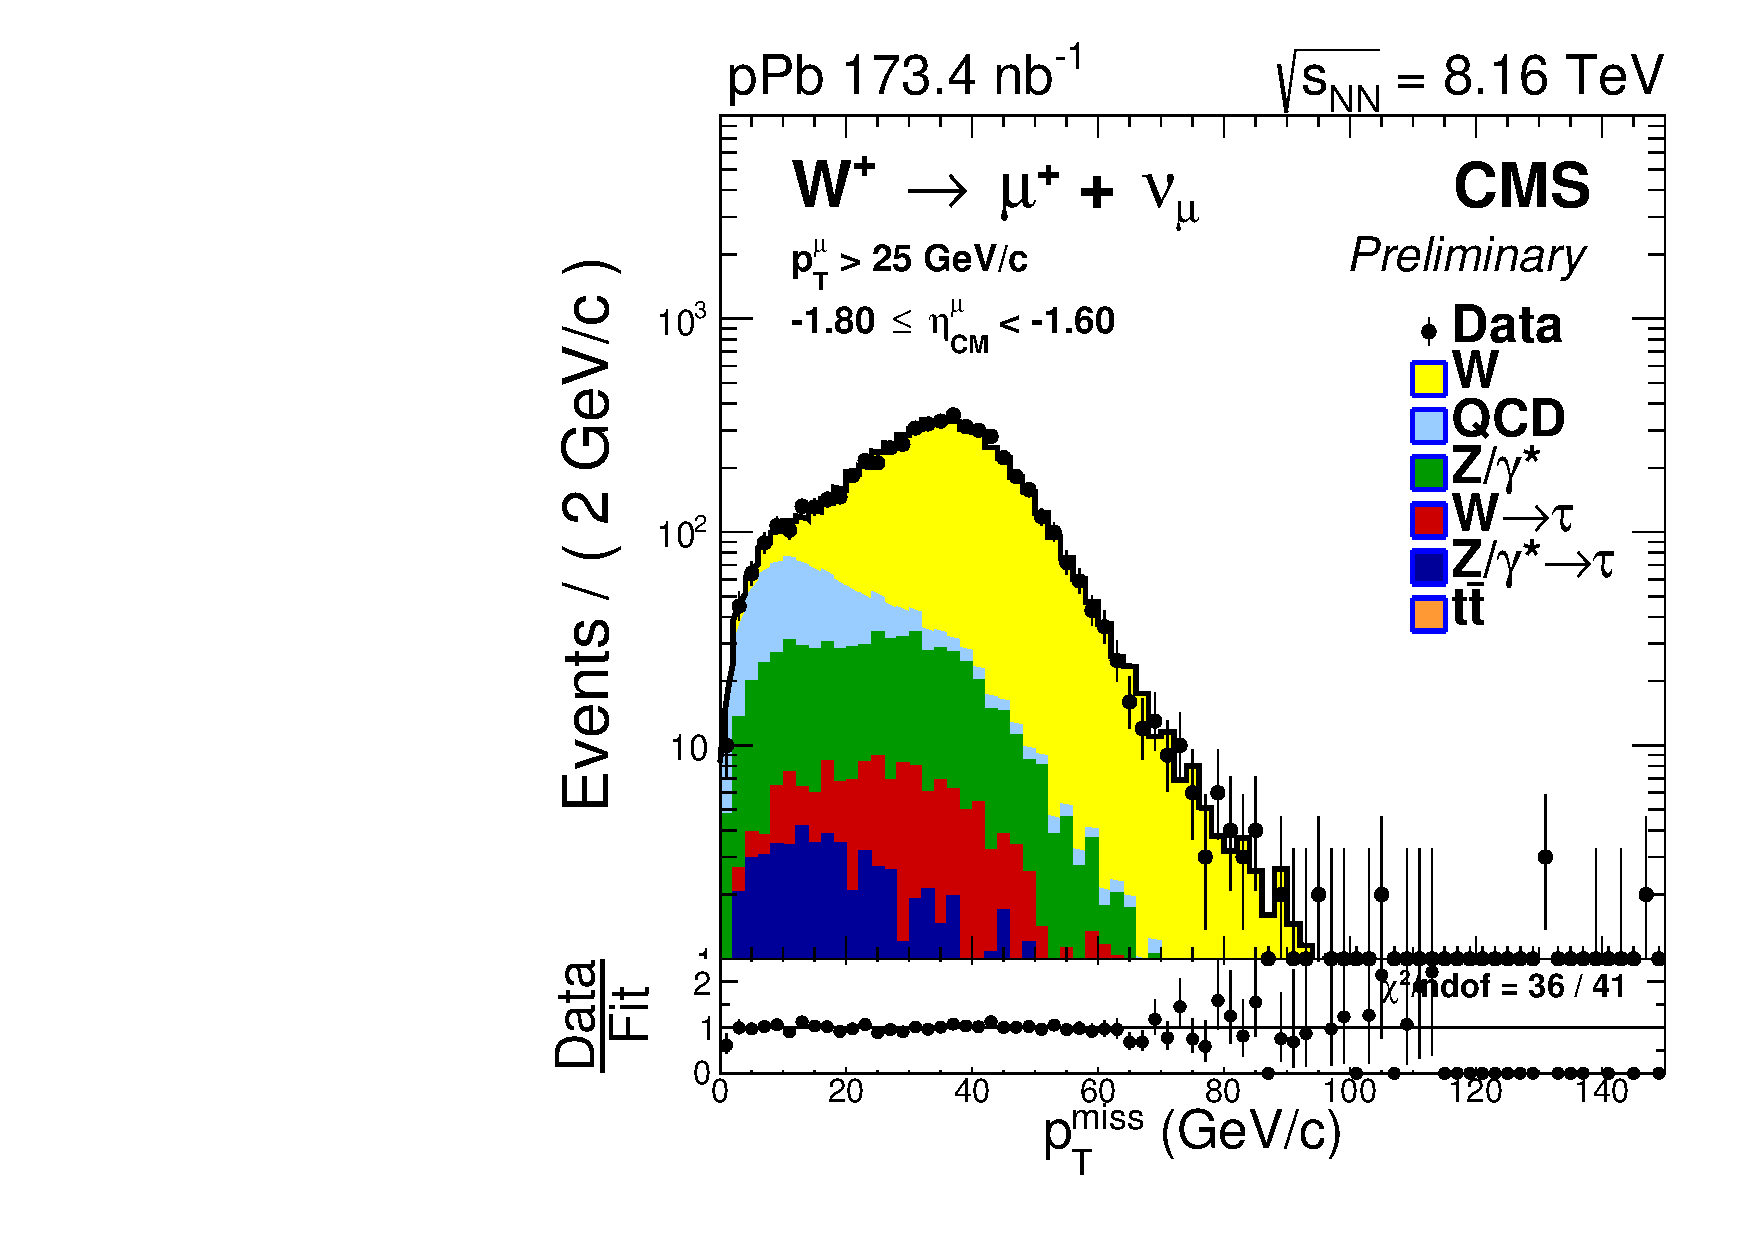
\includegraphics[width=0.23\textwidth]{Figures/WBoson/Analysis/SignalExtraction/Signal/LOG/PLOT_MET_DATA_WToMuPl_PA_Model_TEMP_WDYDYToTauWToTauTTbar_ModifiedRayleigh_QCD_MuEtaCM_-180_-160_MuIso_0_15.pdf}
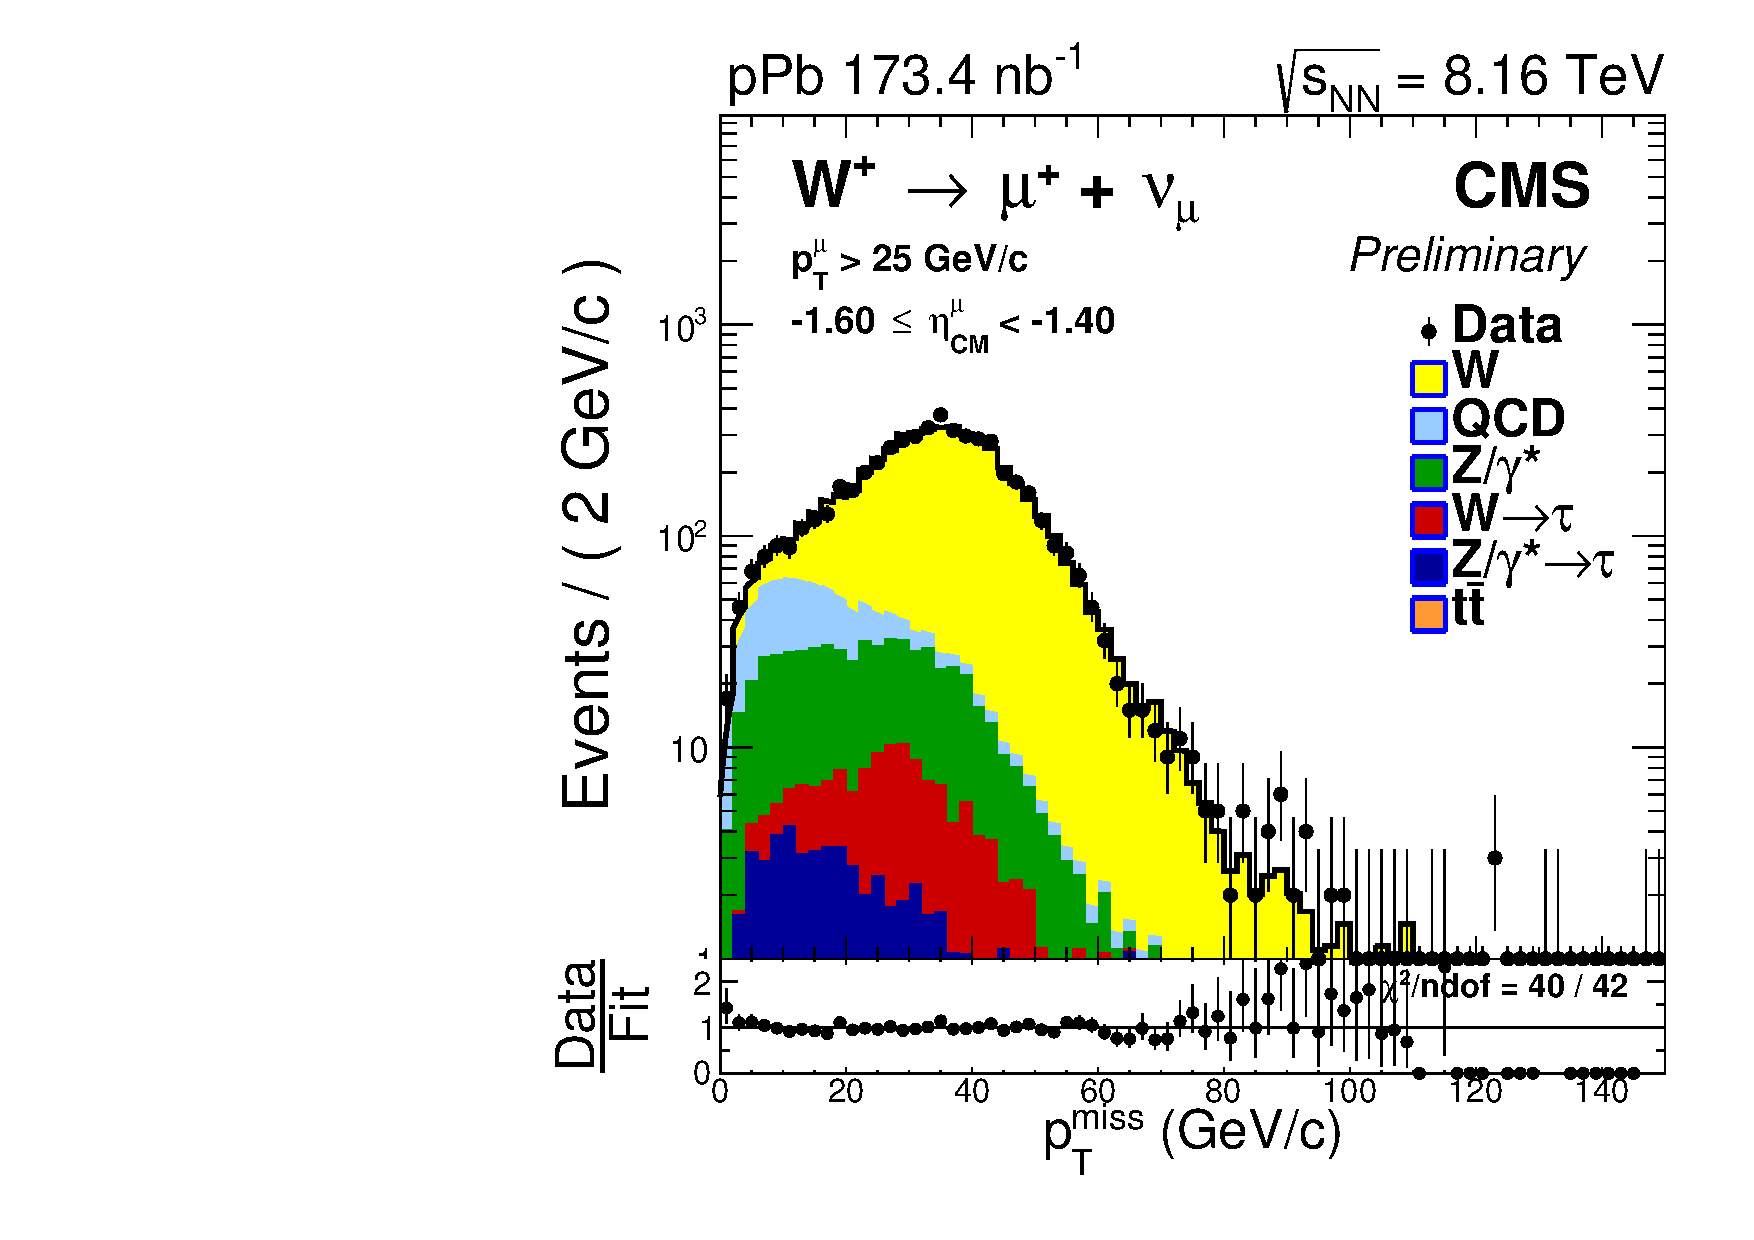
\includegraphics[width=0.23\textwidth]{Figures/WBoson/Analysis/SignalExtraction/Signal/LOG/PLOT_MET_DATA_WToMuPl_PA_Model_TEMP_WDYDYToTauWToTauTTbar_ModifiedRayleigh_QCD_MuEtaCM_-160_-140_MuIso_0_15.pdf}
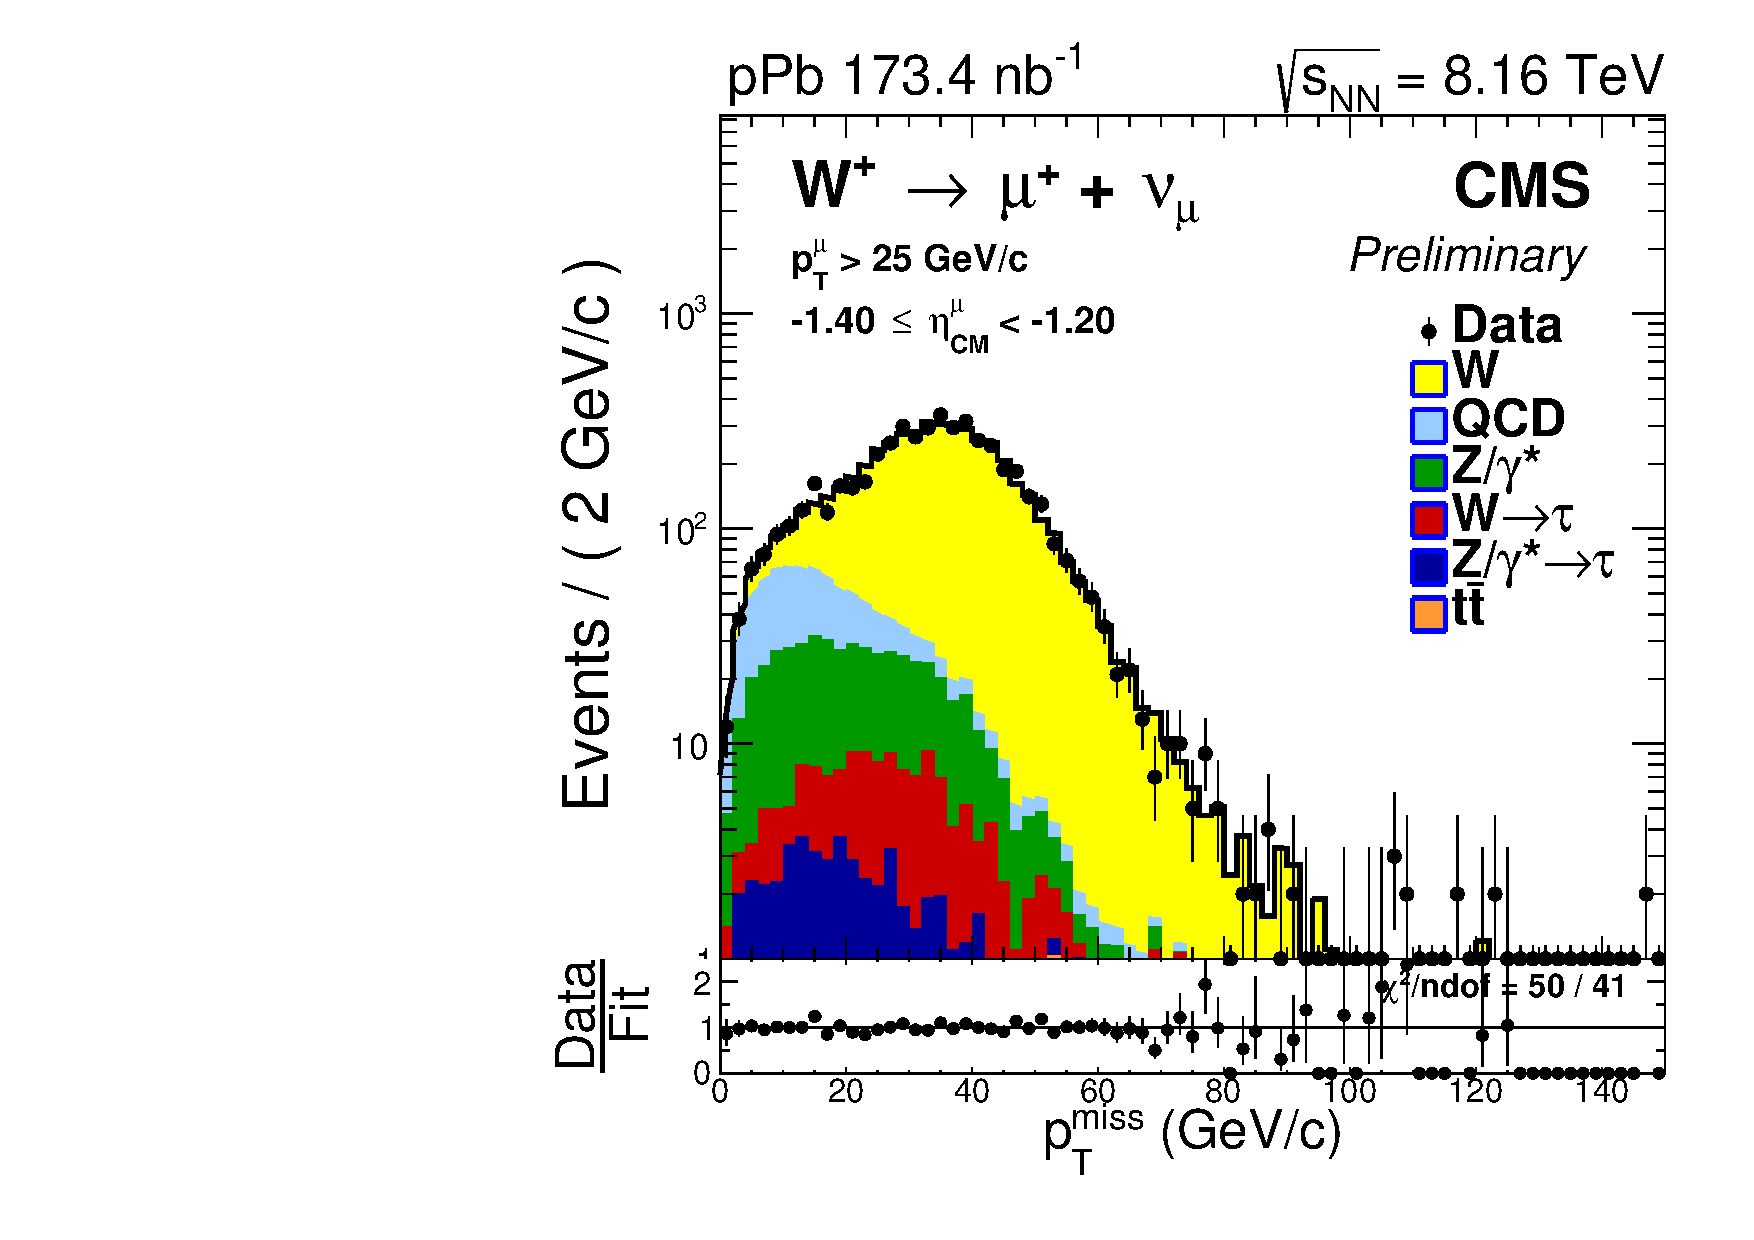
\includegraphics[width=0.23\textwidth]{Figures/WBoson/Analysis/SignalExtraction/Signal/LOG/PLOT_MET_DATA_WToMuPl_PA_Model_TEMP_WDYDYToTauWToTauTTbar_ModifiedRayleigh_QCD_MuEtaCM_-140_-120_MuIso_0_15.pdf}
\\
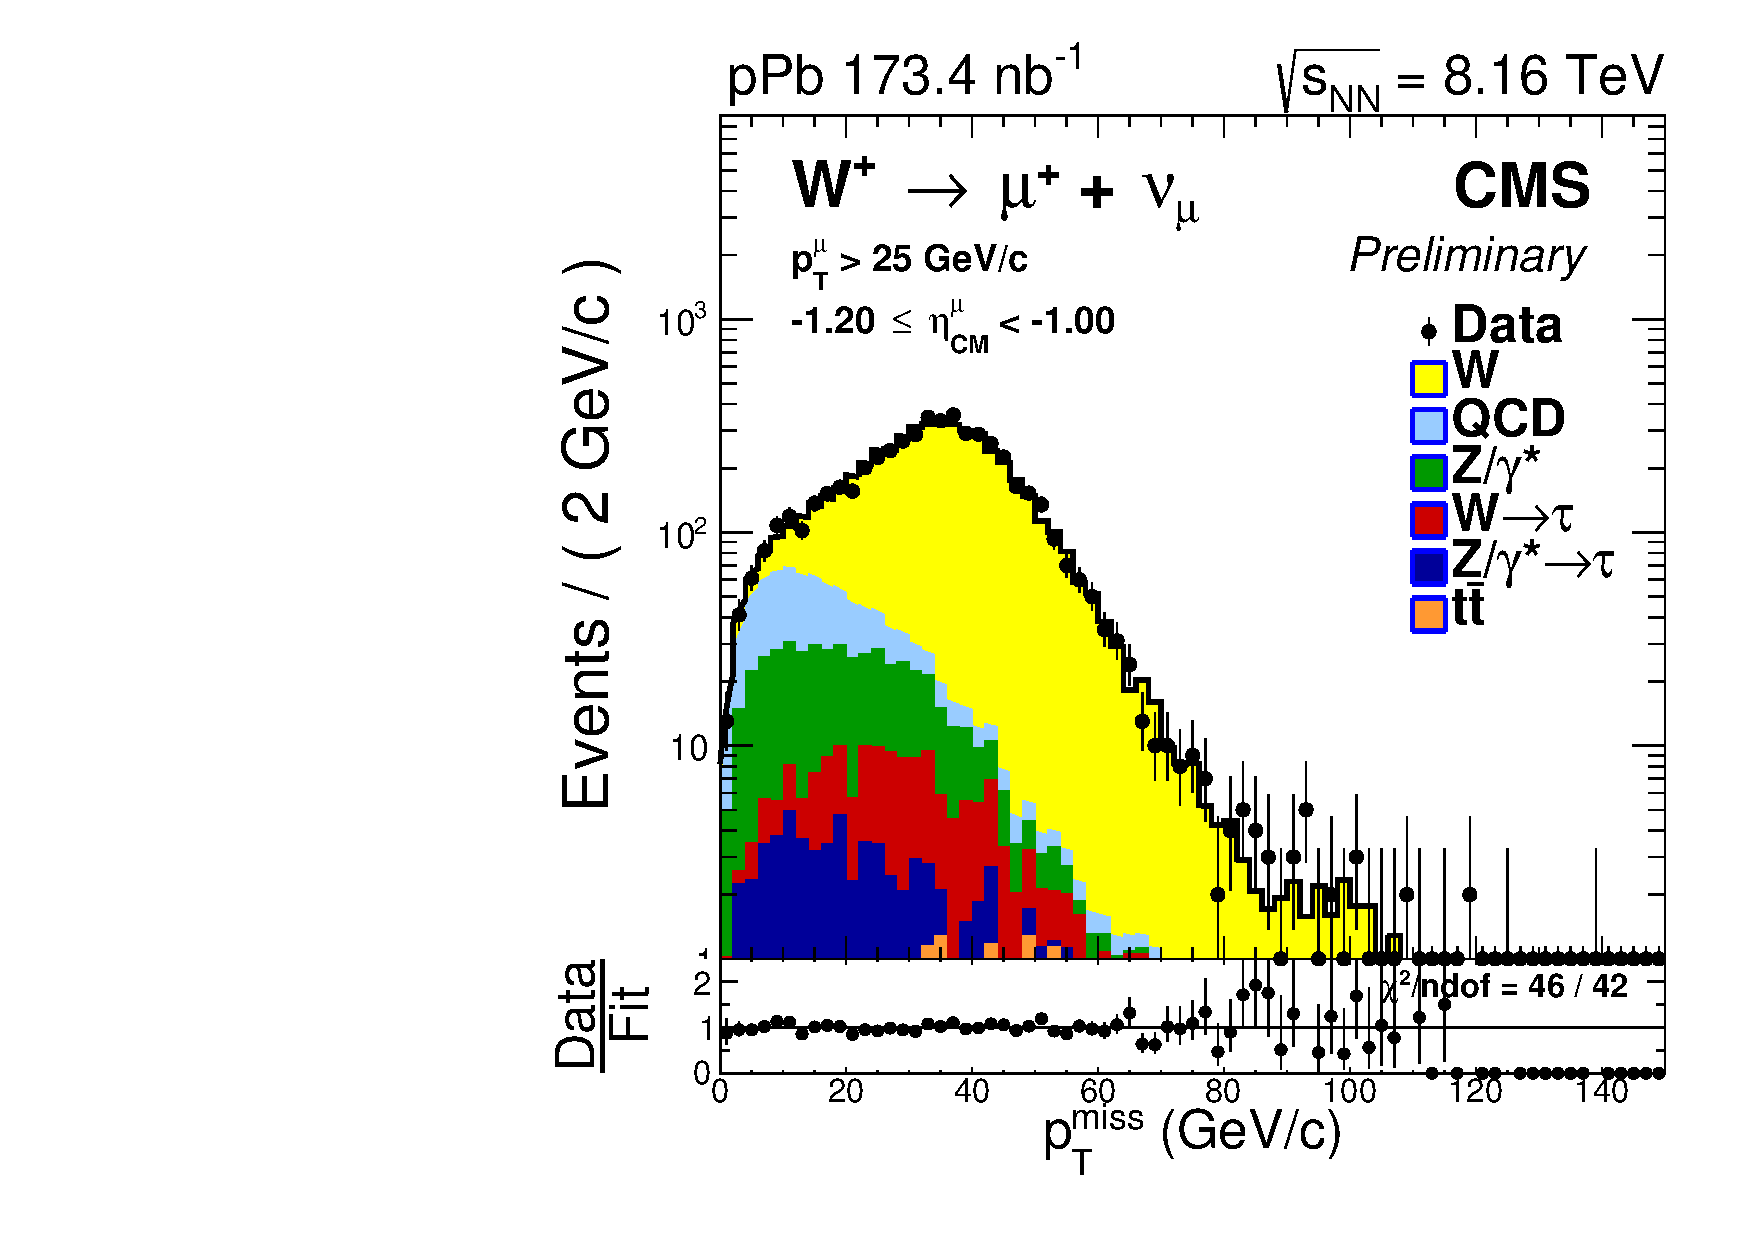
\includegraphics[width=0.23\textwidth]{Figures/WBoson/Analysis/SignalExtraction/Signal/LOG/PLOT_MET_DATA_WToMuPl_PA_Model_TEMP_WDYDYToTauWToTauTTbar_ModifiedRayleigh_QCD_MuEtaCM_-120_-100_MuIso_0_15.pdf}
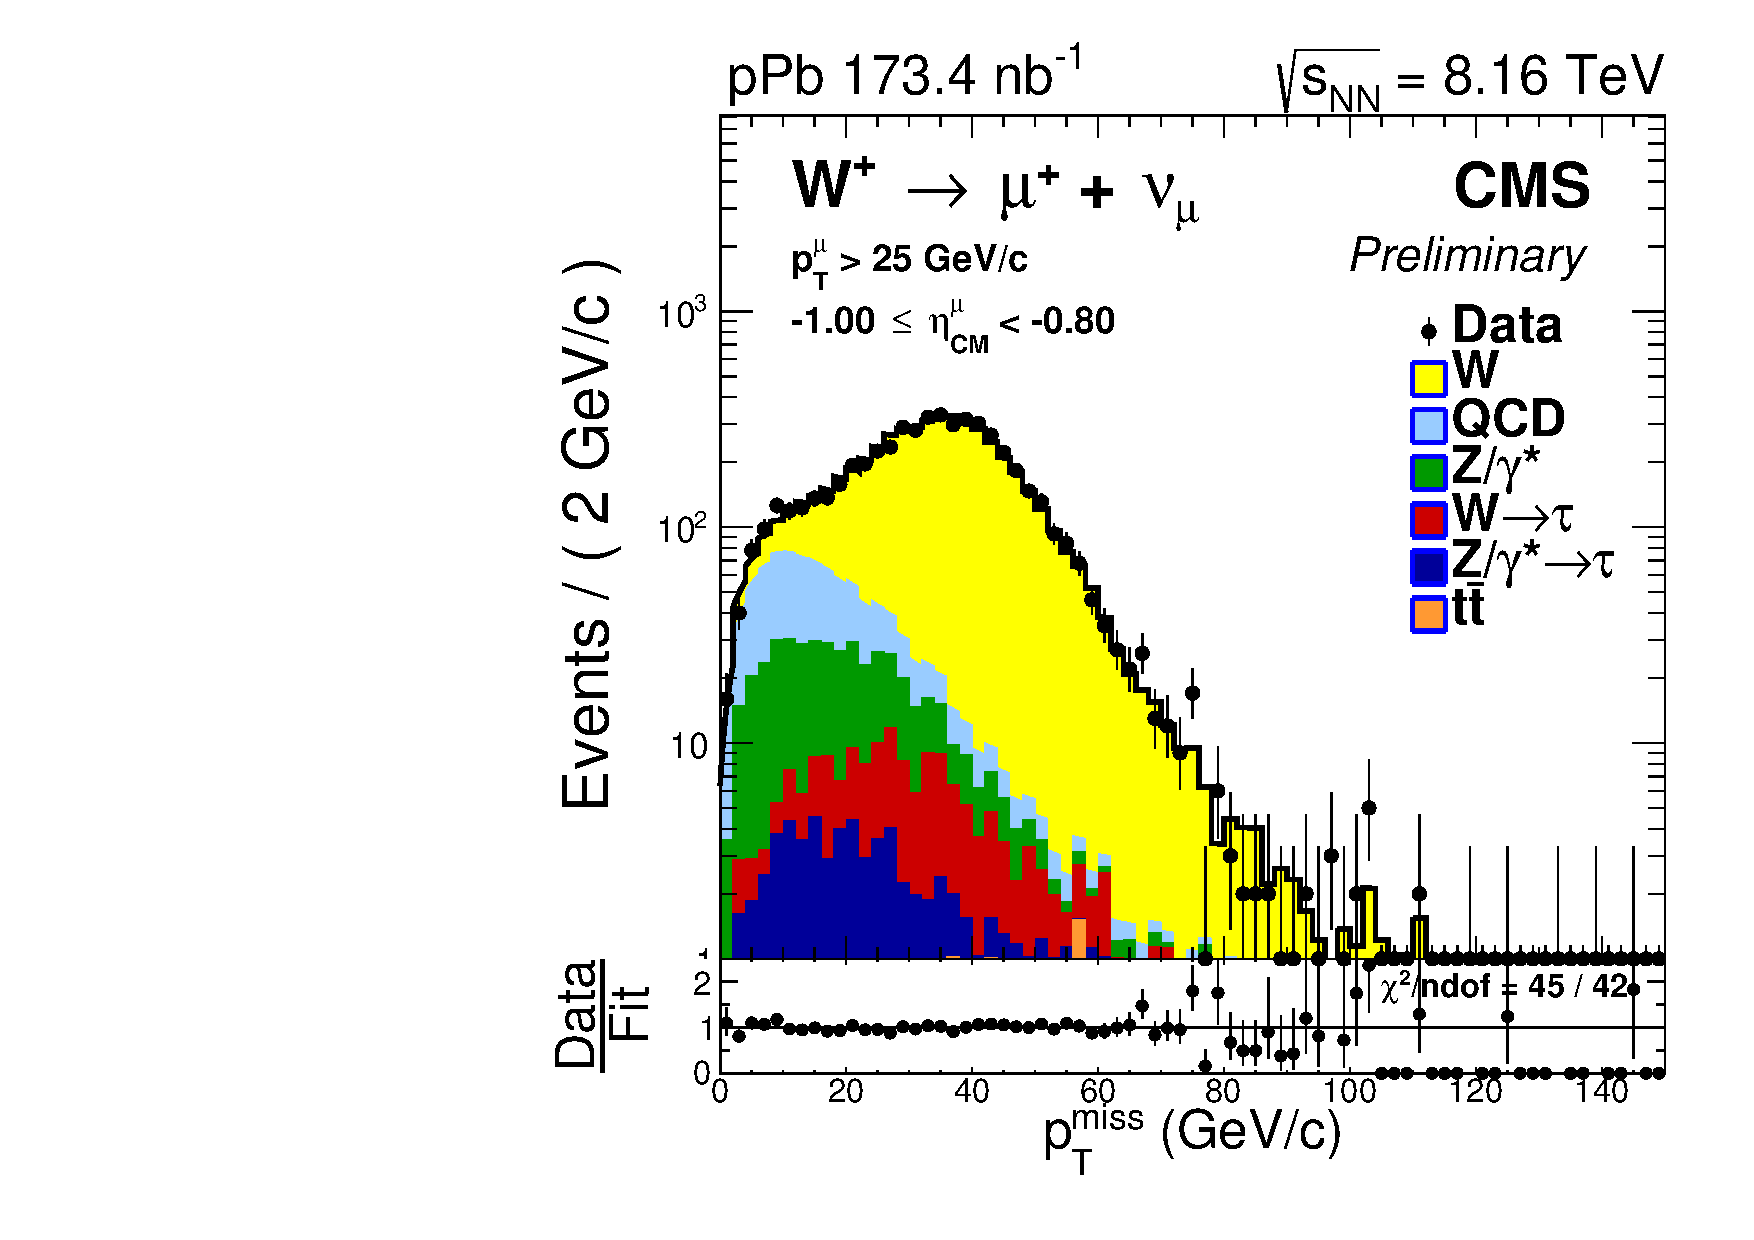
\includegraphics[width=0.23\textwidth]{Figures/WBoson/Analysis/SignalExtraction/Signal/LOG/PLOT_MET_DATA_WToMuPl_PA_Model_TEMP_WDYDYToTauWToTauTTbar_ModifiedRayleigh_QCD_MuEtaCM_-100_-80_MuIso_0_15.pdf}
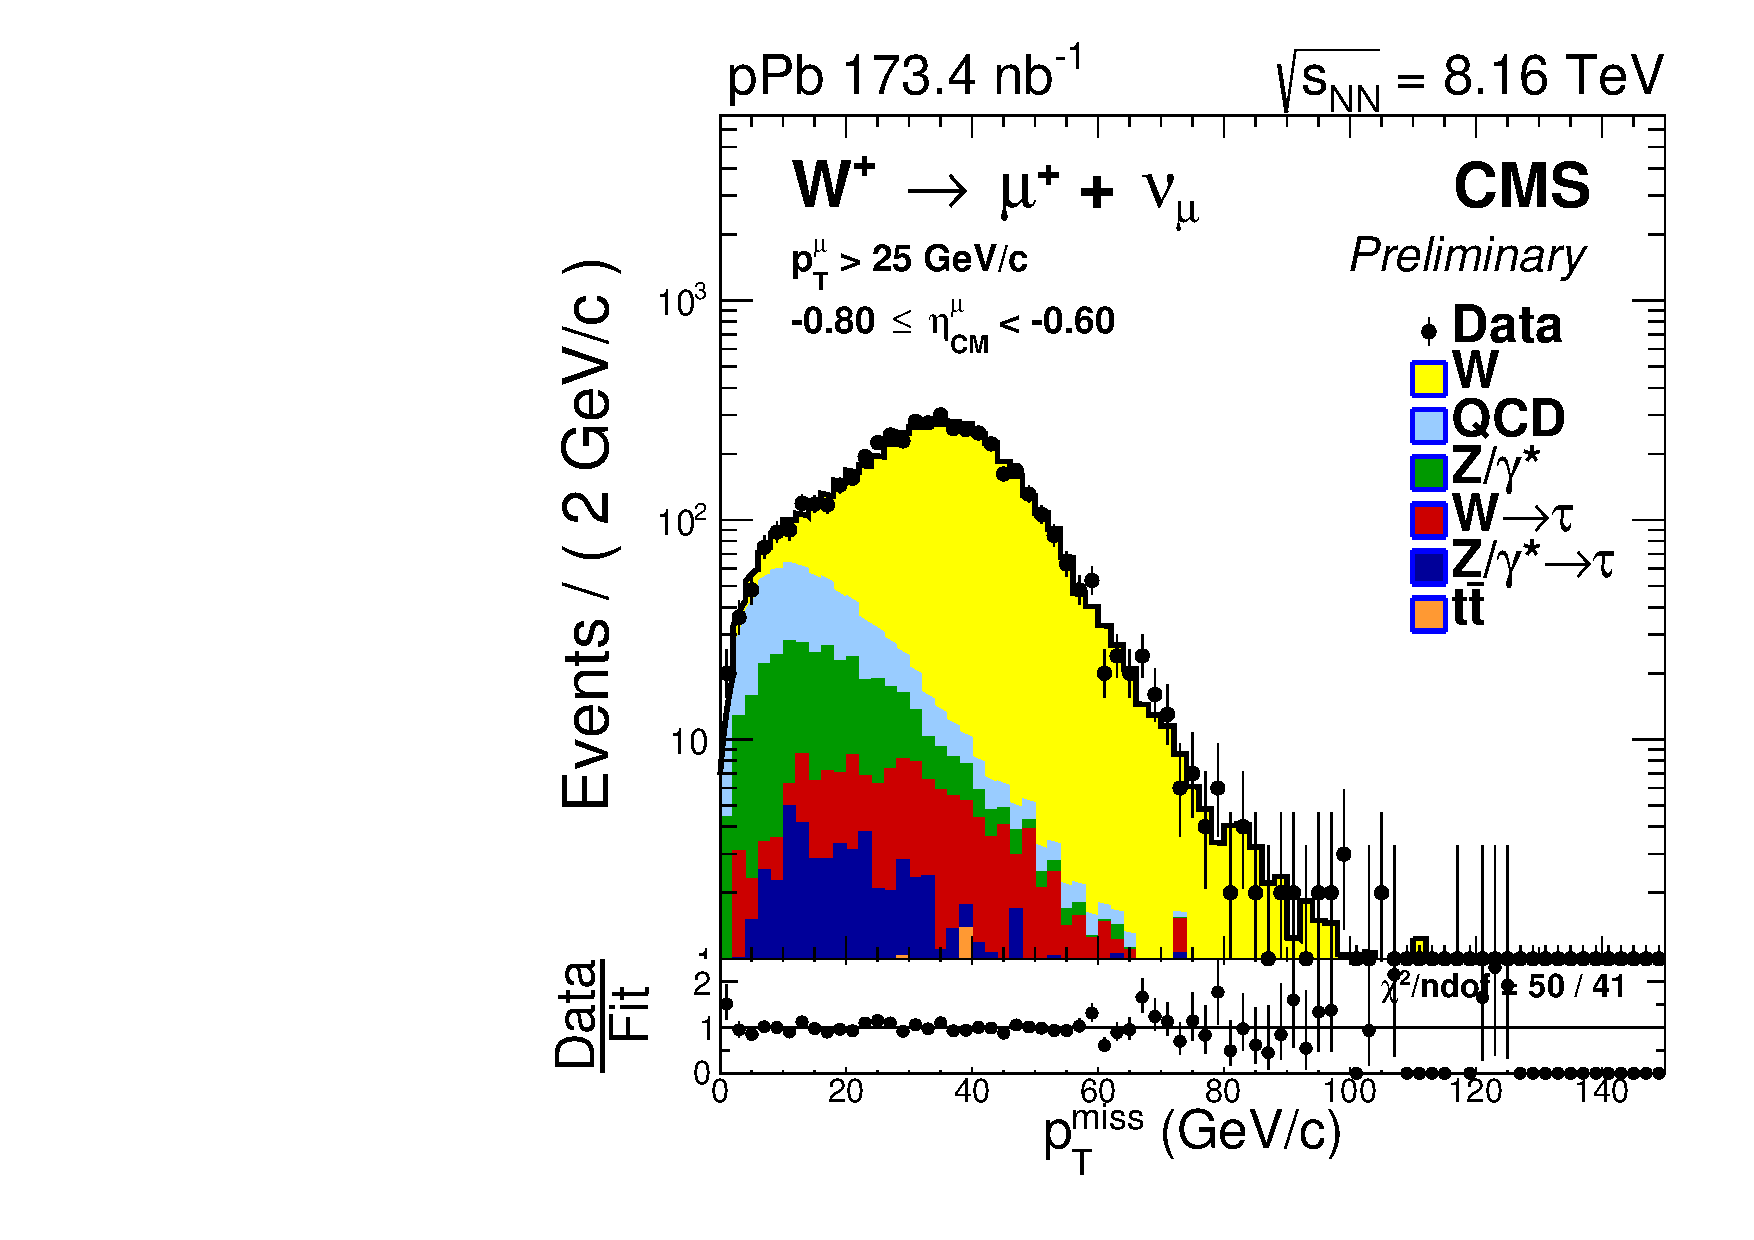
\includegraphics[width=0.23\textwidth]{Figures/WBoson/Analysis/SignalExtraction/Signal/LOG/PLOT_MET_DATA_WToMuPl_PA_Model_TEMP_WDYDYToTauWToTauTTbar_ModifiedRayleigh_QCD_MuEtaCM_-80_-60_MuIso_0_15.pdf}
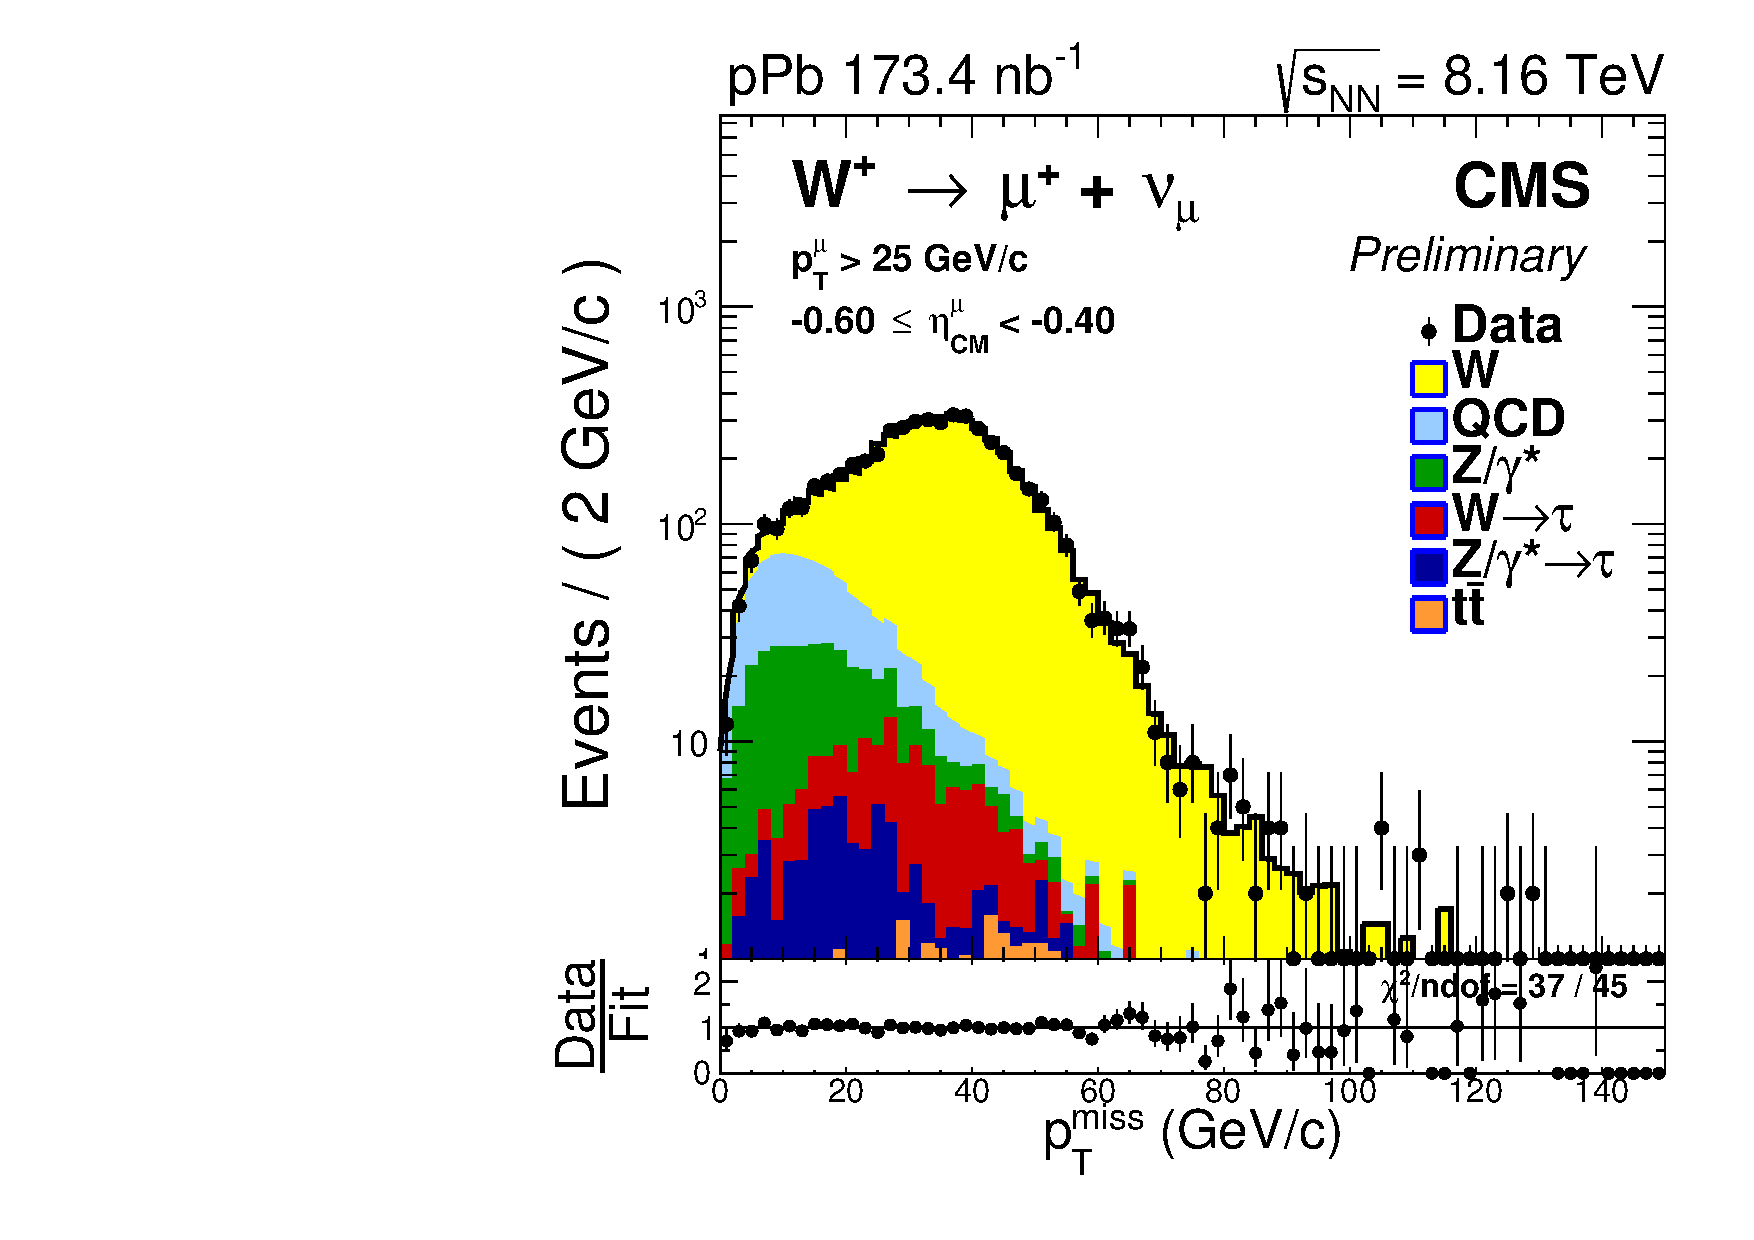
\includegraphics[width=0.23\textwidth]{Figures/WBoson/Analysis/SignalExtraction/Signal/LOG/PLOT_MET_DATA_WToMuPl_PA_Model_TEMP_WDYDYToTauWToTauTTbar_ModifiedRayleigh_QCD_MuEtaCM_-60_-40_MuIso_0_15.pdf}
\\
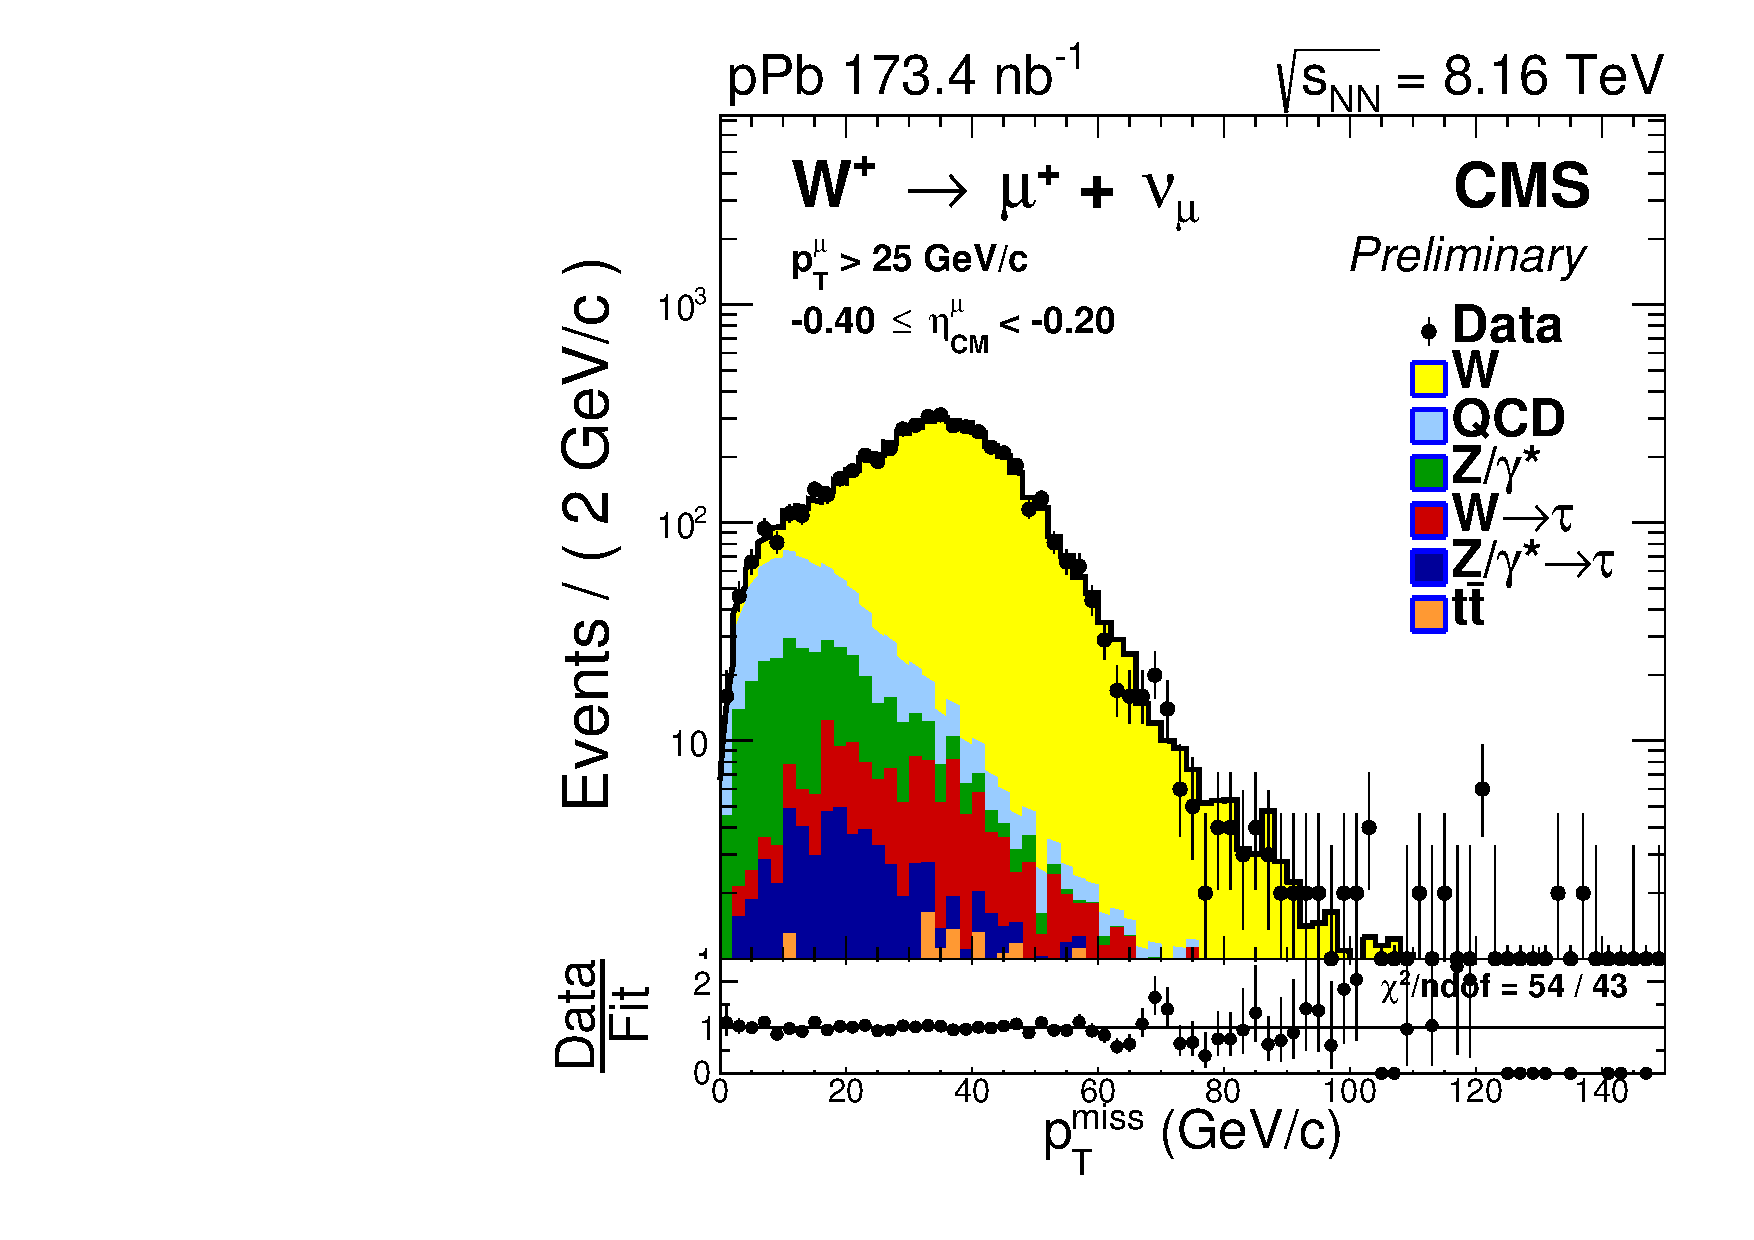
\includegraphics[width=0.23\textwidth]{Figures/WBoson/Analysis/SignalExtraction/Signal/LOG/PLOT_MET_DATA_WToMuPl_PA_Model_TEMP_WDYDYToTauWToTauTTbar_ModifiedRayleigh_QCD_MuEtaCM_-40_-20_MuIso_0_15.pdf}
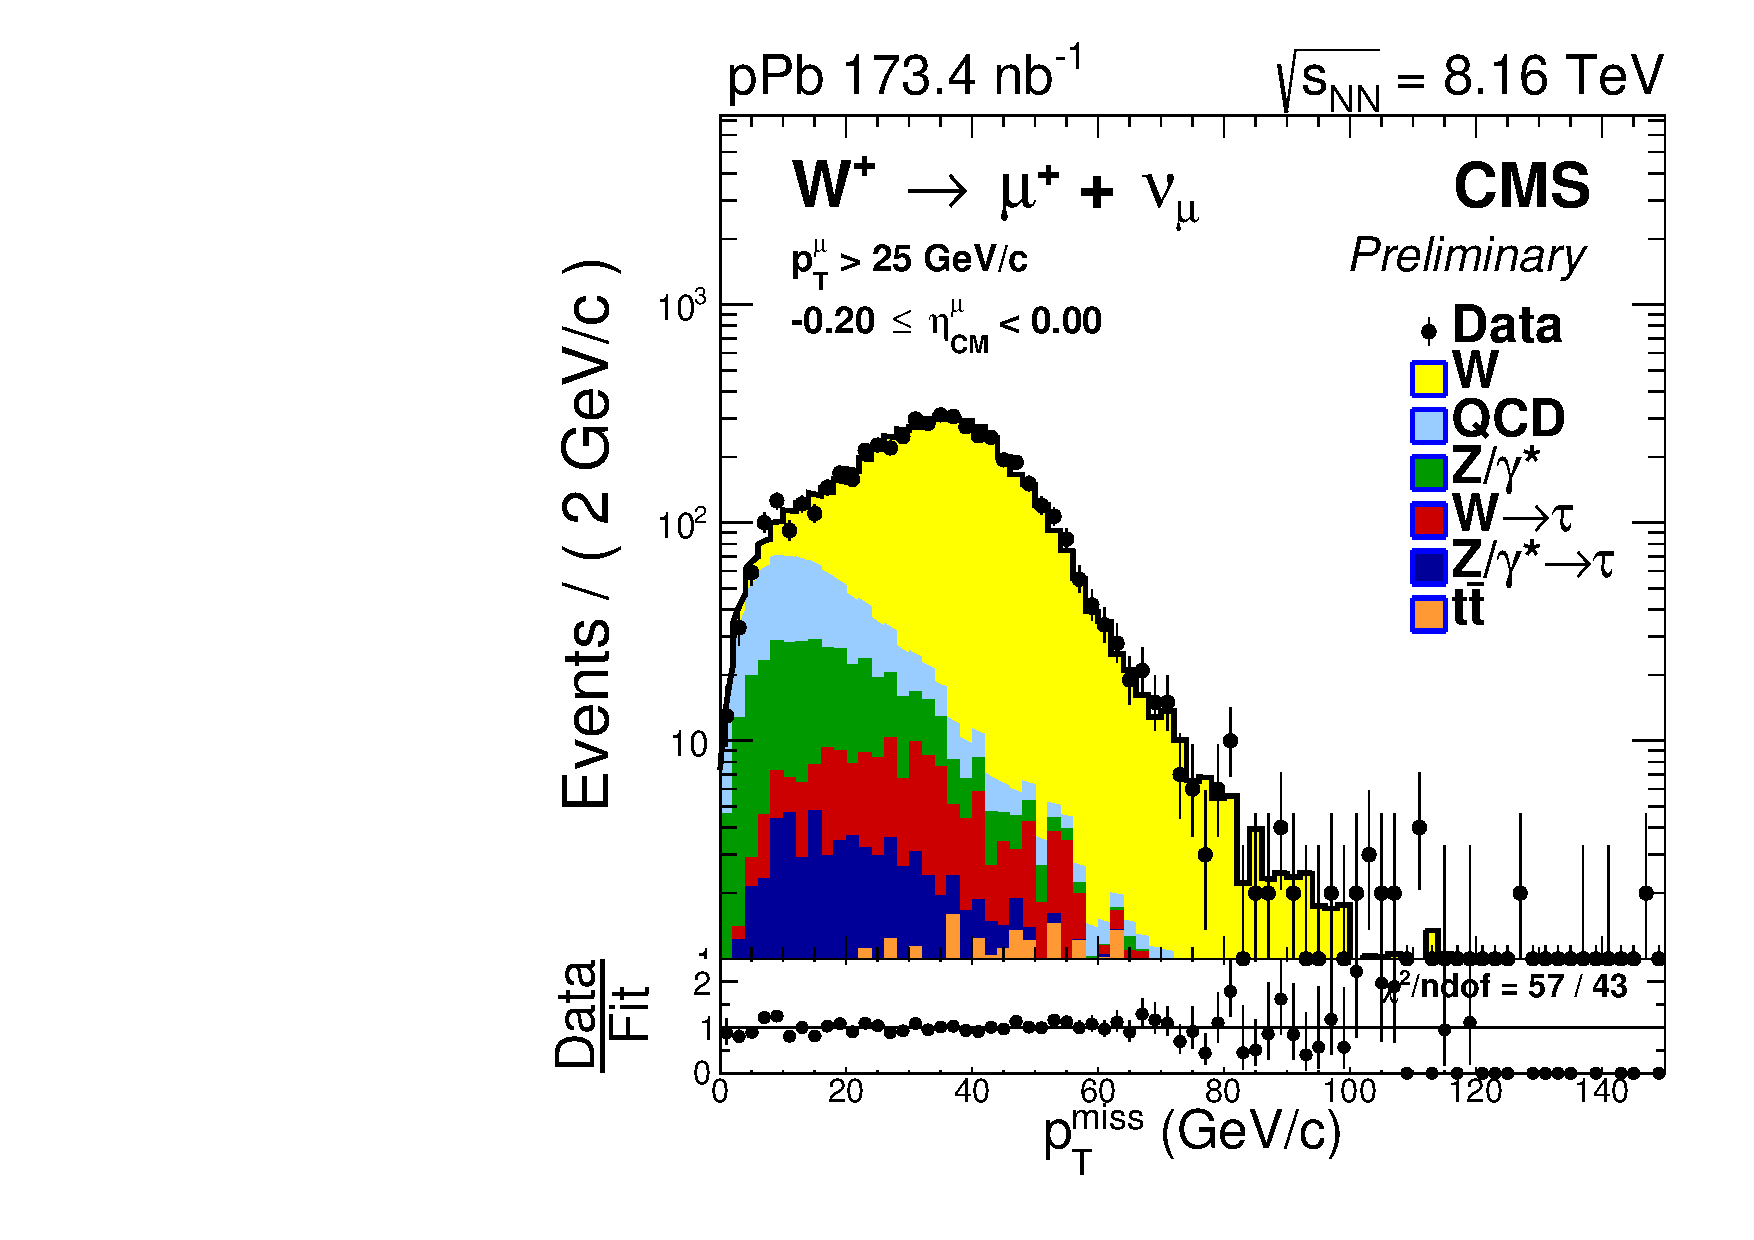
\includegraphics[width=0.23\textwidth]{Figures/WBoson/Analysis/SignalExtraction/Signal/LOG/PLOT_MET_DATA_WToMuPl_PA_Model_TEMP_WDYDYToTauWToTauTTbar_ModifiedRayleigh_QCD_MuEtaCM_-20_0_MuIso_0_15.pdf}
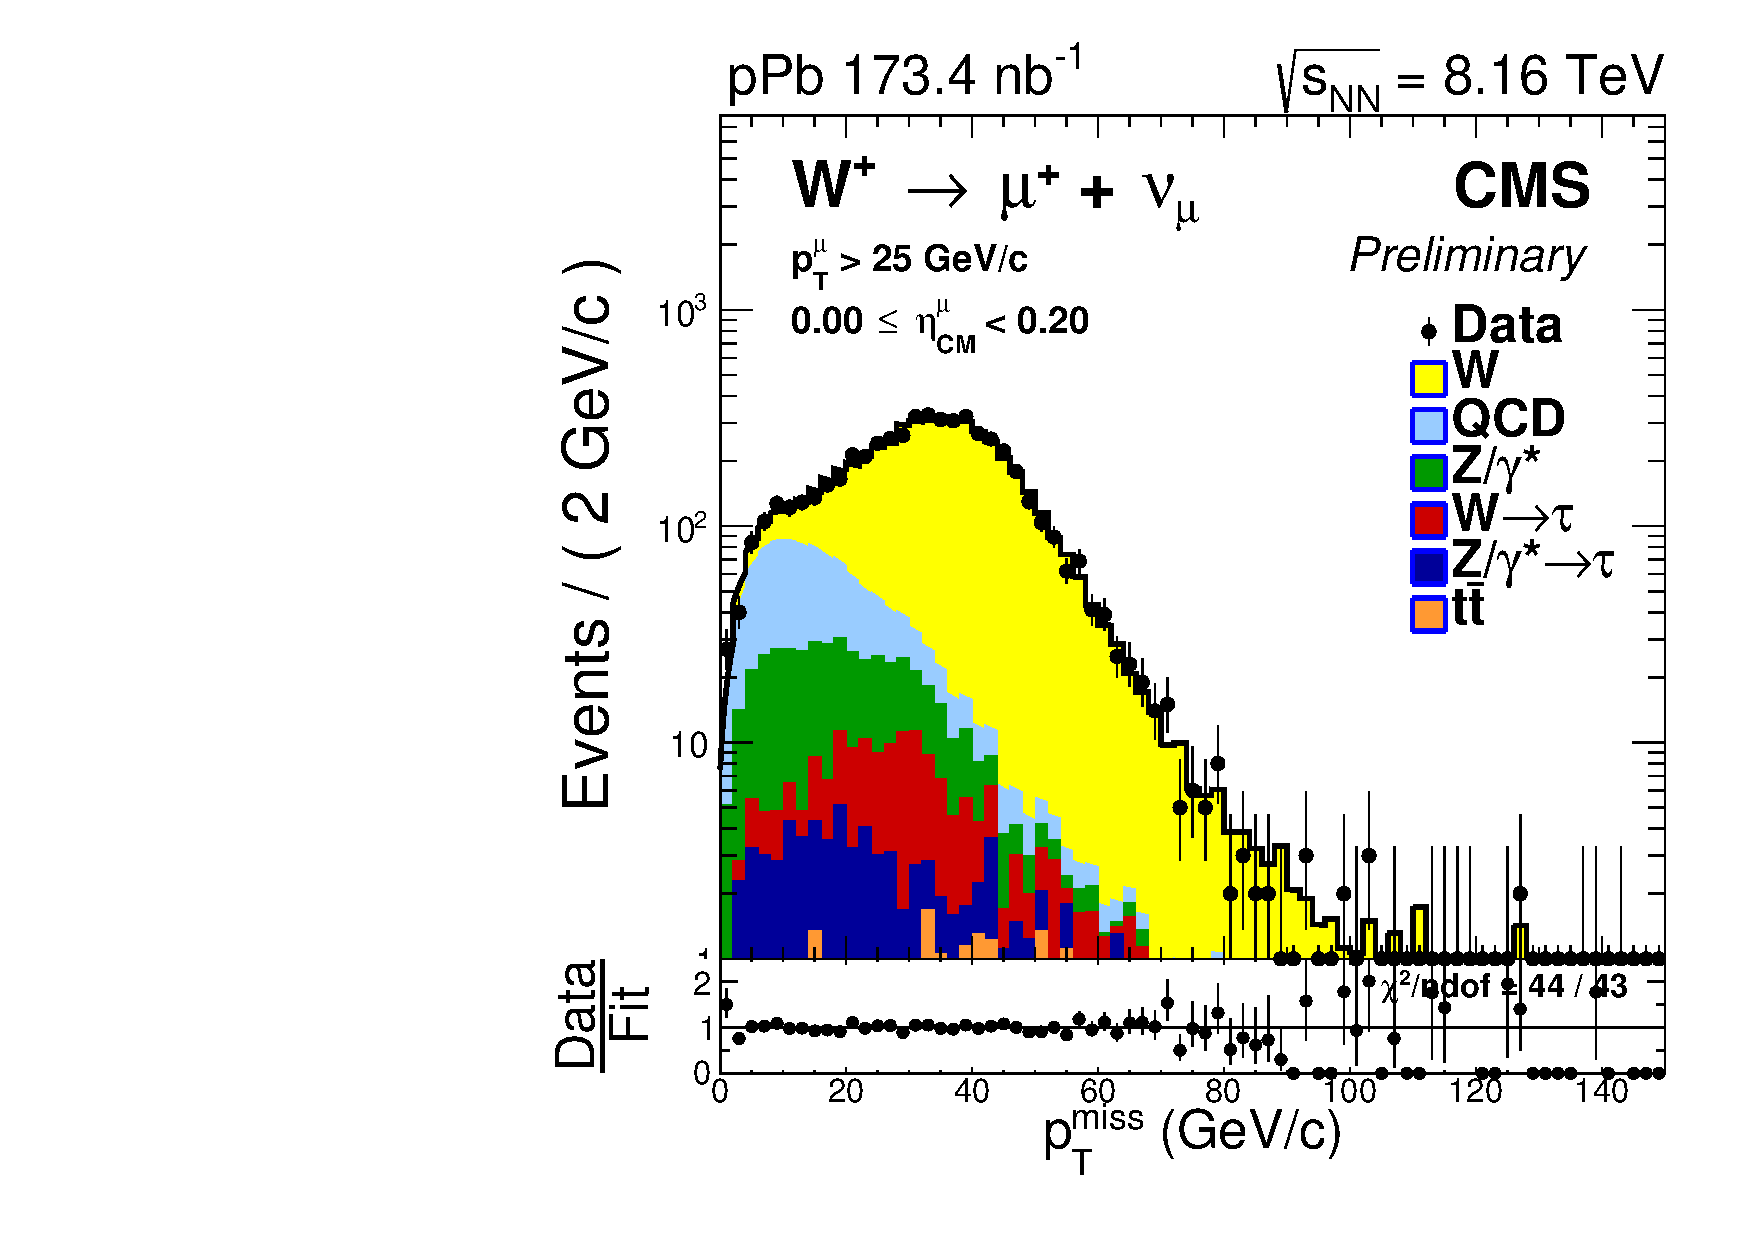
\includegraphics[width=0.23\textwidth]{Figures/WBoson/Analysis/SignalExtraction/Signal/LOG/PLOT_MET_DATA_WToMuPl_PA_Model_TEMP_WDYDYToTauWToTauTTbar_ModifiedRayleigh_QCD_MuEtaCM_0_20_MuIso_0_15.pdf}
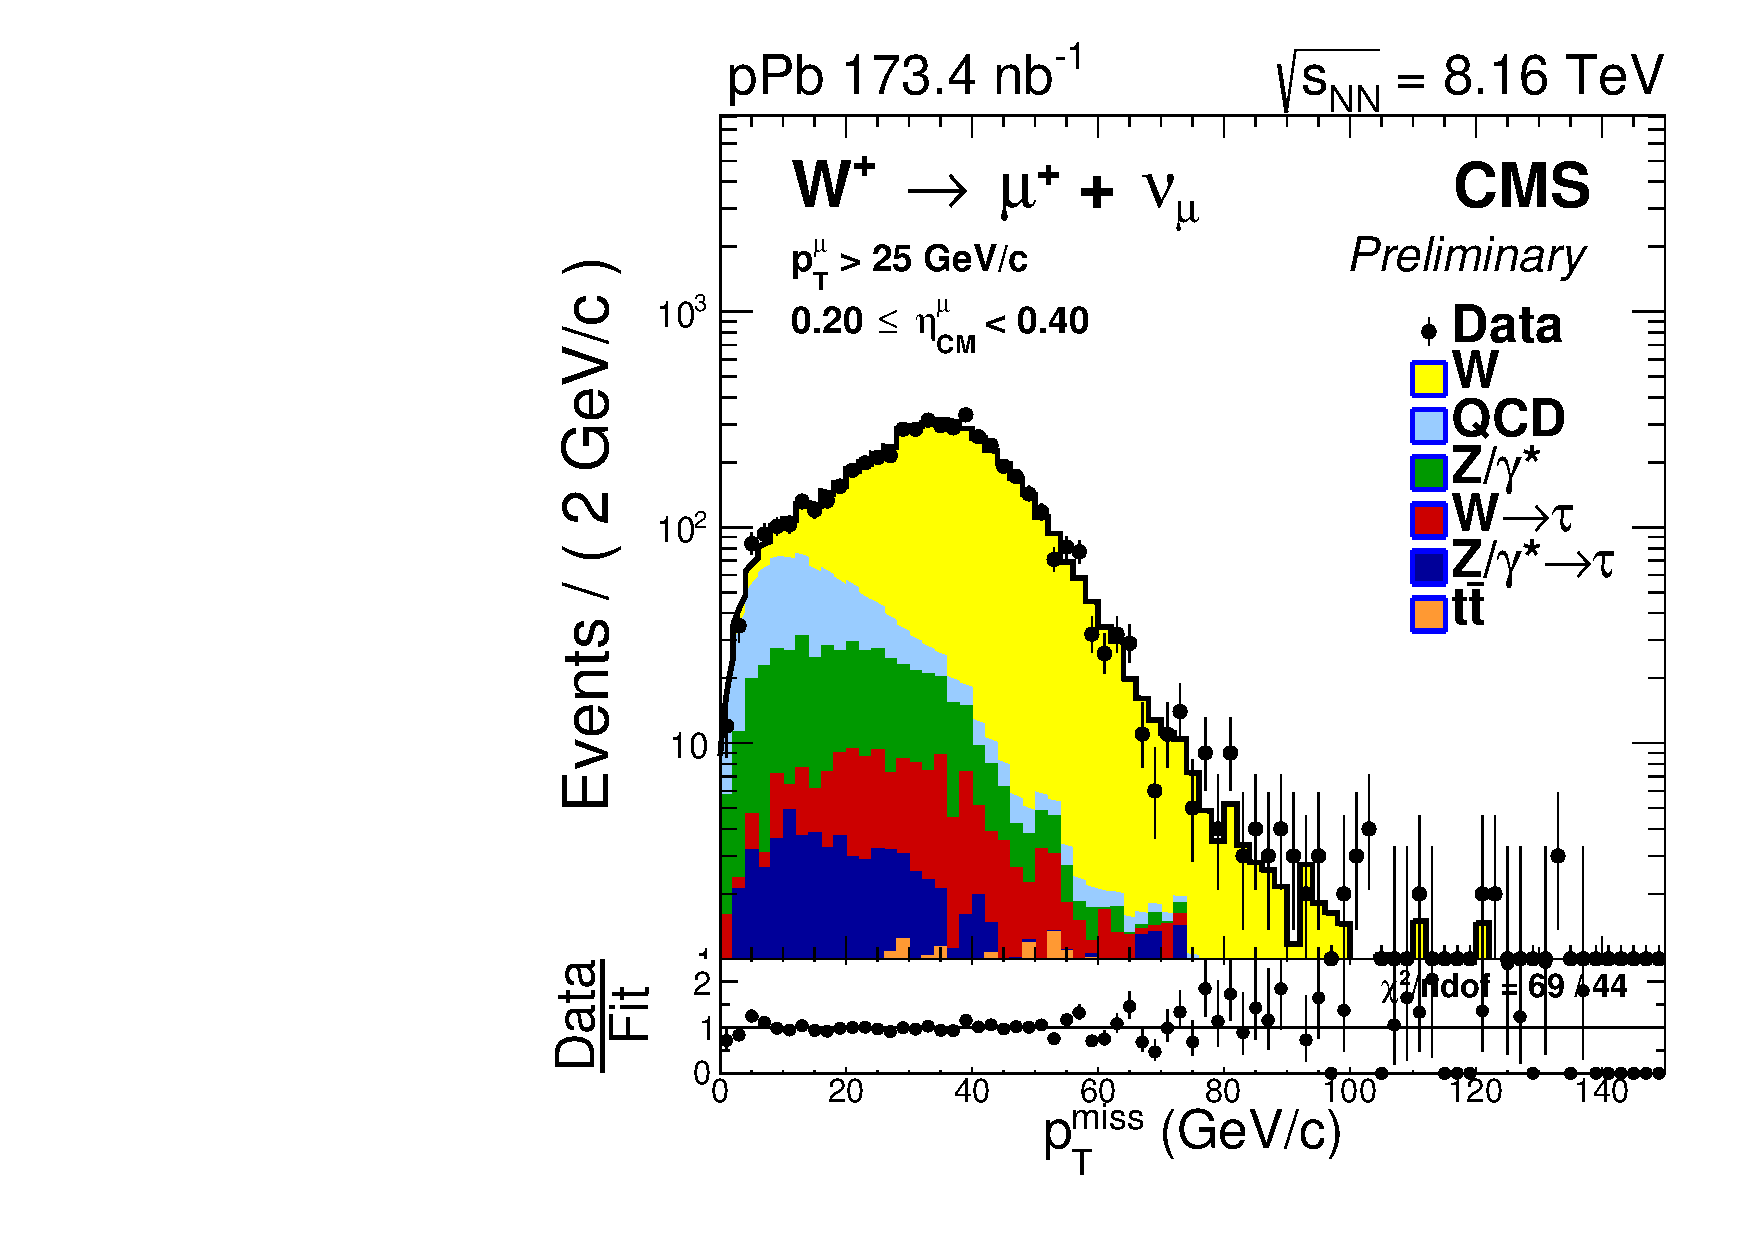
\includegraphics[width=0.23\textwidth]{Figures/WBoson/Analysis/SignalExtraction/Signal/LOG/PLOT_MET_DATA_WToMuPl_PA_Model_TEMP_WDYDYToTauWToTauTTbar_ModifiedRayleigh_QCD_MuEtaCM_20_40_MuIso_0_15.pdf}
\\
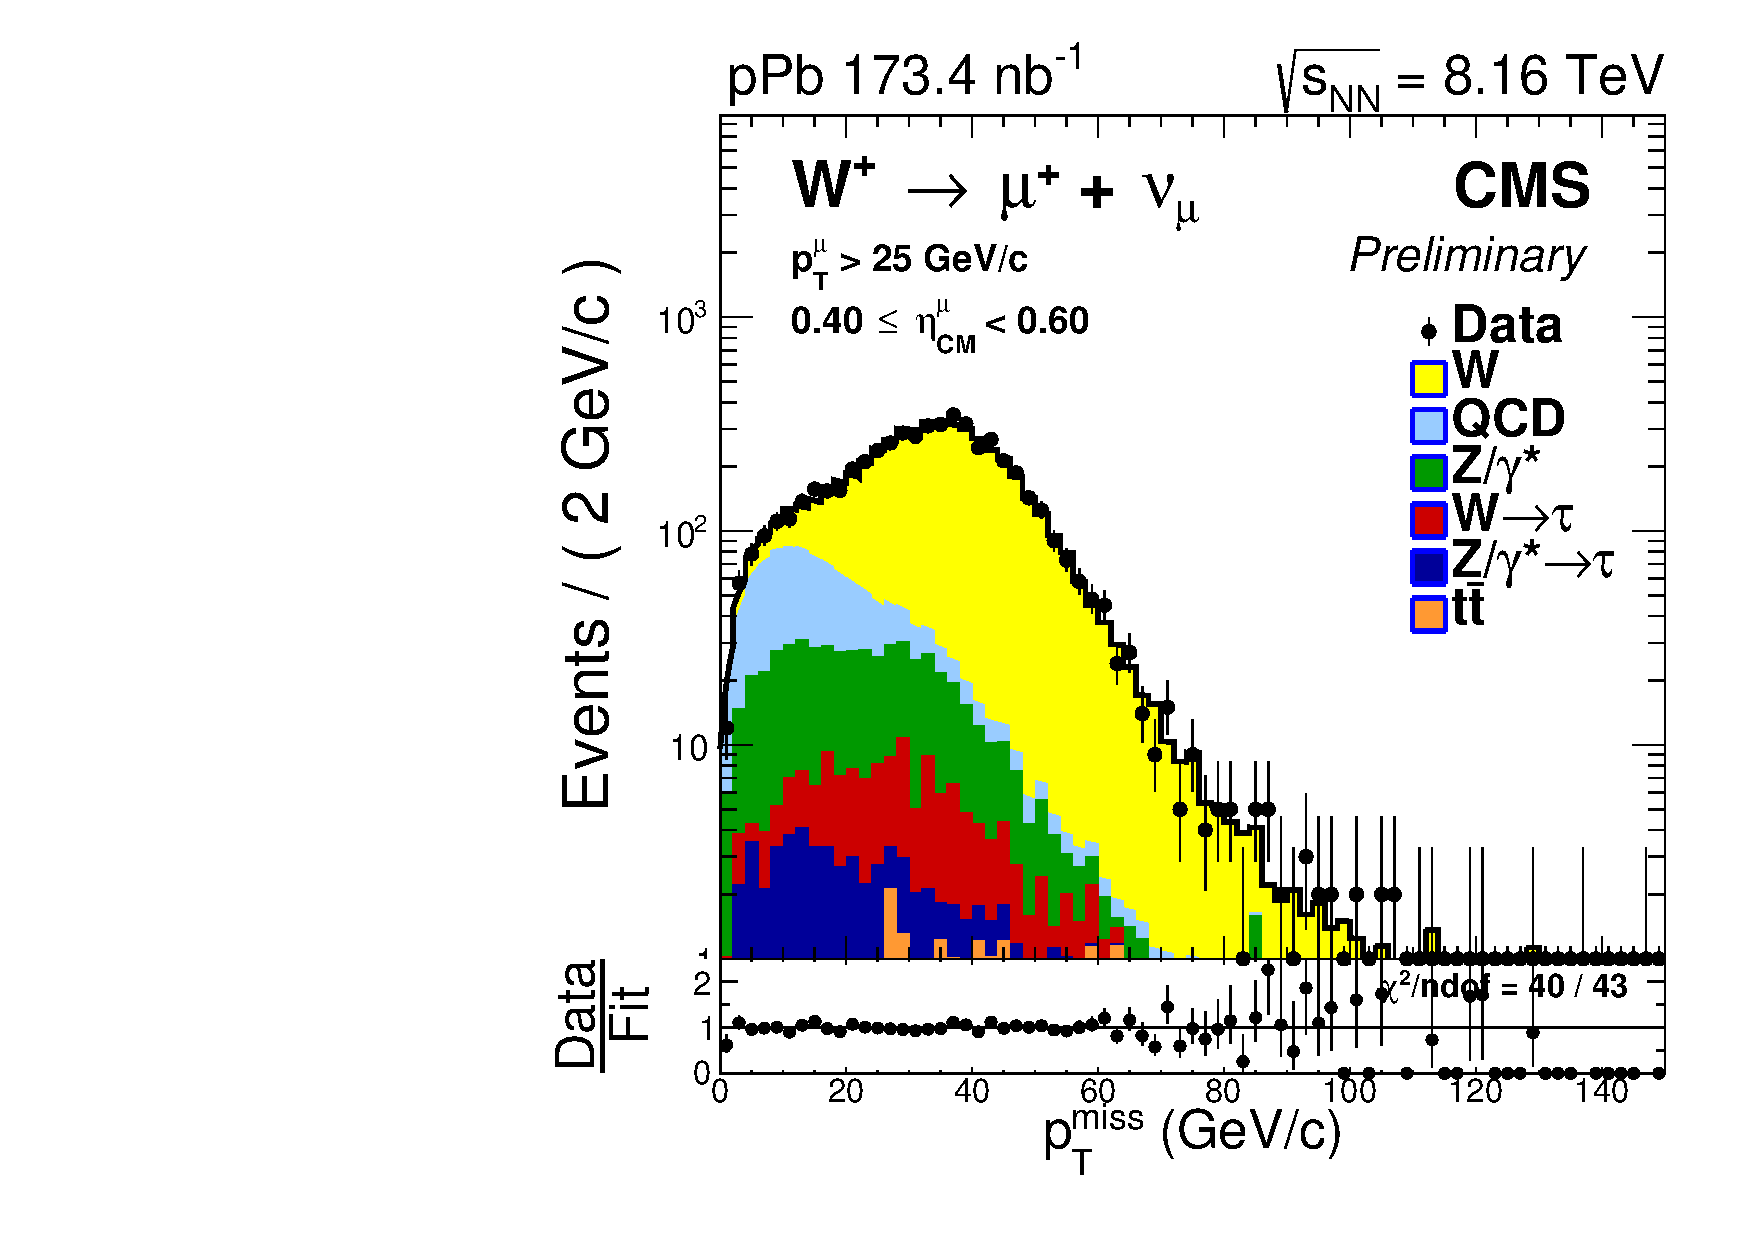
\includegraphics[width=0.23\textwidth]{Figures/WBoson/Analysis/SignalExtraction/Signal/LOG/PLOT_MET_DATA_WToMuPl_PA_Model_TEMP_WDYDYToTauWToTauTTbar_ModifiedRayleigh_QCD_MuEtaCM_40_60_MuIso_0_15.pdf}
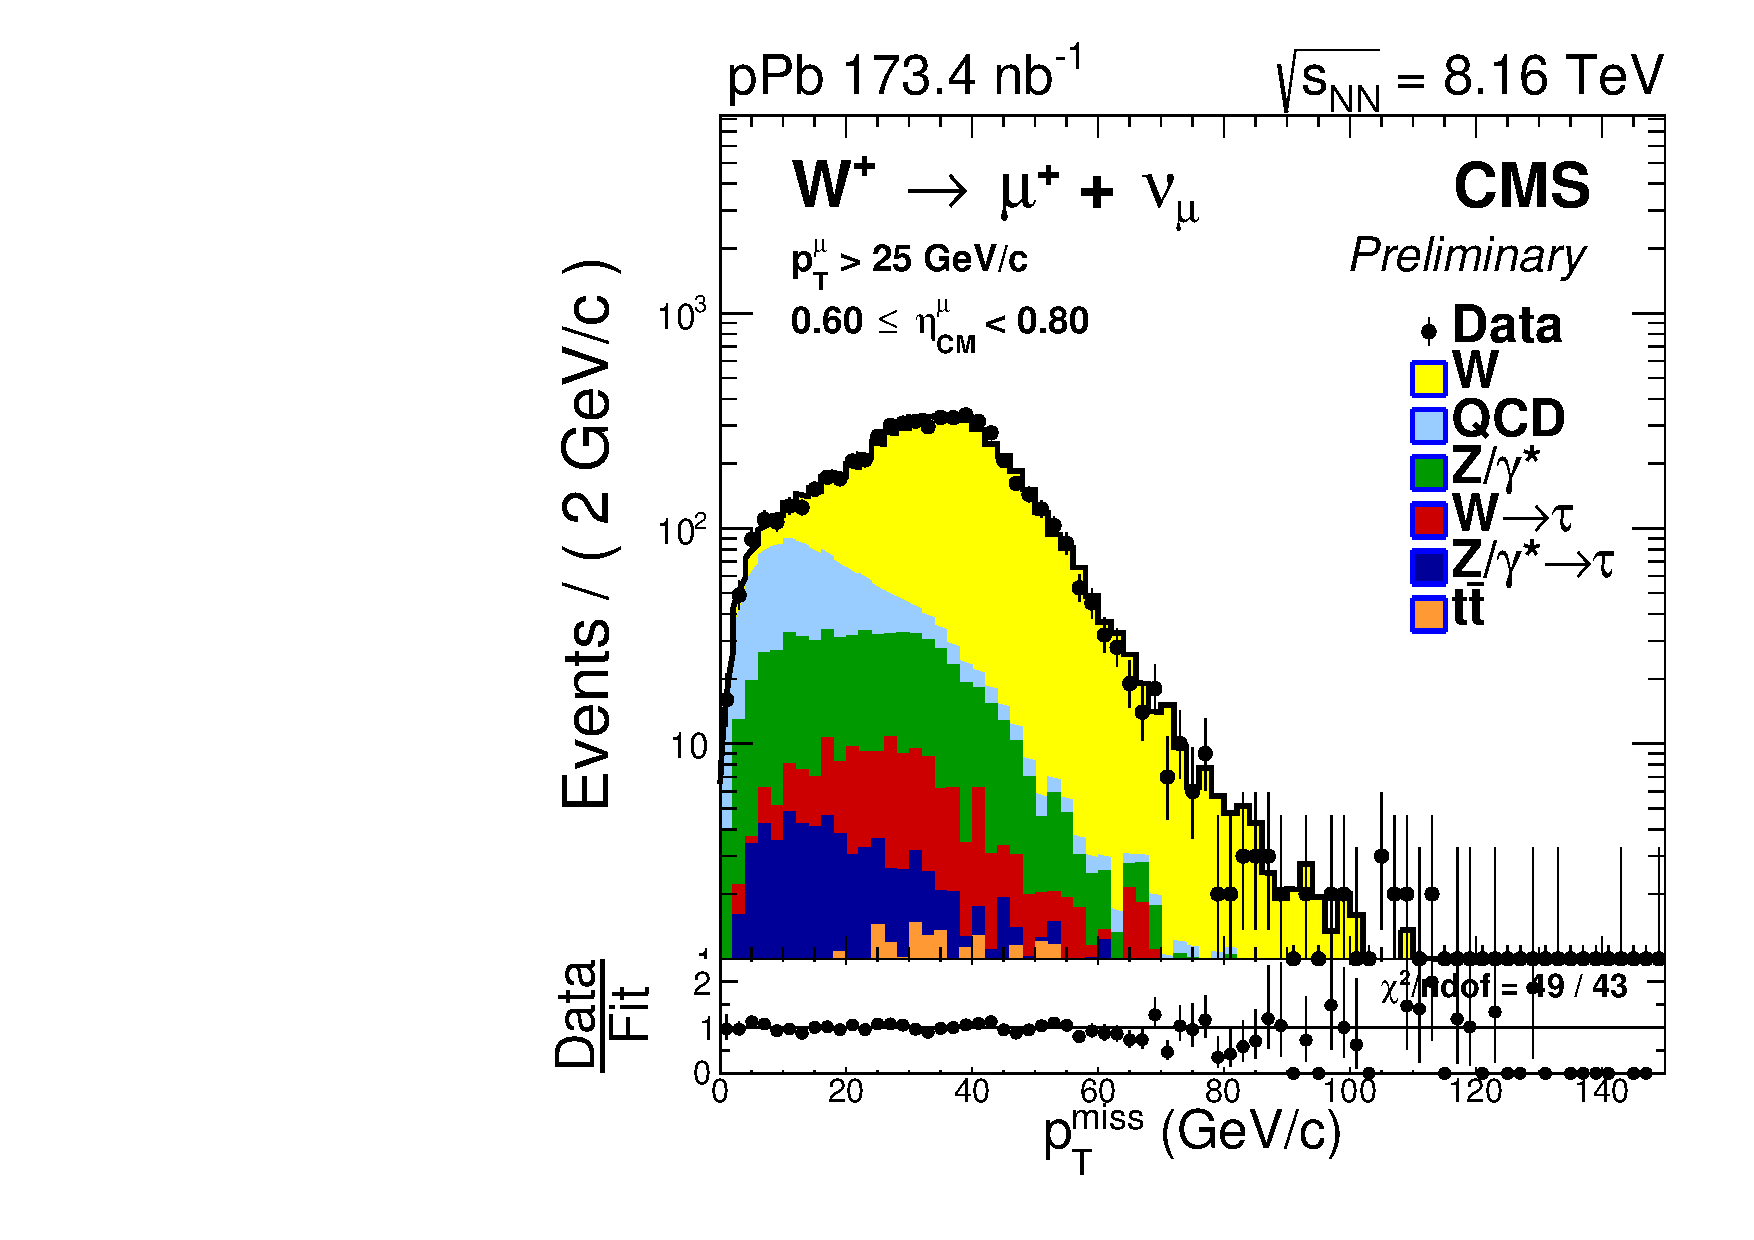
\includegraphics[width=0.23\textwidth]{Figures/WBoson/Analysis/SignalExtraction/Signal/LOG/PLOT_MET_DATA_WToMuPl_PA_Model_TEMP_WDYDYToTauWToTauTTbar_ModifiedRayleigh_QCD_MuEtaCM_60_80_MuIso_0_15.pdf}
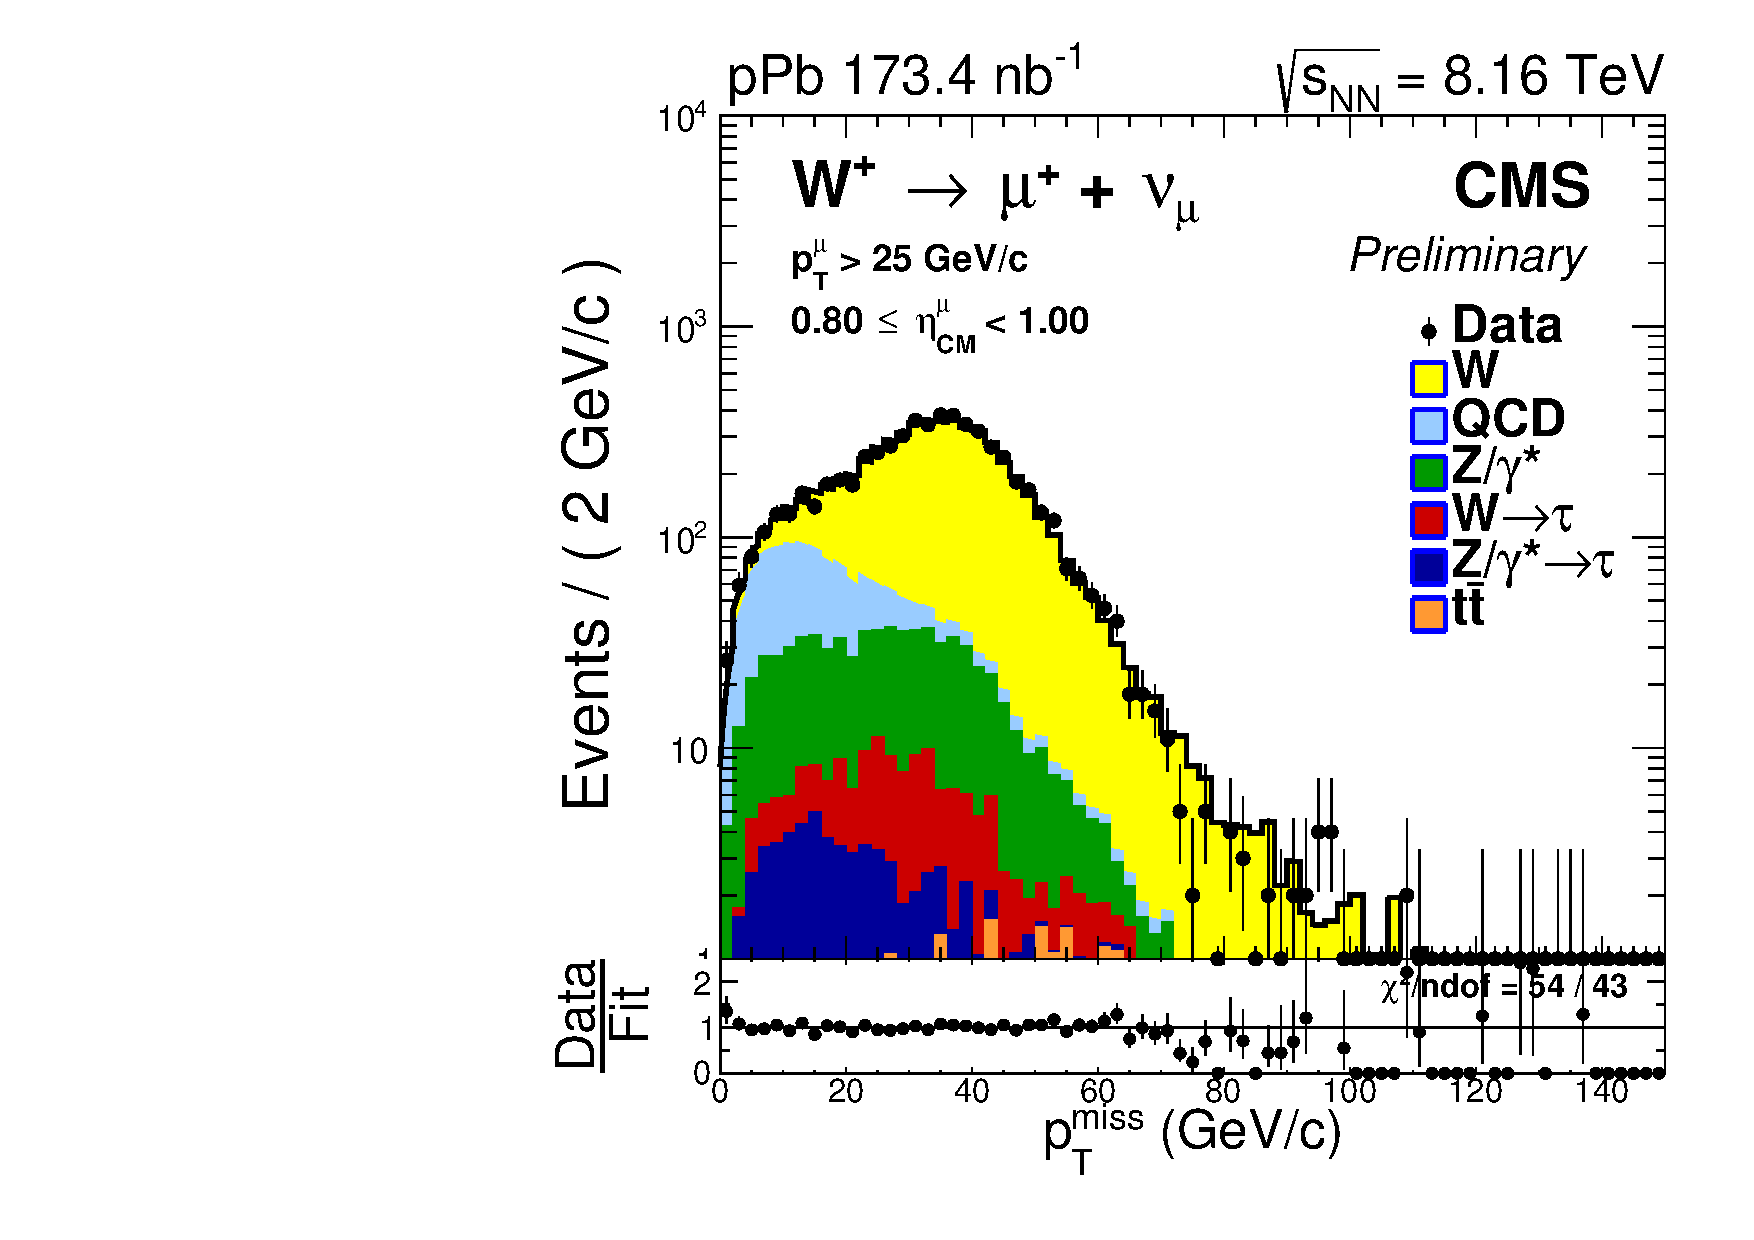
\includegraphics[width=0.23\textwidth]{Figures/WBoson/Analysis/SignalExtraction/Signal/LOG/PLOT_MET_DATA_WToMuPl_PA_Model_TEMP_WDYDYToTauWToTauTTbar_ModifiedRayleigh_QCD_MuEtaCM_80_100_MuIso_0_15.pdf}
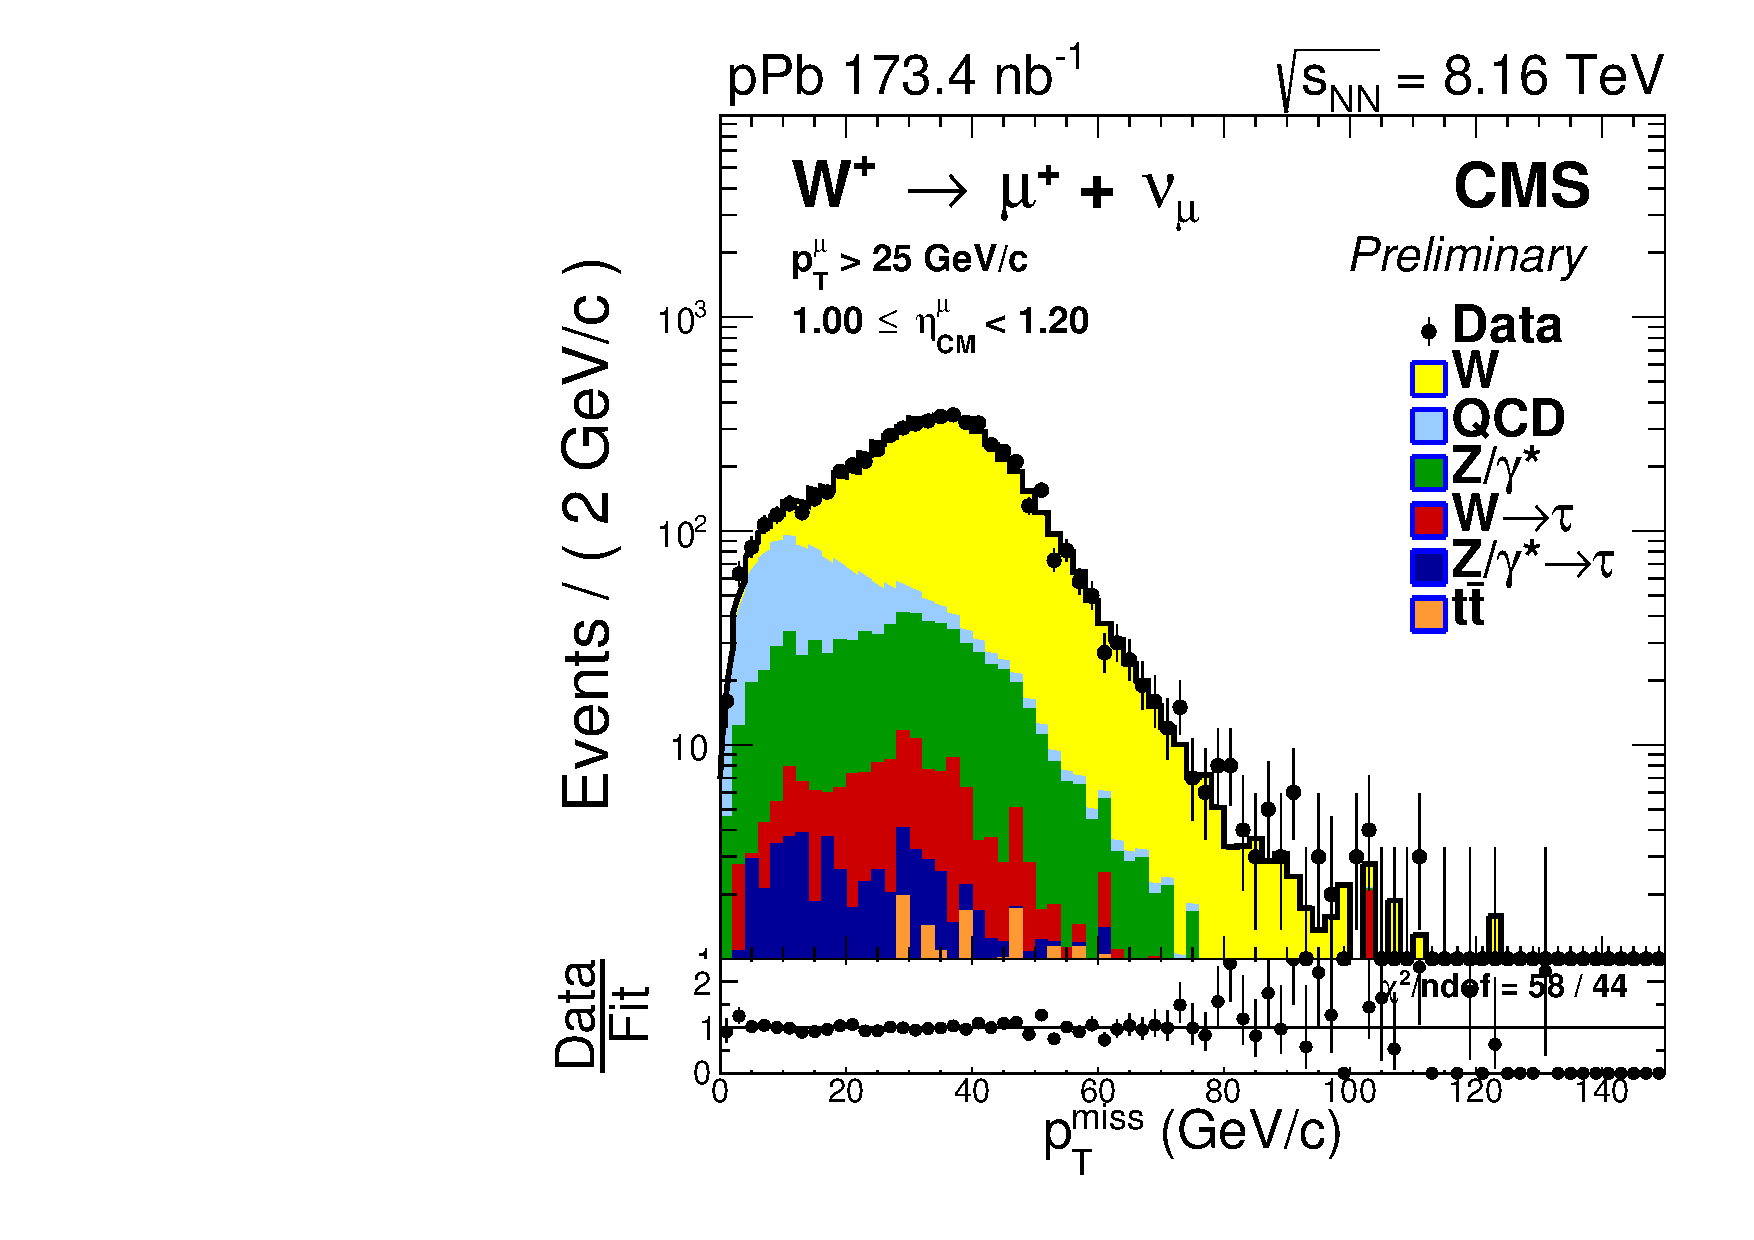
\includegraphics[width=0.23\textwidth]{Figures/WBoson/Analysis/SignalExtraction/Signal/LOG/PLOT_MET_DATA_WToMuPl_PA_Model_TEMP_WDYDYToTauWToTauTTbar_ModifiedRayleigh_QCD_MuEtaCM_100_120_MuIso_0_15.pdf}
\\
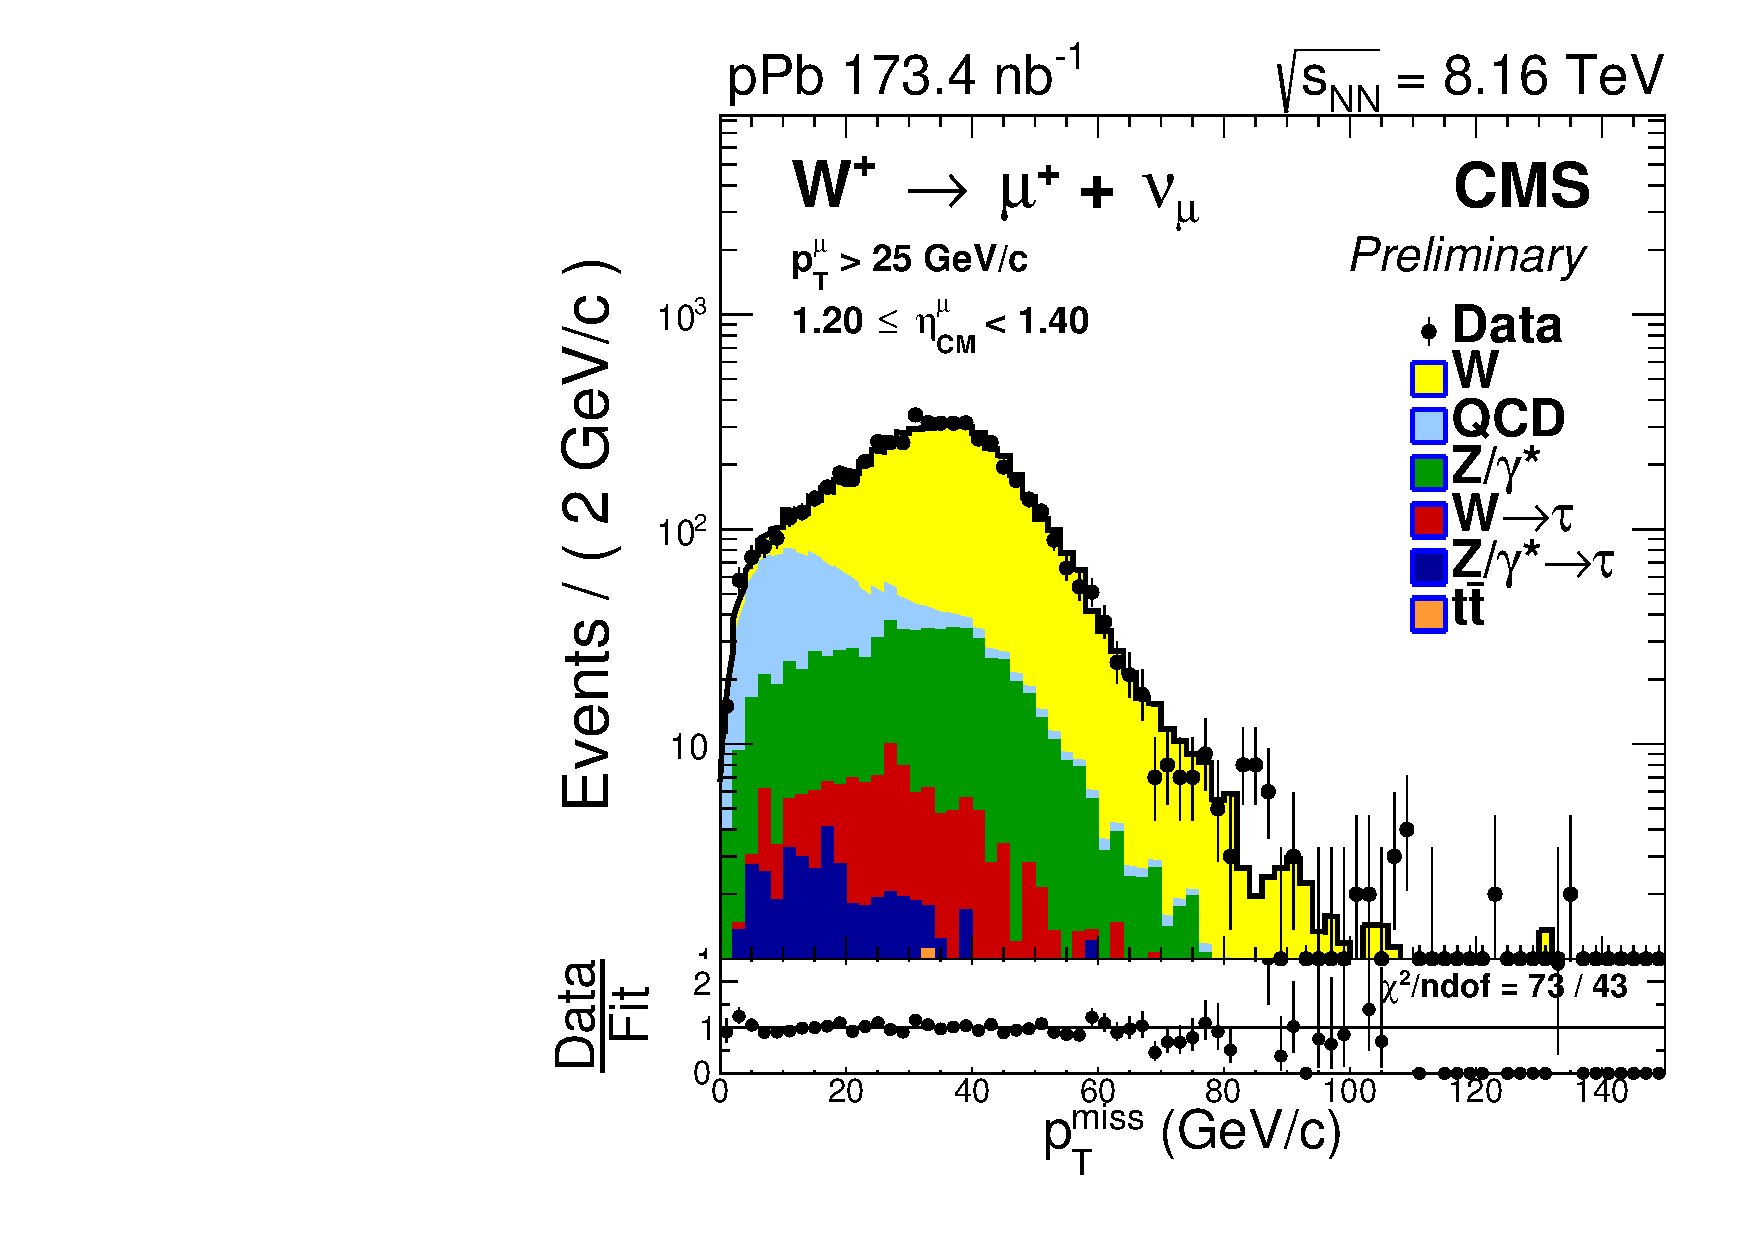
\includegraphics[width=0.23\textwidth]{Figures/WBoson/Analysis/SignalExtraction/Signal/LOG/PLOT_MET_DATA_WToMuPl_PA_Model_TEMP_WDYDYToTauWToTauTTbar_ModifiedRayleigh_QCD_MuEtaCM_120_140_MuIso_0_15.pdf}
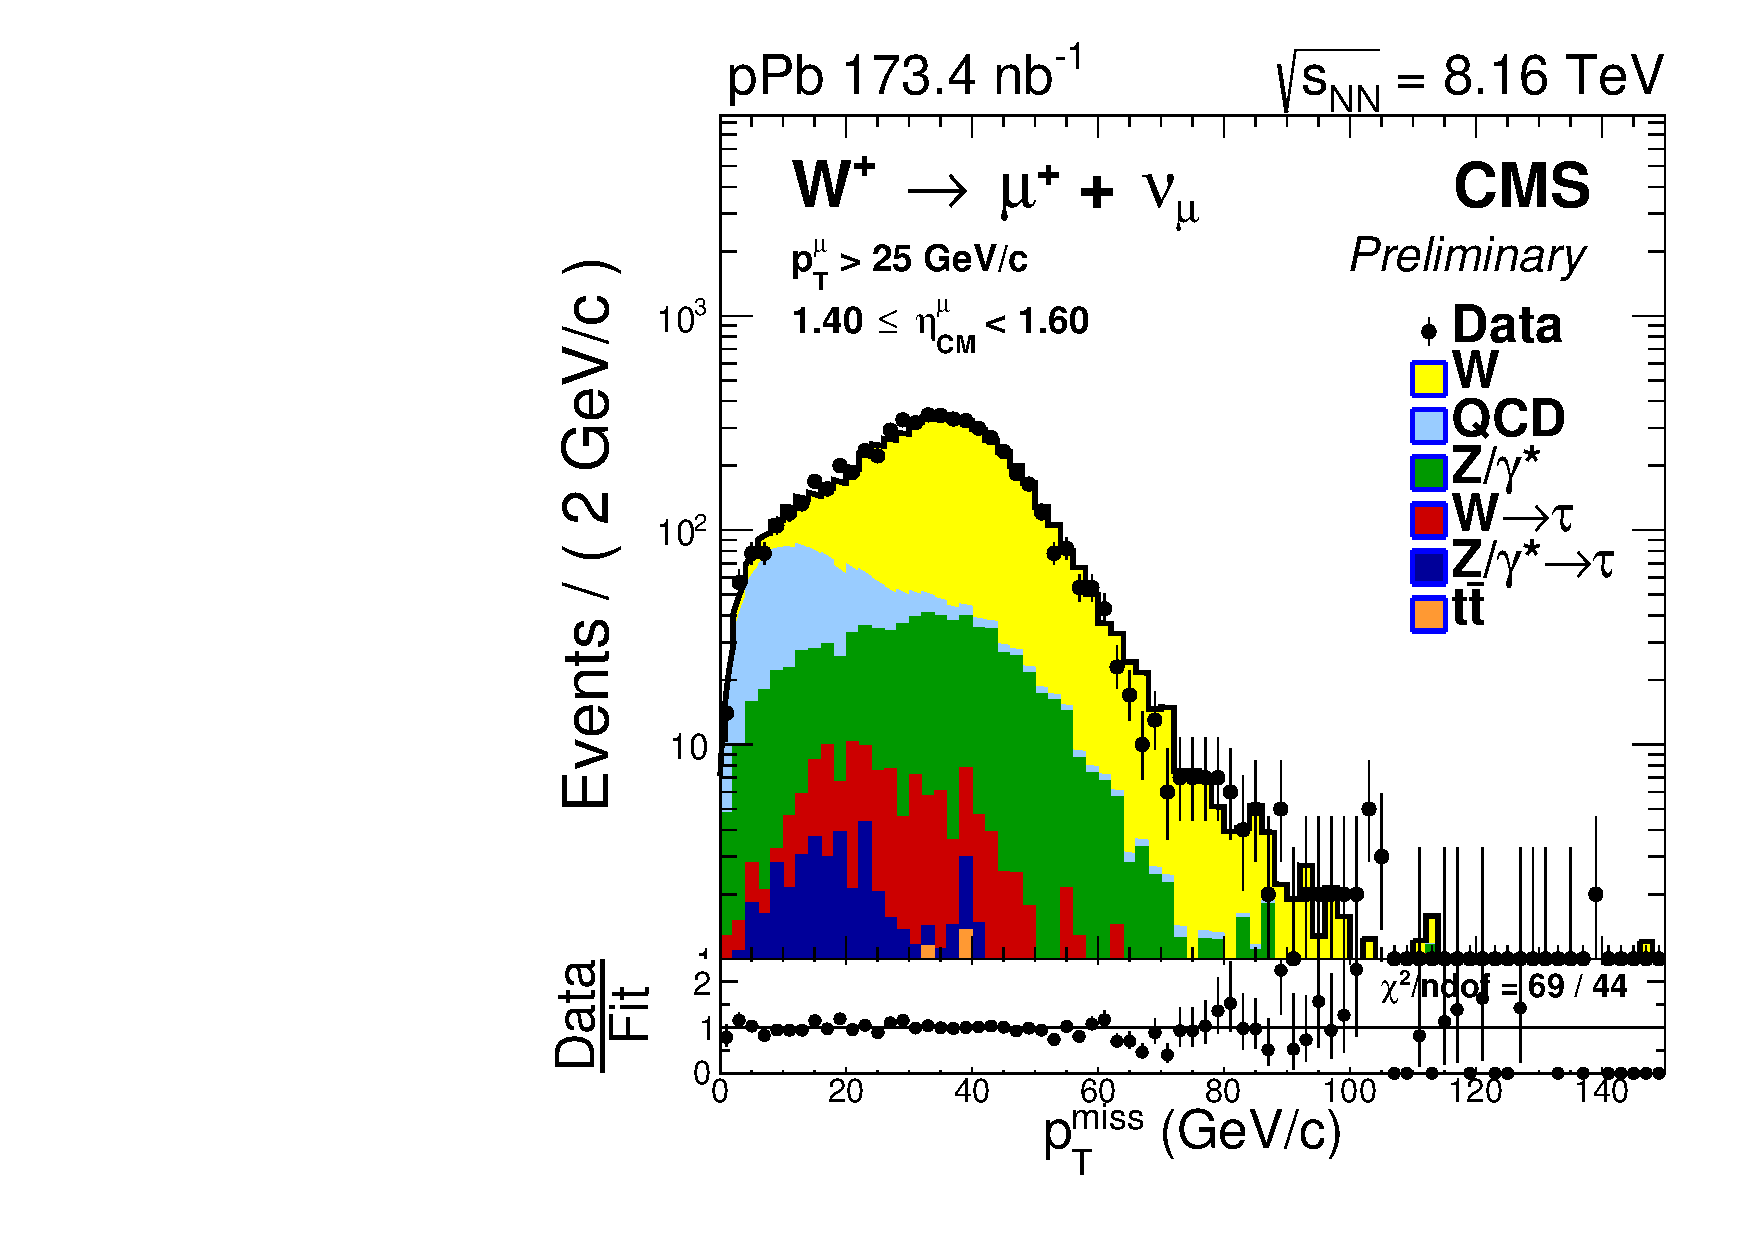
\includegraphics[width=0.23\textwidth]{Figures/WBoson/Analysis/SignalExtraction/Signal/LOG/PLOT_MET_DATA_WToMuPl_PA_Model_TEMP_WDYDYToTauWToTauTTbar_ModifiedRayleigh_QCD_MuEtaCM_140_160_MuIso_0_15.pdf}
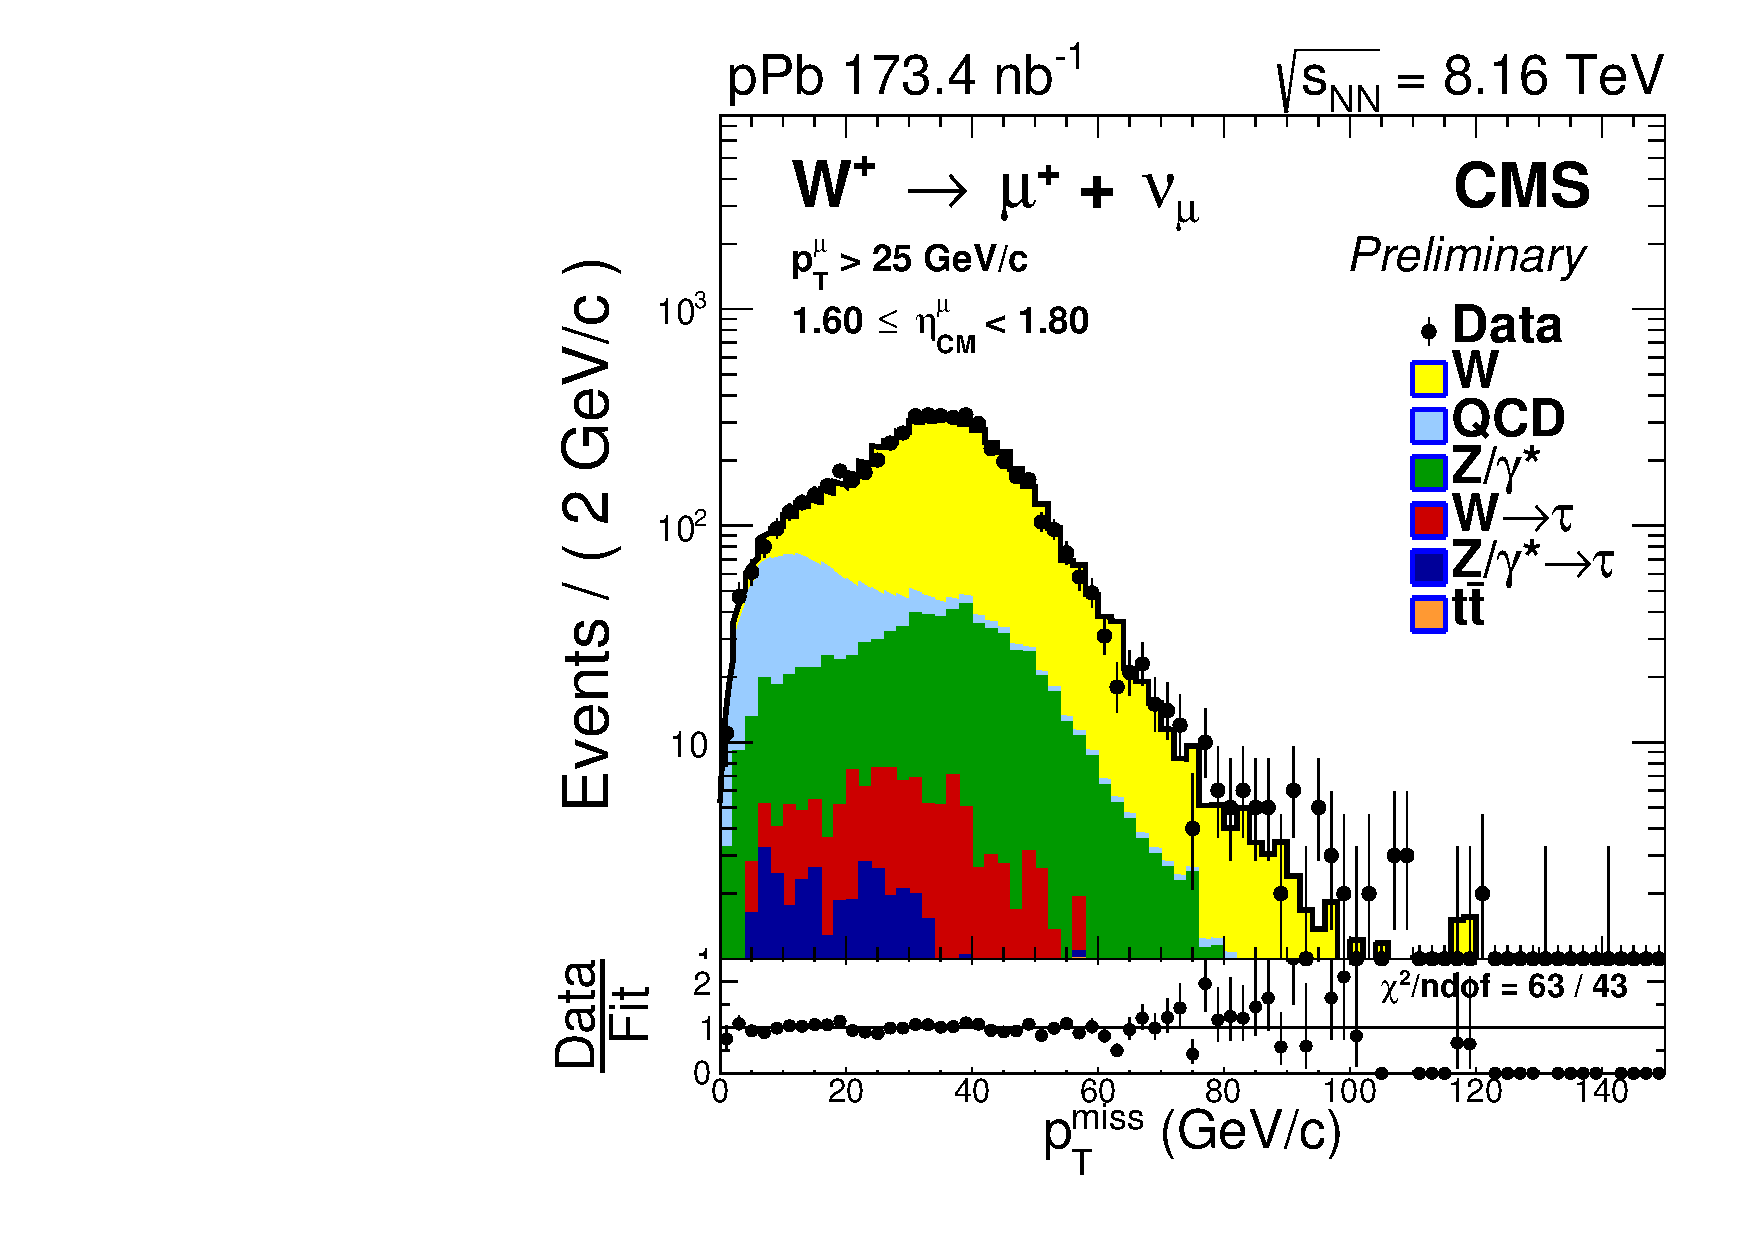
\includegraphics[width=0.23\textwidth]{Figures/WBoson/Analysis/SignalExtraction/Signal/LOG/PLOT_MET_DATA_WToMuPl_PA_Model_TEMP_WDYDYToTauWToTauTTbar_ModifiedRayleigh_QCD_MuEtaCM_160_180_MuIso_0_15.pdf}
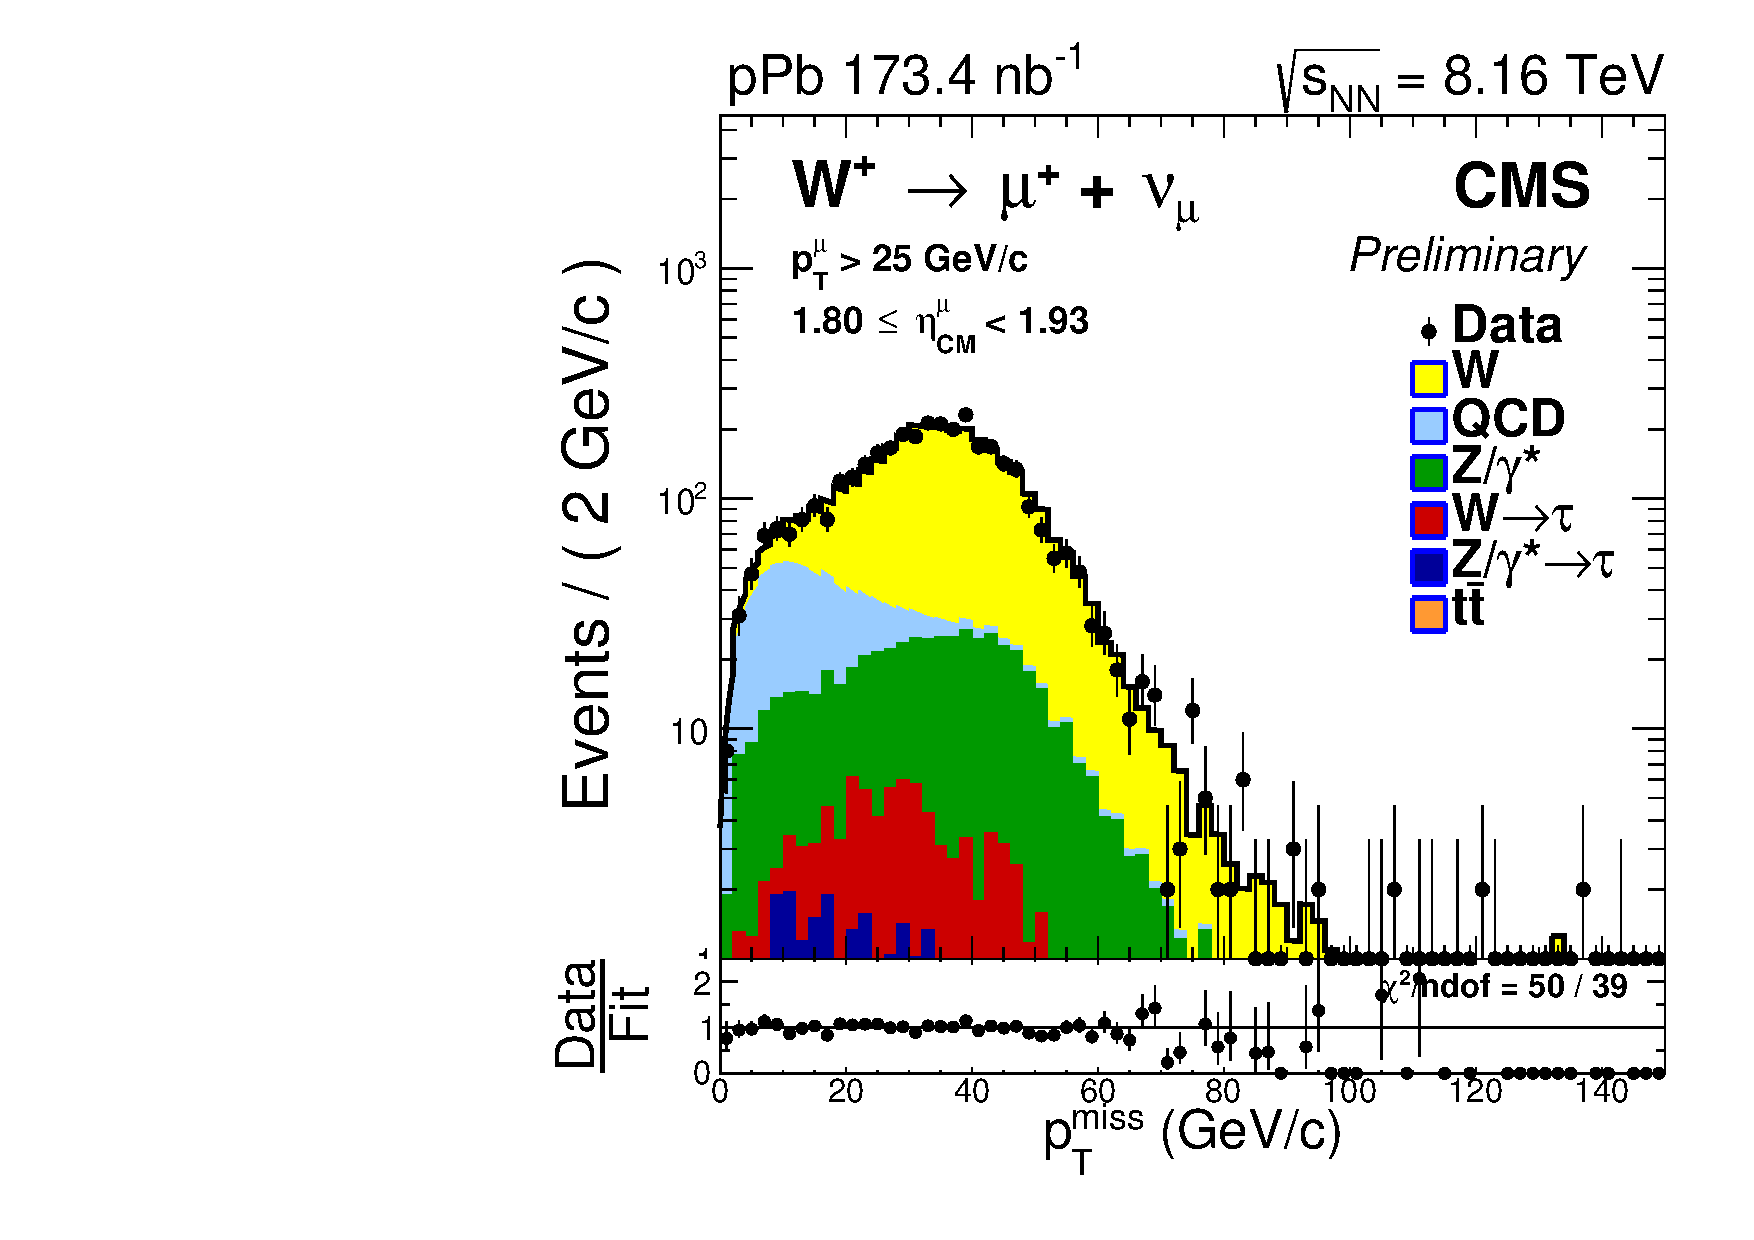
\includegraphics[width=0.23\textwidth]{Figures/WBoson/Analysis/SignalExtraction/Signal/LOG/PLOT_MET_DATA_WToMuPl_PA_Model_TEMP_WDYDYToTauWToTauTTbar_ModifiedRayleigh_QCD_MuEtaCM_180_193_MuIso_0_15.pdf}
\end{tiny}
\caption{The \ptmiss distribution for \WToMuNuPl events within each fitted \etaMuCM range, shown in logarithmic scale. Unbinned fits to the data (black points) are performed with six contributions, stacked from top to bottom: \WToMuNuPl (yellow), QCD multijet (light blue), \DYToMuMu (green), \WToTauNuPl (red), \DYToTauTau (dark blue) and \ttbar (orange). Error bars represent statistical uncertainties. The lower panels display the data divided by the result of the fit, for each \etaMuCM range. The $\chi^{2}$ test value over the number of degrees of freedom is also shown.}
\label{fig:METFits_WToMuPl_PA}
 
\end{figure}


\begin{figure}[htb!]
\centering
\begin{tiny}
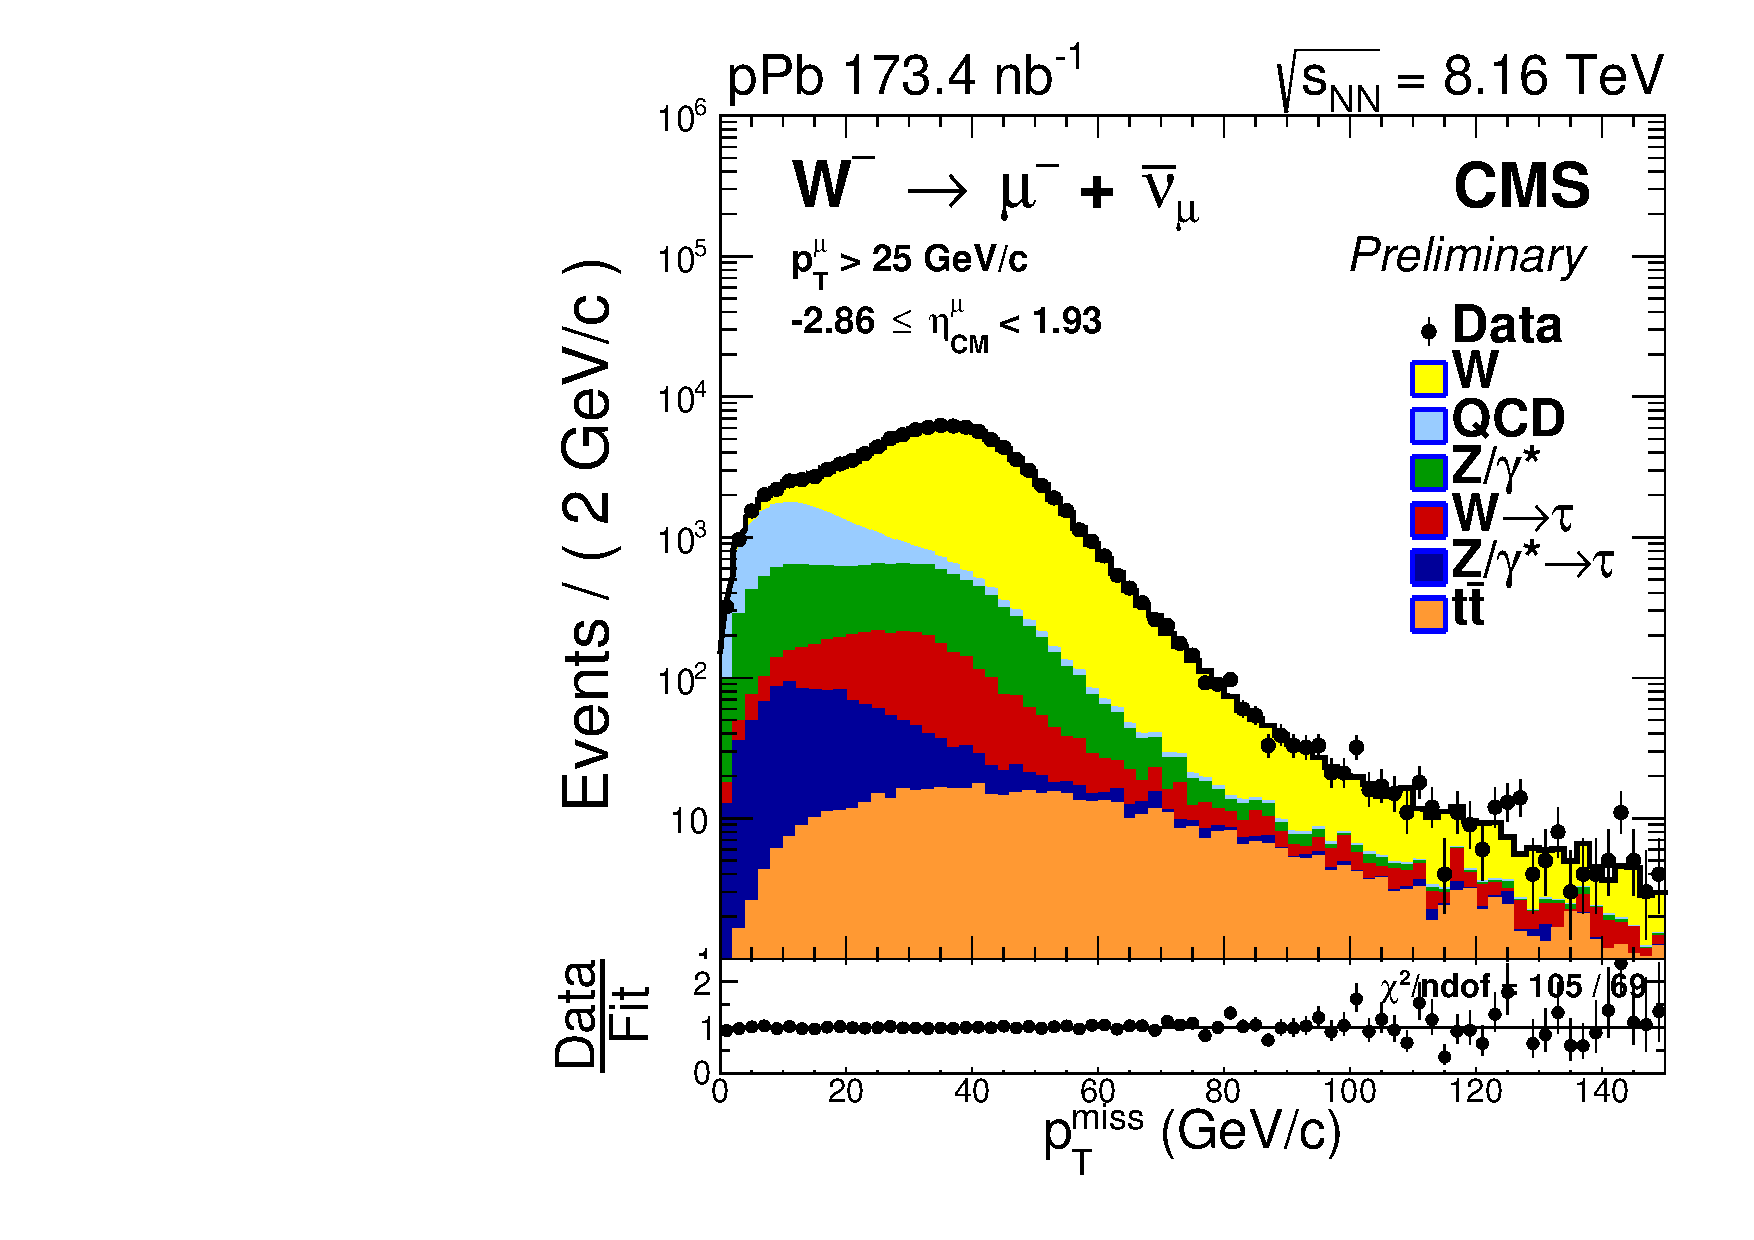
\includegraphics[width=0.45\textwidth]{Figures/WBoson/Analysis/SignalExtraction/Signal/LOG/PLOT_MET_DATA_WToMuMi_PA_Model_TEMP_WDYDYToTauWToTauTTbar_ModifiedRayleigh_QCD_MuEtaCM_-286_193_MuIso_0_15.pdf}
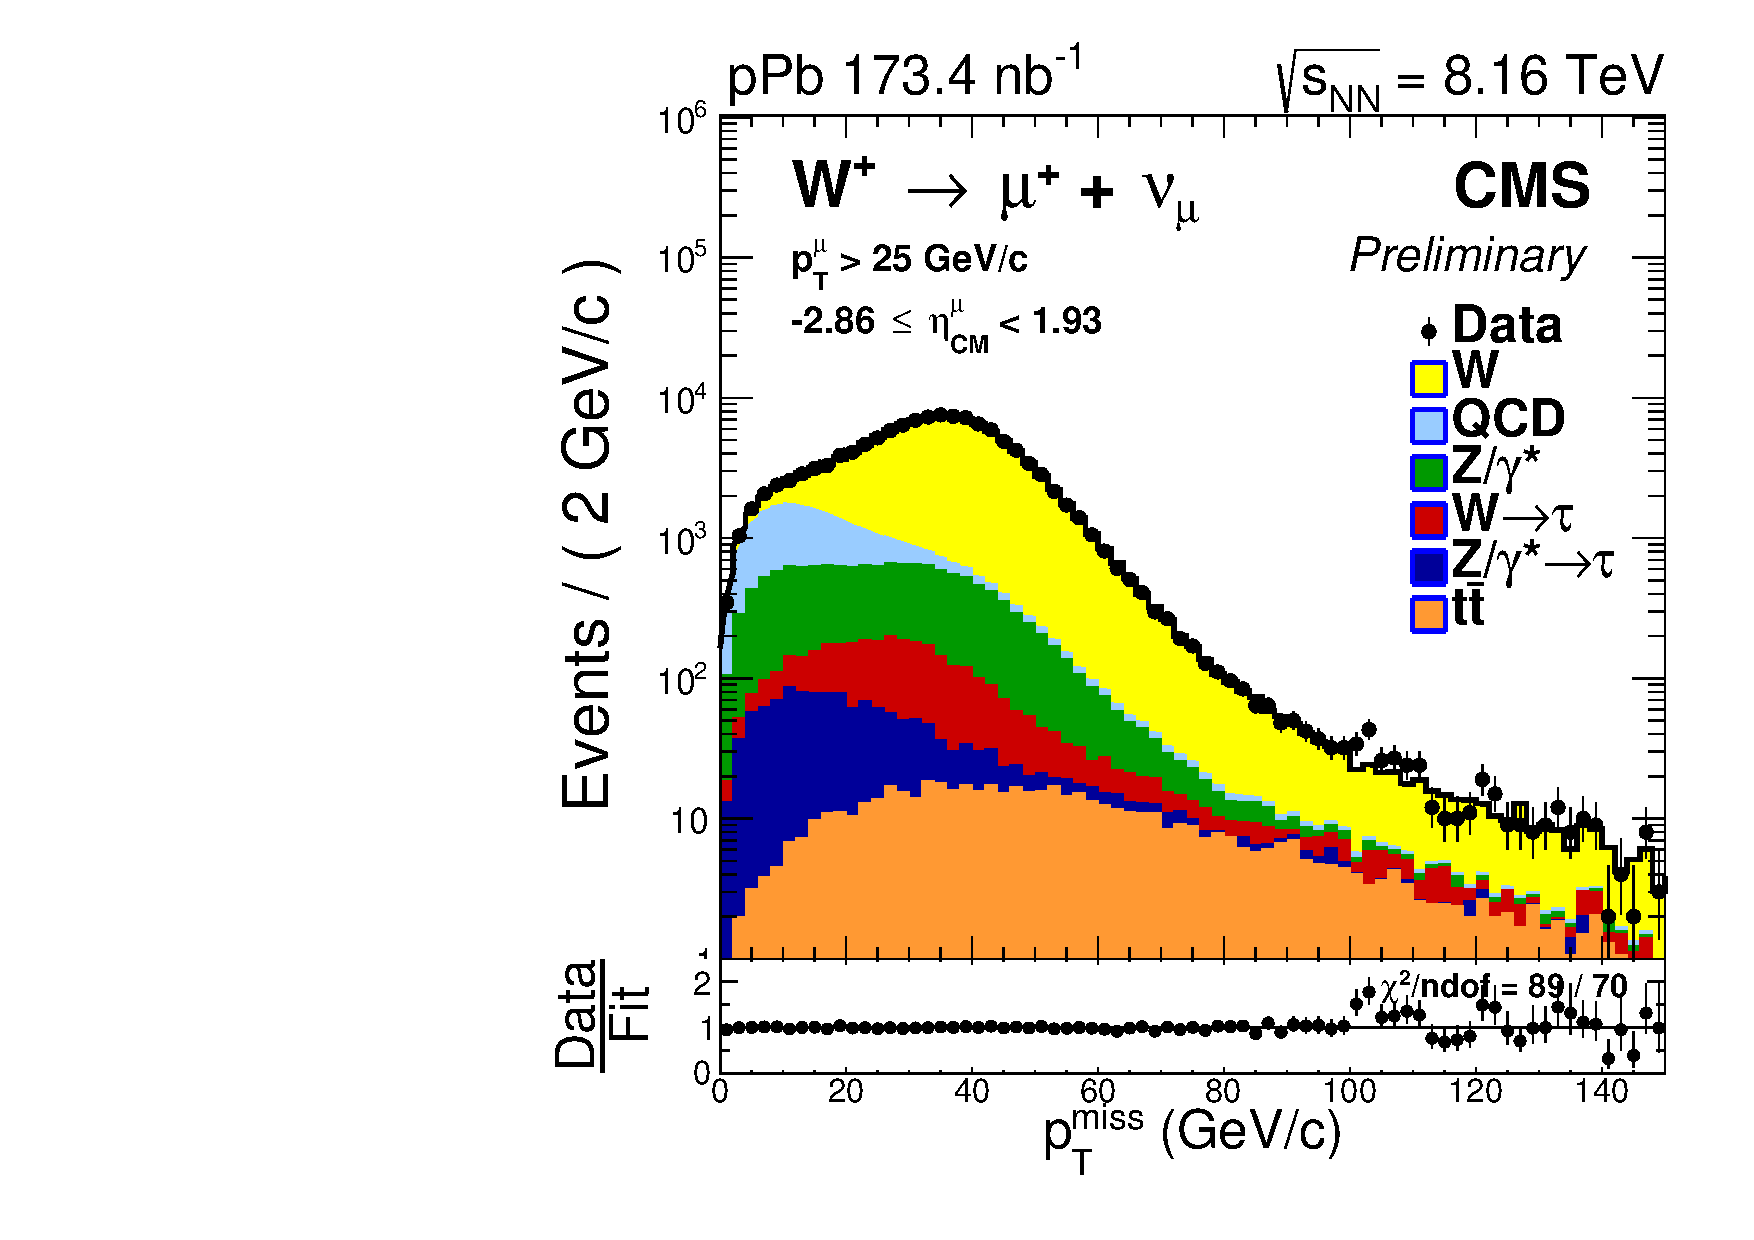
\includegraphics[width=0.45\textwidth]{Figures/WBoson/Analysis/SignalExtraction/Signal/LOG/PLOT_MET_DATA_WToMuPl_PA_Model_TEMP_WDYDYToTauWToTauTTbar_ModifiedRayleigh_QCD_MuEtaCM_-286_193_MuIso_0_15.pdf}
\end{tiny}
\caption{The \ptmiss distribution for \WToMuNuPl (left) and \WToMuNuMi (right) events within the \etaMuCM-inclusive range, shown in logarithmic scale. Unbinned fits to the data (black points) are performed with six contributions, stacked from top to bottom: \WToMuNu (yellow), QCD multijet (light blue), \DYToMuMu (green), \WToTauNu (red), \DYToTauTau (dark blue) and \ttbar (orange). Error bars represent statistical uncertainties. The lower panels display the data divided by the result of the fit, for each \etaMuCM range. The $\chi^{2}$ test value over the number of degrees of freedom is also shown.}
\label{fig:METFits_WToMuPl_PA_Inc}
 
\end{figure}
